% DER_XIIc-a: Grothendieck's text with the commentary set in, then the overview, inside a group that applies the chunk's own definitions
\dgrpart{1}{XIIc-a}{Section 6, part 1 of 2, manuscript pages 171--234}{XIIc-a\enspace\textperiodcentered\enspace Chapter XII, section 6, part 1 of 2\enspace\textperiodcentered\enspace manuscript pages 171--234}{Chapter XII \textperiodcentered\ \textup{XIIc-a}}
\dgrchunkbegin
% DER_XIIc-a: the definitions of the chunk's preamble, applied inside its group
\let\printedpage\relax\newcommand{\printedpage}[1]{{\reversemarginpar\marginnote{\raggedleft\scriptsize ed.~#1}}}
\let\msp\relax\newcommand{\msp}[1]{\marginpar{\raggedright\scriptsize ms.~#1}}
\let\Ch\relax\newcommand{\Ch}{\underline{\mathrm{Ch}}}
\let\Hotp\relax\newcommand{\Hotp}[1]{\mathrm{Hot}_{\bullet\,#1}}
\let\hotp\relax\newcommand{\hotp}[1]{\mathrm{hot}_{\bullet\,#1}}
\let\Ob\relax\newcommand{\Ob}{\mathrm{Ob}\,}
\let\HomEns\relax\newcommand{\HomEns}{\mathrm{Hom}_{\mathrm{Ens}}}
\let\utpi\relax\newcommand{\utpi}{\underset{\sim}{\pi}}
\let\Fib\relax\newcommand{\Fib}{\underline{\mathrm{Fib}}}
\let\Fl\relax\newcommand{\Fl}{\underline{\mathrm{Fl}}}
\let\Hom\relax\newcommand{\Hom}{\underline{\mathrm{Hom}}}
\let\Cat\relax\newcommand{\Cat}{\mathrm{Cat}}
\let\HOT\relax\newcommand{\HOT}{\mathrm{HOT}}
\let\Hot\relax\newcommand{\Hot}{\mathrm{Hot}}
\let\hot\relax\newcommand{\hot}{\mathrm{hot}}
\let\id\relax\newcommand{\id}{\mathrm{id}}
\let\cM\relax\newcommand{\cM}{\mathcal{M}}
\let\cF\relax\newcommand{\cF}{\mathcal{F}}
\let\Ho\relax\newcommand{\Ho}{\mathrm{Ho}}
\let\ho\relax\newcommand{\ho}{\mathrm{ho}}
\let\Wu\relax\newcommand{\Wu}{W^{\mathrm{u}}}
\let\lc\relax\newcommand{\lc}{\mathrm{lc}}
\let\circled\relax\newcommand{\circled}[1]{\tikz[baseline=(c.base)]\node[draw,circle,inner sep=1pt](c){#1};}
\let\deff\relax\newcommand{\deff}{\overset{\text{déf}}{=}}

\selectlanguage{french}


% ---- from Der-ChXIIc-30-03-03_p001-005.tex
\printedpage{115}
% head: A. Grothendieck : Dérivateurs, Ch. XII, Édition des Universités de Montpellier II et Paris VII
% foot: Version 30 mars 2003

\msp{page 171}

\section*{VI\quad Critère de $W_\infty$-asphéricité pour les $\Omega^n(X,x)$.}

\subsection*{1\quad Cogitations sur $W_n$.}

On va définir, pour $n \in \mathbf{N}$,
\[
W_n \subseteq \mathrm{Fl}(\mathrm{Cat})
\]
par les conditions suivantes (où $f : X \longrightarrow Y$ est une flèche dans Cat).

\noindent\begin{tabular}{@{}l c l >{\RaggedRight\arraybackslash}p{0.64\textwidth}@{}}
$f \in W_0$ & $\Longleftrightarrow$ & a) & $\pi_0(f)$ bijectif.\\
 & $\Longleftrightarrow$ & b) & Pour tout préfaisceau d'ensembles $F$ \textit{constant} sur $Y$, $H^0(Y,F) \longrightarrow H^0(X,f^*F)$ est bijectif.\\
 & $\Longleftrightarrow$ & c) & Le foncteur $F \longmapsto f^*F$ des préfaisceaux d'ensembles \textit{constants} sur $Y$ vers les faisceaux d'ensembles constants sur $X$ est pleinement fidèle.
\end{tabular}

\texttt{[Les termes de faisceau ou de préfaisceau sont utilisés ici indifféremment.]}

\textbf{NB} Si $F_0$ est un ensemble, $F_{0\,Y}$ le faisceau d'ensembles constant défini par $F$ sur $Y$, on a
\[
\begin{aligned}
H^0(Y,F_{0\,Y}) &\simeq \HomEns(\pi_0(Y),F_0) && \text{(fonctoriel en $Y$)}\\
\mathrm{Hom}_{Y^\wedge}(F_{0\,Y},G_{0\,Y}) &\simeq \HomEns(\pi_0(Y),\HomEns(F_0,G_0)) && \text{(fonctoriel en $Y$),}
\end{aligned}
\]
ce qui implique que a) $\Longrightarrow$ c) $\underset{\substack{\text{en prenant}\\ \mathrm{Hom}_{Y^\wedge}(e_Y,F)}}{\overset{\text{tautologiquement}}{\Longrightarrow}}$ b) $\Longrightarrow$ a).

\noindent\begin{tabular}{@{}l c l >{\RaggedRight\arraybackslash}p{0.64\textwidth}@{}}
$f \in W_1$ & $\Longleftrightarrow$ & a) & $\pi_0(f)$ bijectif, et pour tout $x \in \Ob X$, $\pi_1(f,x) : \pi_1(X,x) \longrightarrow \pi_1(Y,f(x))$ est bijectif. (NB Il suffit de le vérifier pour \textit{un} $x$ dans chaque composante connexe de $X$.)\\
 & $\Longleftrightarrow$ & a$'$) & $\Pi(X) \xrightarrow{\Pi f} \Pi(Y)$ est une équivalence de catégories.\\
 & $\Longleftrightarrow$ & b) & $H^0(Y,F) \longrightarrow H^0(X,f^*F)$ bijectif pour tout faisceau d'ensembles \textit{localement constant} sur $Y$, et $H^1(Y,F) \longrightarrow H^1(X,f^*F)$ bijectif si de plus $F$ est un faisceau en groupes.\\
 & $\Longleftrightarrow$ & b$'$) & Comme b), mais pour le $H^1$ on se borne à $F$ \textit{constant}, et on exige $H^1(f)$ \textit{surjectif} seulement.\\
 & $\Longleftrightarrow$ & c) & Le foncteur $F \longmapsto f^*F$ de la catégorie des faisceaux d'ensembles localement constants sur $Y$ vers celle des faisceaux localement constants sur $X$ est une équivalence de catégories.
\end{tabular}

\clearpage

\printedpage{116}
% head: A. Grothendieck : Dérivateurs, Ch. XII, Édition des Universités de Montpellier II et Paris VII
% foot: Version 30 mars 2003

\msp{page 172}

\dgrblock{dgrb539}{What the first two tests measure}
\begin{dcomment}{exposition}{p171}{What the first two tests measure}
Grothendieck is trying to recognize finite homotopy information without leaving the category of small categories. The two initial cases explain why locally constant coefficients, rather than arbitrary presheaves, are the appropriate witnesses. Write $BX=|NX|$ for the classifying space of $X$. A locally constant set-valued presheaf is a functor on the fundamental groupoid $\Pi(BX)$, with the variance reversed if one retains the presheaf convention. In this block all changes of variance are absorbed by inversion in the groupoid. The word ``constant'' on p.~171 means globally constant, whereas ``locally constant'' permits monodromy. For a disconnected category these are substantially different conditions.

For a set $A$, a section of the constant presheaf $A_X$ chooses one element of $A$ on each connected component. Thus $H^0(X,A_X)=\operatorname{Map}(\pi_0X,A)$. A natural transformation $A_X\to B_X$ similarly chooses one map $A\to B$ per component. These formulas prove all three tests for $W_0$. In the converse direction, if precomposition with $\pi_0f$ is bijective for every target set, Yoneda gives that $\pi_0f$ is a bijection. The empty category is included: the map from a two-element set to its set of sections on the empty category cannot be bijective.

There is a useful elementary explanation of the apparently weak condition b$'$) for $W_1$. After using constant sets to identify components, work with connected $X,Y$ and put $\alpha:H=\pi_1(X,x)\to G=\pi_1(Y,f(x))$. Sections of the local system corresponding to a $G$-set $A$ are $A^G$, and sections after pullback are $A^H$. Their equality for every $A$ forces $\alpha$ to be surjective. Indeed, let $K=\alpha(H)$ and take the transitive $G$-set $G/K$. The coset $K$ is fixed by $H$; if every $H$-fixed element is $G$-fixed, then $K=G$. Constant nonabelian $H^1$ has the familiar description
\[
 H^1(X,L_X)=\operatorname{Hom}(H,L)/L,
\]
where $L$ acts by conjugation. Surjectivity for $L=H$ says that the class of the identity of $H$ is represented by $\rho\alpha$ for some $\rho:G\to H$. Conjugating $\rho$ makes $\rho\alpha=1_H$, so $\alpha$ is injective as well. If there are several components, choose the identity representation on the chosen component and trivial representations on the others. This proves b$'$)$\Rightarrow$a), including the componentwise assertion.

An equivalence of fundamental groupoids conversely identifies every category of local systems, its global sections, and its torsors. This proves a)$\Rightarrow$b), c). To see directly that c) also forces the groupoid equivalence, full faithfulness recovers global sections as maps from the terminal object and hence forces $\alpha$ to be surjective by the same coset argument; essential surjectivity makes the regular $H$-set the restriction of a $G$-set, so $\ker\alpha$ acts trivially on a faithful $H$-set and is trivial. The torsor interpretation is the first step of the comparison between cohomology and homotopy types recalled in \citet[Preface, pp.~vii--viii]{Lurie2009HTT}. Nothing here requires a choice of a universal covering category: the fundamental groupoid already contains precisely the needed information.
\end{dcomment}


\textbf{NB} Le groupe $\pi_1(X,x)$ est défini via la théorie du groupoïde fondamental. On sait qu'il est en bijection canonique avec $\pi_0(\Omega(X,x))$, où $\Omega(X,x) = \Ch(X;x,x)$ (ce qui permet d'avoir une loi de composition monoïdale sur $\Omega(X,x)$, donnant la loi de groupe sur le $\pi_0$), ou au choix $\Omega(X,x) = \Ch_\infty(X;x,x)$ (plus commode dans certaines situations, mais ne donnant pas directement la loi de composition dans $\pi_0(\Omega(X,x))$).

Je vais poser, pour $n \in \mathbf{N}$,
\[
\pi_n(X,x) = \pi_0(\Omega^n(X,x)),
\]
$\Omega^n$ désignant l'itéré $n$-ième du foncteur $(X,x) \longmapsto \Omega(X,x)$ de la catégorie $\mathrm{Cat}_\bullet$ des objets ponctués de Cat dans elle-même. Je préfère ici travailler avec la théorie \underline{Ch} au lieu de $\Ch_\infty$. Tôt ou tard il faudra donner un énoncé de comparaison \dots

\textbf{Théorème 1} (\footnote[112]{Sans doute \textit{faux}. On doit avoir a) $\Longrightarrow$ b), mais b) $\Longrightarrow$ a) \texttt{[est]} sans doute faux déjà pour $n = 2$ (sauf le cas $X$, $Y$ 1-connexes). Cf. énoncé rectifié \texttt{[p. 178]}.}). \textit{Soit $f : X \longrightarrow Y$ dans} Cat\textit{, et soit $n \in \mathbf{N}$, $n \geq 2$, $S$ une partie de} $\Ob X$ \textit{telle que le composé $S \longrightarrow \Ob X \longrightarrow \pi_0(X)$ soit} \texttt{[un]} \textit{épimorphisme. Les conditions suivantes sont équivalentes.}

\begin{itemize}
\item[\textit{a)}] \textit{$\pi_i(f,x)$ isomorphe pour tout $x \in \Ob X$ et tout $i \in [0,n]$.}

\item[\textit{a$'$)}] \textit{Comme a), mais avec $x \in S$.}

\item[\textit{b)}] \textit{On a}
\[
\begin{array}{rcll}
H^0(Y,F) & \xrightarrow{\ \sim\ } & H^0(X,f^*F) & \textit{pour $F$ faisceau d'ensembles}\\
 & & & \textit{localement constant sur $Y$.}\\
H^1(Y,F) & \xrightarrow{\ \sim\ } & H^1(X,f^*F) & \textit{si de plus $F$ faisceau en groupes.}\\
H^i(Y,F) & \xrightarrow{\ \sim\ } & H^i(X,f^*F) & \textit{si de plus $F$ faisceau abélien, $i \in [2,n]$.}
\end{array}
\]
\end{itemize}

\msp{page 173}

\dgrblock{dgrb540}{Loops, finite types, and the scope of the proposed theorem}
\begin{dcomment}{exposition}{p172}{Loops, finite types, and the scope of the proposed theorem}
The iterated path construction is being asked to do two jobs. First it supplies the groups $\pi_i(X,x)$ intrinsically in $\Cat$; subsequently it must show that these groups are the usual homotopy invariants of $BX$. The later identification of the minimal fundamental localizer with ordinary weak homotopy equivalences removes the distinction between $W_\omega$ and $W_\infty$ in the modern interpretation; see \citet[Theorem~2.2.11]{Cisinski2004Minimal}. It should not be used to erase Grothendieck's effort to obtain the result from the categorical path construction itself.

Theorem~1 contains three separate assertions. The equivalence a)$\Leftrightarrow$a$'$) is the basepoint transport statement established below. The implication a)$\Rightarrow$b) is correct, and the argument on pp.~180--185 supplies its proof after the twisted-coefficient evaluation map is made explicit. The converse b)$\Rightarrow$a) is false in general. The first failure, however, is in degree $3$, not in degree $2$ as footnote~112 suggests. The degree-two case survives even with nontrivial fundamental group. We prove this distinction below, because it materially changes the interpretation of the ensuing ``rectification''.

It is also necessary to distinguish an equivalence of $n$-types from a map with $n$-connected homotopy fibres. For the former, $\pi_0f$ is bijective and $\pi_if$ is an isomorphism for $1\leq i\leq n$. For the latter one needs, in addition, surjectivity on $\pi_{n+1}$. Grothendieck identifies this additional condition correctly on p.~179, but calls the fibre condition the ``good localizer'' on p.~187. That last sentence cannot stand as a definition of a class of weak equivalences: the fibre condition fails the two-out-of-three axiom. The distinction does disappear for a map to a point, which explains why the argument of Theorem~2 is unaffected.
\end{dcomment}


\textbf{NB} L'équivalence de a) et a$'$) devrait être triviale, mais pour cela il faut avoir défini les $\pi_n(X,x)$, pour $x$ variable dans $\Ob X$, comme système local sur $X$, chose que je n'ai pas faite encore. Je vais essayer de le faire dans un courant d'air. Tout d'abord, les $\Omega(X,x)$ sont les fibres d'une $W_\omega$-fibration parfaite (\footnote[113]{\textbf{NB} $W_\omega$ est le plus petit localiseur de Cat (satisfaisant W(1, 2 bis, 3)).}), s'insérant dans le carré cartésien
\[
\begin{tikzcd}
\Ch(X) \arrow[d, "{p_X=(\sigma_X,\beta_X)}"'] & \Omega(X,-) \arrow[l] \arrow[d] \\
X \times X & X. \arrow[l, "\mathrm{diag}_X"'] \arrow[ul, dotted, "i_X"']
\end{tikzcd}
\]

\clearpage

\printedpage{117}
% head: A. Grothendieck : Dérivateurs, Ch. XII, Édition des Universités de Montpellier II et Paris VII
% foot: Version 30 mars 2003

On sait alors que l'on a un foncteur
\[
\begin{aligned}
\Pi X &\longrightarrow \mathrm{Hot}_{W_\omega}\\
x &\longmapsto \mathrm{hot}_{W_\omega}(\Omega(X,x)).
\end{aligned}
\tag*{$(*)$}
\]
Or on a, pour $i \geq 1$,
\[
\pi_i(X,x) = \pi_{i-1}(\ \underbrace{\Omega(X,x)}_{\text{objet ponctué}}\ ).
\]
Cela donne le système local cherché des $\pi_i$, si seulement on avait un foncteur un peu plus précis que $(*)$, savoir
\[
\Pi X \longrightarrow \Hotp{W_\omega} \qquad \text{(catégorie $W_\omega$-homotopique \textit{ponctuée})}
\]
(\footnote[114]{Mais il faut aussi vérifier que les $\pi_n(X,x)$ ($n \geq 1$) sont des foncteurs sur $\Hotp{W_\infty}$, i.e. transforment $W_\infty$-équivalences en itou. Cela résulte de W(4a) pour $W_\infty$, qui implique que $(X,x) \mapsto \Omega(X,x)$ se factorise par $\Hotp{W_\infty}$ (en tant que foncteur à valeurs dans $\Hotp{W_\infty}$).}). Or la flèche $i_X : X \longrightarrow \Ch X$ relevant $p_X$ donne une section canonique de $\Omega(X,-)$ sur $X$ -
\msp{page 174}
celle justement qui associe à tout $x \in X$ le point marqué $1_x$ de $\Omega(X;x,x)$ (`lacet vide en $x$'). La question est donc celle-ci :

\begin{quote}
On a une $W$-fibration $\Omega \longrightarrow X$, avec une section donné $\sigma$. Cela définit-il un foncteur canonique % [sic] donné -> donnée, accord avec « section »
\[
X \longrightarrow \Hotp{W},
\]
transformant toute flèche en \texttt{[un]} isomorphisme?
\end{quote}

L'idée naturelle est de prendre
\[
x \longmapsto \hotp{W}(\Omega/x)
\]
en ponctuant $\Omega/x$ par le point marqué $\sigma(x)$ de $\Omega_x \hookrightarrow \Omega/x$. L'ennui, c'est que les morphismes de transition $\Omega/x \longrightarrow \Omega/x'$ (pour $x \xrightarrow{u} x'$ dans $X$) ne sont pas compatibles avec les points marqués. Mais on a une flèche (savoir $\sigma(u)$) allant
\msp{page 175}
de l'image $\sigma(x)/x'$ du point marqué de $\Omega/x$ vers le point marqué $\sigma(x')/x'$ de $\Omega/x'$. Ceci doit suffire pour définir la flèche
\[
(\Omega/x,\sigma(x)/x) \longrightarrow (\Omega/x',\sigma(x')/x')
\]
comme flèche dans $\Hotp{W}$, avec transitivité pour une composée $x \xrightarrow{u} x' \xrightarrow{v} x''$ dans $X$. Je vais pour l'instant me borner
\printedpage{118}
% head: A. Grothendieck : Dérivateurs, Ch. XII, Édition des Universités de Montpellier II et Paris VII
% foot: Version 30 mars 2003
\msp{page 176}
à une indication, quitte à faire des vérifications circonstanciées par la suite. Au besoin, j'utiliserai dès maintenant que pour $i \in \mathbf{N}$, $i \geq 1$,
\[
\pi_i(f,x) : \pi_i(X,x) \longrightarrow \pi_i(Y,f(x))
\]
peuvent s'interpréter comme provenant d'un homomorphisme de systèmes locaux
\[
\utpi_i(X,-) \longrightarrow f^*(\utpi_i(Y,-))
\]
sur $X$. La condition a) du théorème 1 s'interprète en disant que cet homomorphisme est un \textit{isomorphisme} pour $i \in [1,n]$, et la condition a$'$) se borne alors à rappeler qu'il suffit de tester qu'il en est ainsi pour \textit{un} point de chaque composante connexe de $X$.

\dgrblock{dgrb541}{Making pointed transport explicit}
\begin{dcomment}{development}{p175}{Making pointed transport explicit}
Grothendieck needs to transport a marked object along an arrow even when the underlying transition functor does not preserve that object strictly. The discrepancy is useful data: the arrow supplied by the section tells us exactly which change of basepoint to make. The following construction fills in the indicated verification using only arrow categories and localization. We checked the natural-homotopy and adjunction lemmas in \citet[\S1.1, especially Proposition~1.1.9 and Corollary~1.1.10]{Cisinski2004Minimal}; we did not locate a discussion of this particular pointed comma-category formula in the consulted sources. The result is an elementary completion of the manuscript's construction, with no assertion of priority.

\textbf{Pointed transport lemma.}\ours\ Suppose $W$ contains every functor admitting a left or a right adjoint and satisfies two-out-of-three. In the localization of pointed categories at functors whose underlying functors lie in $W$, an arrow $a:d\to e$ of a category $D$ defines a canonical isomorphism
\[
 t_a:(D,d)\longrightarrow(D,e).
\]
It is natural in functors $D\to D'$, satisfies $t_{1_d}=1$, and satisfies $t_{ba}=t_bt_a$ for composable arrows $a,b$.

\textit{Proof.} Regard $a$ as the marked object of $D^{[1]}$. The two evaluation functors give a pointed span
\[
 (D,d)\xleftarrow{\ e_0\ }(D^{[1]},a)
 \xrightarrow{\ e_1\ }(D,e).
\]
The constant-diagram functor is left adjoint to $e_0$ and right adjoint to $e_1$, so both evaluations belong to $W$. Define $t_a=[e_1][e_0]^{-1}$. For the identity arrow the constant-diagram functor is a pointed common section, proving the unit assertion. For a composable pair, mark $D^{[2]}$ by the diagram $d\xrightarrow a e\xrightarrow b h$. Evaluation at every vertex belongs to $W$. For the endpoints this again follows from adjunctions. For the middle vertex use the natural transformation $e_0\Rightarrow e_1$ and the following elementary consequence of the assumptions: naturally related functors belong to $W$ simultaneously. Indeed, represent a natural transformation by $H:A\times[1]\to B$. The projection $A\times[1]\to A$ has an adjoint and lies in $W$; each endpoint section lies in $W$ by two-out-of-three. Thus $H i_0\in W$ if and only if $H\in W$, if and only if $H i_1\in W$. Restriction to the three edges commutes with vertex evaluation and is therefore in $W$ by two-out-of-three. On this common pointed source,
\[
 [e_2][e_0]^{-1}
 =\bigl([e_2][e_1]^{-1}\bigr)
  \bigl([e_1][e_0]^{-1}\bigr).
\]
This is the composition assertion. Applying a functor to arrow diagrams commutes strictly with all evaluations and restrictions, proving naturality.\hfill$\square$

Now let $q:E\to X$ be the fibration under discussion, with section $\sigma$. For $u:x\to x'$ write $u_*:E/x\to E/x'$ for postcomposition. Its marked source maps to $u_*\sigma(x)$, and the section gives an arrow
\[
 a_u:u_*\sigma(x)\longrightarrow\sigma(x')
\]
in $E/x'$. Define the pointed transition to be $t_{a_u}[u_*]$. For $v:x'\to x''$, the equality $a_{vu}=a_v\,v_*(a_u)$, naturality of $t$, and the composition formula prove the functor law. When the comma transitions belong to $W$, these maps are isomorphisms and the functor factors through $\Pi X$. The pointed inclusions $E_x\to E/x$ identify it with the family of strict fibres whenever those inclusions belong to $W$. Applied to the loop fibration, this gives the local systems of higher homotopy groups and proves the equivalence of the one-basepoint and every-basepoint formulations. It gives ordinary transport in the pointed homotopy category; a coherent family of pointed spaces contains further information, which is not claimed to follow from this ordinary functor alone.
\end{dcomment}


L'énoncé du théorème 1 garde un sens pour $n = 1$, et dans ce cas a été `rappelé' précédemment (et est $\pm$ tautologique). Cela va nous permettre de procéder par récurrence sur $n$, en supposant que le théorème est prouvé pour $n-1$. Cela signifie que l'on peut supposer que les conditions a) \textit{et} b) sont satisfaites par $f$ pour $i \in [1,n-1]$, et se borner à prouver que, sous ces conditions, la condition a) (ou a$'$), pour $i = n$, équivaut à la condition b) pour $i = n$.

\msp{page 177}

Donc il faut prouver simplement ceci :

\textbf{Lemme} (\footnote[115]{Sans doute faux.}). \textit{Supposons que $\pi_i(f,x)$} \texttt{[est un]} \textit{isomorphisme pour $i \in [0,n-1]$ et b) satisfait pour $i \in [0,n-1]$, où $n \in \mathbf{N}$, $n \geq 2$, est fixé. Alors les conditions suivantes sont équivalentes :}

\begin{itemize}
\item[\textit{a)}] $\pi_n(f,x) : \pi_n(X,x) \longrightarrow \pi_n(Y,f(x))$ \texttt{[est un]} \textit{isomorphisme pour tout $x \in \Ob X$.}

\item[\textit{b)}] $H^n(Y,F) \xrightarrow{\sim} H^n(X,f^*F)$ \texttt{[est un]} \textit{isomorphisme pour tout faisceau abélien localement constant sur $Y$.}
\end{itemize}

Notons que $f$ induit une flèche dans $\mathrm{Cat}_\bullet$,
\[
\Omega(f,x) : \Omega(X,x) \longrightarrow \Omega(Y,f(x)),
\]
d'où
\[
\begin{tikzcd}[row sep=small]
\pi_i(\Omega(X,x)) \arrow[r] \arrow[d, dash, "\wr"'] & \pi_i(\Omega(Y,f(x))) \arrow[d, dash, "\wr"'] \\
\pi_{i+1}(X,x) \arrow[r] & \pi_{i+1}(Y,f(x)),
\end{tikzcd}
\]
s'identifiant à $\pi_{i+1}(f,x)$ :
\[
\pi_i(\Omega(f,x)) \simeq \pi_{i+1}(f,x).
\]


\printedpage{119}
% head: A. Grothendieck : Dérivateurs, Ch. XII, Édition des Universités de Montpellier II et Paris VII
% foot: Version 30 mars 2003

L'hypothèse a) du lemme implique que $\pi_i(\Omega(X,x)) \xrightarrow{\sim} \pi_i(\Omega(Y,y))$ pour $i \in [0,n-1]$. Il s'agit ici des $\pi_i$ basés en les points unités. On devra sans doute prouver que, du fait qu'il s'agit d'un morphisme de monoïdes dans Cat (satisfaisant certaines conditions?) ça reste vrai pour les $\pi_i$ en \textit{tout} point $\xi$ de $\Omega(X,n)$. Par l'hypothèse de récurrence, on saura donc que $\Omega(X,x) \longrightarrow \Omega(Y,y)$ % [sic] \Omega(X,n) -> \Omega(X,x), le point de base est x
\msp{page 178}
induit un isomorphisme pour la cohomologie à coefficients localement constants, jusqu'en dimension $n-1$ inclus.

Finalement, je me suis $\pm$ convaincu que l'énoncé du théorème 1 est faux tel quel. Voici un énoncé que j'éspère vrai, et que je vais essayer de prouver dans un esprit `utilitaire', en utilisant tout ce que je sais en homotopie et cohomologie (et pas seulement ce que j'ai développé `from scratch' dans le modélisateur Cat). % [sic] j'éspère -> j'espère, orthographe

\textbf{Théorème 1 rectifié.} \textit{Considérons, pour un entier $n \geq 2$ donné, les conditions suivantes sur une flèche $f : X \longrightarrow Y$ dans} Cat \textit{(ou une application continue d'espaces topologiques, ou un morphisme dans $\mathbf{\Delta}^\wedge$ etc. etc.) :}

\begin{itemize}
\item[$a_n$)] \textit{Si $Z$ est une `fibre homotopique' de $f$ (NB il y en a essentiellement une par composante connexe de $Y$), alors $Z$ est $n$-connexe, i.e.}
\msp{page 179}
\textit{(p. ex) $\pi_i(Z) = 0$ pour $i \in [0,n]$.}

\dgrblock{dgrb542}{The first genuine failure and the role of loop multiplication}
\begin{dcomment}{examples}{p178}{The first genuine failure and the role of loop multiplication}
The withdrawn induction fails because ordinary cohomology in degree $n$ need not see all of $\pi_n$ when lower homotopy is already present. A concrete example makes the failure exact. Take
\[
 f:S^2=\mathbf{CP}^{1}\longrightarrow\mathbf{CP}^{\infty}=K(\mathbf Z,2).
\]
Both spaces are simply connected. Their integral cellular chain complexes have $\mathbf Z$ in degree $0$ and degree $2$, and no groups in degrees $1$ and $3$; $\mathbf{CP}^{\infty}$ has additional even-dimensional cells starting in degree $4$. Thus for every abelian group $M$, the map induces isomorphisms on $H^i(-;M)$ for $0\leq i\leq3$: the nonzero groups in this range are $H^0=M$ and $H^2=M$. Nonabelian $H^1$ is trivial on both spaces and every local system is constant. Yet
\[
 \pi_3(S^2)=\mathbf Z\longrightarrow
 \pi_3(K(\mathbf Z,2))=0
\]
is not an isomorphism. The source group is detected by the Hopf fibration, and the target calculation follows from $S^1\to S^\infty\to\mathbf{CP}^{\infty}$; both computations appear in \citet[Examples~4.50--4.51]{Hatcher2002}. This disproves Theorem~1 and the lemma on p.~177 for $n=3$, even with simply connected source and target. Applying the category-of-simplices construction to singular simplicial models gives an actual functor of small categories with the same failure; the nerve/category-of-simplices equivalence is recorded in \citet[Lemma~2.1.15]{Cisinski2004Minimal}.

The proposed passage from the unit component of a loop space to all components is nevertheless sound. If $M$ is a topological monoid with $\pi_0M$ a group, multiplication by any $m\in M$ is a homotopy equivalence. Choose $m'$ representing its inverse component. Paths from $mm'$ and $m'm$ to the unit show that multiplication by $m'$ is a homotopy inverse, using associativity. A homomorphism of such monoids commutes with these translations. Hence its effect on homotopy groups in every component is determined by its effect at the unit, together with the bijection on components. Realization of a monoidal category has this property when its monoid of components is a group, as it is for Grothendieck's loop category. The monoidal argument repairs the specific verification requested at the top of p.~178; it does not repair the false cohomological converse used by the abandoned induction.
\end{dcomment}


\item[$b_n$)] \textit{$\pi_0(f)$ est bijectif, et $\forall\ x \in X$, $\pi_i(f,x) : \pi_i(X,x) \longrightarrow \pi_i(Y,f(x))$ est} \texttt{[un]} \textit{isomorphisme pour $i \in [1,n]$. (}\textbf{NB} \textit{Il suffit de le dire pour} \textup{un} \textit{point $x$ de chaque composante connexe de $X$.)}

\item[$c_n$)] $H^i(Y,F) \longrightarrow H^i(X,f^*F)$ \texttt{[est un]} \textit{isomorphisme pour $F$ faisceau localement constant sur $Y$ (avec $F$ abélien si $i \geq 2$, $F$ faisceau en groupes si $i = 1$).}
\end{itemize}

\textit{On a alors}
\[
a_n \ \Longrightarrow\ b_n \ \Longrightarrow \text{(\footnotemark[116])}\ c_n \ \Longrightarrow \text{(\footnotemark[117])}\ a_{n-1}
\]
\footnotetext[116]{si $X$, $Y$ 1-connexes, c'est vraiment prouvé, sinon, il y a des vérifications à faire (qui ont l'air soritales \dots).}%
\footnotetext[117]{\textbf{NB} Même si $X$, $Y$ 1-connexes, il n'est pas clair que $\mathrm{c}_n \Longrightarrow \mathrm{b}_n$, car il faut montrer que $\pi_n(Z) \longrightarrow \pi_n(X)$ est nul, et on trouve seulement que le composé avec $\pi_n(X) \longrightarrow H_n(X)$ est nul. Je présume qu'il y a des contre-exemples.}%
\textit{(et je présume que chacune de ces implications est stricte).}

\textsc{Démonstration}. $\mathrm{a}_n \Longrightarrow \mathrm{b}_n$ est conséquence immédiate de la suite exacte d'homotopie pour une Hot-fibration $\bar{X} \xrightarrow{\bar{f}} Y$ qui factorise $X \xrightarrow{f} Y$ en $f = \bar{f} \circ i$, $i \in W_\infty$. En fait, $\mathrm{a}_n$ \textit{équivaut} à $\mathrm{b}_n$ + la surjectivité des $\pi_{n+1}(X,x) \longrightarrow \pi_{n+1}(Y,f(x))$, laquelle bien sûr ne résulte \textit{pas} de $\mathrm{b}_n$, i.e. de la bijectivité des $\pi_i(f,x)$ pour $i \leq n$ (prendre des $K(\pi,n+1)$). Donc l'implication est bien stricte.

% ---- from Der-ChXIIc-30-03-03_p006-010.tex
\printedpage{120}
% head: A. Grothendieck : Dérivateurs, Ch. XII, Édition des Universités de Montpellier II et Paris VII

\msp{page 180}
$\mathrm{b}_n \Longrightarrow \mathrm{c}_n$. On peut supposer que $f$ est une Hot-fibration (et même Hot-parfait si ça nous chante \dots). On sait déjà que pour
\[
H^i(Y,F) \longrightarrow H^i(X,f^*F) \tag*{$(*)$}
\]
tout est O.K. si $i \in \{0,1\}$. Donc on peut supposer $F$ abélien. Si ça nous avance, on peut supposer, par récurrence, (que l’implication $\mathrm{b}_{n-1} \Longrightarrow \mathrm{c}_{n-1}$ est connue, donc) que $(*)$ est \texttt{[un]} isomorphisme pour $i<n$. Reste à le voir pour $i=n$. On est ramené bien sûr, comme $\pi_0(f)$ est bijectif, au cas où $X$, $Y$ sont 0-connexes, donc il y a essentiellement une seule fibre $Z$. La suite exacte d’homotopie nous apprend que
\[
\pi_i(Z,z)=0 \qquad \text{pour } i \le n-1 \ (Z \text{ est } (n-1)\text{-connexe})
\]
et de plus
\[
\pi_n(Z,z) \longrightarrow \pi_n(X,z) \qquad \text{est nul}
\]
(car $\pi_n(X,z) \longrightarrow \pi_n(Y,y)$ \texttt{[est un]} isomorphisme donc \texttt{[un]} monomorphisme), donc
\[
\pi_{n+1}(Y,y) \longrightarrow \pi_n(Z,z) \qquad \text{\texttt{[est un]} épimorphisme.}
\]
Comme $Z$ est $(n-1)$-connexe (donc aussi 1-connexe), on a
\[
H^i(Z,G)=0\ , \qquad \text{si } 0<i<n\ , \tag*{$(*)$}
\]
pour $G$ localement constant (donc constant) sur $Z$.

\dgrblock{dgrb543}{Three conditions and the extra degree}
\begin{dcomment}{exposition}{p179}{Three conditions and the extra degree}
The corrected theorem separates fibre connectivity, homotopy isomorphisms, and cohomological isomorphisms. This separation is the main conceptual gain of the first section. In condition $c_n$ the printed text has omitted the range of $i$; the intended range is $0\leq i\leq n$, as both proof and notation require. We use singular local coefficients on classifying spaces, or on CW replacements when discussing spaces. A statement about arbitrary topological spaces with their ordinary sheaf cohomology would require additional hypotheses and is not supplied by the argument here.

For a homotopy fibre $Z$ over $y=f(x)$, the exact homotopy sequence gives
\[
 \pi_{n+1}(X,x)\longrightarrow\pi_{n+1}(Y,y)
 \longrightarrow\pi_n(Z,z)\longrightarrow
 \pi_n(X,x)\longrightarrow\pi_n(Y,y).
\]
Together with the preceding terms, this proves
\[
 a_n\quad\Longleftrightarrow\quad
 b_n\ \text{and}\ 
 \pi_{n+1}(X,x)\twoheadrightarrow\pi_{n+1}(Y,y)
\]
for one basepoint in every component, with nonempty connected fibres understood. In contemporary terminology $a_n$ says that $f$ is $(n+1)$-connected when a $k$-connected map is defined to have $(k-1)$-connected fibres. Authors also use a convention shifted by one; specifying the fibres avoids that ambiguity.

The map $*\to K(A,n+1)$, for $A\ne0$, satisfies $b_n$ but not $a_n$, since its homotopy fibre is $K(A,n)$. At the other end, $S^n\to *$ has $(n-1)$-connected fibre, but fails $c_n$: with $M=\mathbf Z$, its degree-$n$ cohomology map is $0\to\mathbf Z$. These examples prove strictness of the first and last arrows in the chain. The middle arrow is strict for $n=3$ by the preceding example, but it is an equivalence for $n=2$. Thus the conjecture that \emph{each} implication is strict for every $n\geq2$ is false. This does not affect the implication chain itself.

The lower boundary in the fibre statement matters. A bijection on components and isomorphisms on $\pi_i$ through degree $n$ yield only $(n-1)$-connected fibres; the remaining group $\pi_nZ$ can be the quotient of $\pi_{n+1}Y$ by the image of $\pi_{n+1}X$. It is precisely this group that enters the next low-degree exact sequence. The proof succeeds by showing that its restriction map from the cohomology of $X$ is zero, rather than by claiming that the group itself vanishes.
\end{dcomment}


\msp{page 181}
Écrivons la suite spectrale de Leray pour $f : X \longrightarrow Y$ et $f^*F = F_X$ :
\[
H^*(X,f^*F) \Longleftarrow E_2^{pq} = H^p(Y,H^q(Z,f^*F)),
\]
où ‘$H^q(Z)$’ doit être vu comme un système local sur $Y$. Donc par $(*)$ on a
\[
E_2^{pq}=0 \qquad \text{si } 0<q<n, \qquad
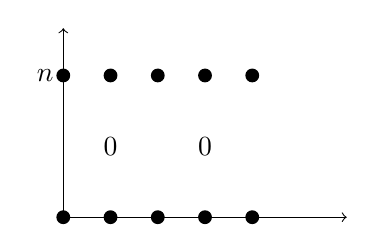
\begin{tikzpicture}[baseline=0pt, x=0.6cm, y=0.6cm]
\draw[->] (0,0) -- (0,4);
\draw[->] (0,0) -- (6,0);
\node[left] at (0,3) {$n$};
\foreach \i in {0,...,4} { \fill (\i,3) circle (2.5pt); \fill (\i,0) circle (2.5pt); }
\node at (1,1.5) {$0$};
\node at (3,1.5) {$0$};
\end{tikzpicture}
\qquad ,
\]
donc on trouve la suite exacte
\[
0 \longrightarrow H^n(Y,F) \longrightarrow H^n(X,F_X) \xrightarrow{\ \alpha\ } H^0(Y,\ \underbrace{H^n(Z,\overbrace{F_Z}^{M_Z})}_{\begin{array}{l}\scriptstyle = \ \mathrm{Hom}(\pi_n(Z,z),M)\\ \scriptstyle \text{par \texttt{[le]} th. de Hurewicz}\end{array}}\ ) \longrightarrow H^{n+1}(Y,F).
\]

\printedpage{121}
% head: A. Grothendieck : Dérivateurs, Ch. XII, Édition des Universités de Montpellier II et Paris VII

Ici je fixe un point $x$ de $X$, $Z$ désigne la fibre de $f$ en $y=f(x)$, et $M$ celle de $F$ en $y$, $M=F_y$. Le groupe $\pi_1(Y)$ y opère, d’ailleurs $\pi \overset{\text{déf}}{=} \pi_1(X,x) \simeq \pi_1(Y,y)$ aussi. Le $H^0(Y,H^n(Z,F_Z))$ peut s’interpréter, sauf erreur, comme
\[
\mathrm{Hom}_\pi(\pi_n(Z,x),M),
\]
en tenant compte de l’opération de $\pi=\pi_1(X,x)$ sur $\pi_n(Z,x)$ également. (À vérifier.) Il faut interpréter la flèche
\[
H^n(X,F_X) \longrightarrow \mathrm{Hom}_\pi(\pi_n(Z,x),M),
\]
via l’application composée \texttt{[où $z=x$, vu comme point de $Z$]}
\[
\pi_n(Z,z) \longrightarrow \pi_n(X,x) \longrightarrow H_n(X,\mathbf{Z}). \tag*{$(*)$}
\]
Si $F$ est \textit{constant} sur $Y$ (p. ex. si $Y$ \texttt{[est]} 1-connexe), donc de valeur $M$, on a les flèches canoniques
\[
H^n(X,F_X) = H^n(X,M) \longrightarrow \mathrm{Hom}(H_n(X,\mathbf{Z}),M) \longrightarrow \mathrm{Hom}(\pi_n(Z,z),M)\text{(\footnotemark[118])} \tag*{$(*')$}
\]
\footnotetext[118]{grâce à la composition avec $(*)$.}
\texttt{[lire : }$\mathrm{Hom}_\pi$\texttt{]},

\msp{page 182}
et sûrement (en dehors de toute hypothèse de type $\mathrm{b}_n$ ou autre) l’application canonique directe ‘de localisation sur $Y$’, suivi de \dots,
\[
H^n(X,F_X) \longrightarrow H^0(Y,H^n(Z,F_Z)) \longrightarrow \mathrm{Hom}_\pi(\pi_n(Z),M) \tag*{$(**)$}
\]
n’est autre que la composée des applications canoniques ci-dessus. Dans le cas actuel où on suppose $\mathrm{b}_n$, la deuxième flèche dans $(**)$ est \texttt{[un]} isomorphisme, donc la composée ‘n’est autre’ que la flèche de localisation elle-même. D’autre part $\pi_n(Z,z) \longrightarrow \pi_n(X,x)$ dans $(*)$ est nul, donc aussi $\pi_n(Z,z) \longrightarrow H_n(X,\mathbf{Z})$, donc aussi la flèche composée $(*')$ qui s’en déduit. Revenons alors à la suite exacte de Leray (page précédente), on trouve que $H^n(Y,F) \xrightarrow{\ \sim\ } H^n(X,F_X)$.

\dgrblock{dgrb544}{The exact sequence behind the cohomological implication}
\begin{dcomment}{exposition}{p181}{The exact sequence behind the cohomological implication}
The use of a path replacement now lets Grothendieck import the classical fibration argument into his categorical model. Assume $b_n$, reduce to a connected component, and replace $f$ by a fibration with fibre $Z$. Then $Z$ is $(n-1)$-connected, and the homotopy sequence also says that $\pi_nZ\to\pi_nX$ is zero. For an abelian local system $F$ on $Y$ with fibre $M$ at $y$, the restriction $F|_Z$ is constant. The cohomological Serre--Leray spectral sequence has
\[
 E_2^{p,q}=H^p(Y;\mathcal H^q(Z;M))
 \quad\Longrightarrow\quad H^{p+q}(X;f^*F).
\]
Here $\mathcal H^q(Z;M)$ includes both the transport of the fibre and that of $M$; replacing it by an untwisted constant group would lose the content of the argument. The historical spectral sequence is \citet[Chapter~II, \S8, Proposition~6]{Serre1951}; for the indexing and filtration in the untwisted presentation see \citet[Theorem~1.14]{HatcherSS2004}.

Since $H^q(Z;M)=0$ for $0<q<n$, the only contributions in total degrees at most $n$ are the bottom row and $E_2^{0,n}$. No differential reaches the bottom row before $d_{n+1}$ from $(0,n)$ to $(n+1,0)$. Reading the filtration therefore gives the natural exact sequence
\[
\begin{split}
0\longrightarrow H^n(Y;F)&\longrightarrow H^n(X;f^*F)
 \xrightarrow{\alpha}\operatorname{Hom}_{\mathbf Z[\pi]}
       (\pi_nZ,M)\\
 &\longrightarrow H^{n+1}(Y;F)
 \longrightarrow H^{n+1}(X;f^*F),
\end{split}
\]
where $\pi=\pi_1Y=\pi_1X$. Only exactness through the penultimate group is needed. The identification of $E_2^{0,n}$ uses the natural Hurewicz isomorphism $\pi_nZ\cong H_nZ$ and the universal coefficient theorem, followed by taking monodromy invariants. The fibre is simply connected, so no ambiguity from inner automorphisms survives in its degree-$n$ group. The map $\alpha$ is restriction to a fibre, viewed as an invariant homomorphism.

There is an efficient chain-level way to finish the twisted case. If $T$ is connected with fundamental group $\pi$, a local system $G$ with fibre $M$ is represented by a left $R=\mathbf Z[\pi]$-module. A cocycle representing $c\in H^n(T;G)$ is an $R$-linear map
\[
 z:C_n(\widetilde T)\longrightarrow M,
 \qquad z\partial=0.
\]
Evaluation on cycles gives a homomorphism $H_n(\widetilde T)\to M$; changing $z$ by a coboundary has zero effect on cycles. Composing with the equivariant Hurewicz homomorphism produces
\[
 \varepsilon_G:H^n(T;G)\longrightarrow
 \operatorname{Hom}_R(\pi_n(T,t),M),\qquad n\geq2.
\]
This is the desired spherical evaluation. Its additivity follows from the homomorphism property of Hurewicz, or from the pinch map of the sphere; its equivariance follows directly from $R$-linearity. Naturality follows by lifting a pointed map to universal covers and applying the chain map. The local-coefficient chain model is described in \citet[\S3H, pp.~327--334]{Hatcher2002}; the verification above supplies the particular application the manuscript leaves open.

For $j:Z\to X$, choose the lift $Z\to\widetilde X$ corresponding to the marked point. Because $Z$ is simply connected and $(n-1)$-connected, naturality of evaluation and Hurewicz identify $\alpha$ with
\[
 H^n(X;f^*F)\xrightarrow{\varepsilon_{f^*F}}
 \operatorname{Hom}_R(\pi_nX,M)
 \xrightarrow{j^*}\operatorname{Hom}_R(\pi_nZ,M).
\]
The last map is zero because $j_*:\pi_nZ\to\pi_nX$ is zero. Hence $\alpha=0$, and exactness proves that $H^n(Y;F)\to H^n(X;f^*F)$ is an isomorphism. In lower degrees it is already an isomorphism by the zero rows of the spectral sequence. Degrees $0$ and nonabelian $1$ are controlled by the fundamental groupoid. This completes $b_n\Rightarrow c_n$ for all the coefficients actually stated, without an assumption of simple connectivity.
\end{dcomment}


Comment récupérer le cas où $F$ n’est \textit{pas} constant? Dans le cas $n=2$, cela marchait, en passant aux revêtements universels $\tilde{X}$, $\tilde{Y}$ de $X$, $Y$ (par rapport aux points $x$, $y$ choisis), et en écrivant les suites spectrales
\[
\begin{tikzcd}[row sep=small, column sep=small]
H^*(Y,F) \arrow[d] & \Longleftarrow & E_2^{pq} \arrow[d] & = & H^p(\pi,H^q(\tilde{Y},F_{\tilde{Y}})) \\
H^*(X,F_X) & \Longleftarrow & E^{\prime pq}_2 & = & H^p(\pi,H^q(\tilde{X},F_{\tilde{X}})).
\end{tikzcd}
\]
L’hypothèse $\mathrm{b}_n$ est conservée en passant de $f : X \longrightarrow Y$ à $\tilde{f} = \tilde{f}_x : \tilde{X} \longrightarrow \tilde{Y}$, donc on sait que
\printedpage{122}
% head: A. Grothendieck : Dérivateurs, Ch. XII, Édition des Universités de Montpellier II et Paris VII
\msp{page 183}
\[
E_2^{pq} \xrightarrow{\ \sim\ } E^{\prime pq}_2 \qquad \text{\texttt{[est un]} isomorphisme si } q \le n. \tag*{$(*)$}
\]
Dans le cas $n=2$, utilisant que
\[
E_2^{p1} = E^{\prime p1}_2 = 0 \qquad \text{car } H^1(\tilde{X}) = H^1(\tilde{Y}) = 0, \qquad
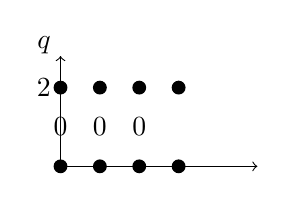
\begin{tikzpicture}[baseline=0pt, x=0.5cm, y=0.5cm]
\draw[->] (0,0) -- (0,2.8);
\draw[->] (0,0) -- (5,0);
\node[above left] at (0,2.6) {$q$};
\node[left] at (0,2) {$2$};
\foreach \i in {0,...,3} { \fill (\i,2) circle (2.5pt); \fill (\i,0) circle (2.5pt); }
\node at (0,1) {$0$};
\node at (1,1) {$0$};
\node at (2,1) {$0$};
\end{tikzpicture}
\qquad ,
\]
on trouve deux suites exactes
\[
\begin{tikzcd}
0 \arrow[r] & H^2(\pi,H^0(\tilde{Y})) \arrow[r] \arrow[d, "\text{iso}"] & H^2(Y) \arrow[r] \arrow[d] & H^0(\pi,H^2(\tilde{Y})) \arrow[r] \arrow[d, "\text{iso}"] & H^3(\pi,H^0(\tilde{Y})) \arrow[d, "\text{iso}"] \\
0 \arrow[r] & H^2(\pi,H^0(\tilde{X})) \arrow[r] & H^2(X) \arrow[r] & H^0(\pi,H^2(\tilde{X})) \arrow[r] & H^3(\pi,H^0(\tilde{X})),
\end{tikzcd}
\]
et un homomorphisme de l’une dans l’autre, qui permet de conclure par le lemme des 5 que $H^2(Y,F) \longrightarrow H^2(X,F_X)$ est \texttt{[un]} isomorphisme. Mais pour $n$ quelconque, la relation $(*)$ sur les termes $E_2$ (pour $q \le n$) ne me semble pas impliquer la relation similaire pour les $E_n$ supérieures, et de là pour les termes $E_\infty$, ce qui permettrait de conclure.

Je reviens donc à la suite exacte p. 181, avec $F$ faisceau \textit{tordu.} J’ai envie de trouver une application canonique
\[
H^n(X,G) \longrightarrow \overbrace{\mathrm{Hom}_\pi(\pi_n(X,x),G_x)}^{\text{\scriptsize Homs \textit{additifs} bien sûr, i.e. de $\mathbf{Z}[\pi]$-modules}} \qquad ,
\]
où $G$ est un faisceau abélien localement constant quelconque sur $X$, et $\pi = \pi_1(X,x)$. Si j’interprète
\msp{page 184}
$\pi_n(X,x)$ par des classes d’homotopie d’applications ponctuées
\[
(S^n,x_0) \xrightarrow{\ \varphi\ } (X,x)
\]
j’ai bien, pour une telle application $\varphi$,
\[
\varphi^* : H^n(X,G) \longrightarrow H^n(S^n,\ \overbrace{\varphi^*G}^{\simeq\,(G_x)_{S^n}}\ ) \simeq G_x
\]
(tenant compte que $S^n$ est 1-connexe, et que sa $n$-cohomologie à valeurs dans un faisceau constant $M$ est $M$.) Sûrement l’application
\[
H^n(X,G) \longrightarrow G_x
\]
\printedpage{123}
% head: A. Grothendieck : Dérivateurs, Ch. XII, Édition des Universités de Montpellier II et Paris VII
ainsi définie ne dépend que de la classe d’homotopie ponctuée de $\varphi$, d’où
\[
\pi_n(X,x) \times H^n(X,G) \longrightarrow G_x,
\]
et il faut de plus prouver a) que c’est compatible avec les opérations de $\pi = \pi_1(X,x)$, et b) que c’est additif en $\pi_n(X,x)$, pour avoir l’application cherchée
\[
H^n(X,G) \longrightarrow \mathrm{Hom}_\pi(\pi_n(X,x),G_x).
\]
Si j’admets ceci, il n’y a qu’un pas pour admettre aussi que la flèche qui nous intéresse vraiment (dans la suite exacte p. 181)
\msp{page 185}
\[
H^n(X,F_X) \longrightarrow \mathrm{Hom}_\pi(\pi_n(Z,z),\underbrace{M}_{=\,F_y})
\]
n’est autre que la composée de la flèche précédente (page précédente) pour $G = F_X$, avec
\[
\mathrm{Hom}_\pi(\pi_n(X,x),M) \longrightarrow \mathrm{Hom}_\pi(\pi_n(Z,x),M)
\]
déduite de
\[
\pi_n(Z,x) \longrightarrow \pi_n(X,x).
\]
Or cette flèche est nulle, par l’hypothèse $\mathrm{b}_n$. Donc la flèche $\alpha$ dans la suite exacte page 181 est nulle, donc $H^n(Y,F) \longrightarrow H^n(X,F_X)$ est \texttt{[un]} isomorphisme, q.e.d. (mais il y a pas mal de travail de vérification à faire \dots).

\dgrblock{dgrb545}{Completing the universal-cover comparison}
\begin{dcomment}{development}{p183}{Completing the universal-cover comparison}
Grothendieck briefly abandons the universal-cover method because he does not see how its comparison of $E_2$ rows controls later pages. The method can be completed directly at the level of complexes. It is useful to record the argument, since the needed range is finite and one should not invoke an unrestricted comparison theorem without checking its boundary. We use the ordinary truncation of complexes and the local-coefficient complex in \citet[\S3H]{Hatcher2002}. We did not find this particular completion of p.~183 in the consulted literature; its ingredients are standard homological algebra.

\textbf{Finite-range descent lemma.}\ours\ Let $\pi$ be a group and let $u:C\to D$ be a map of nonnegative cochain complexes of $\mathbf Z[\pi]$-modules which induces isomorphisms on cohomology in degrees $0\leq q\leq n$. Then
\[
 H^k(R\Gamma(\pi,C))\longrightarrow
 H^k(R\Gamma(\pi,D))
\]
is an isomorphism for $0\leq k\leq n$.

\textit{Proof.} The smart truncation $\tau_{\leq n}C$ agrees with $C$ below $n$, has $\ker(d:C^n\to C^{n+1})$ in degree $n$, and is zero above $n$. The natural inclusion fits into the truncation triangle
\[
 \tau_{\leq n}C\longrightarrow C\longrightarrow\tau_{\geq n+1}C.
\]
Derived invariants carry a complex whose cohomology vanishes below $n+1$ to one with the same lower bound. Indeed, choose an injective resolution starting in degree $n+1$, or inspect the first-quadrant spectral sequence with terms $H^p(\pi,H^q(-))$: all its potentially nonzero terms have $p\geq0$ and $q\geq n+1$. Applying $R\Gamma$ to the triangle and taking its long exact cohomology sequence shows that
\[
 H^k(R\Gamma(\pi,\tau_{\leq n}C))
 \xrightarrow{\sim}H^k(R\Gamma(\pi,C)),\qquad k\leq n,
\]
because the adjacent terms of degrees $k-1$ and $k$ for $\tau_{\geq n+1}C$ both vanish. The same holds for $D$. Finally $\tau_{\leq n}u$ is a quasi-isomorphism, and derived invariants preserve quasi-isomorphisms. The two truncation comparisons prove the assertion.\hfill$\square$

Apply the lemma to the equivariant cochain complexes of the universal covers with constant fibre $M$ and its given $\pi$-action. Derived invariants compute the cohomology with the corresponding local coefficients on the quotient: one may use a free resolution of $\mathbf Z$ over $\mathbf Z[\pi]$ and the usual total double complex. Indeed, each group of covering chains is free over $\mathbf Z[\pi]$, so each cochain term is a product of coinduced modules and is acyclic for the invariants functor. Its ordinary invariant complex is the local-coefficient cochain complex. The simply connected case of $b_n\Rightarrow c_n$ gives the required cohomology isomorphisms of the cover complexes through degree $n$, and the lemma gives the desired twisted comparison on $X$ and $Y$. Thus the alternative proposed on p.~182 does work. The spherical-evaluation proof remains closer to the geometric reason the edge map vanishes.
\end{dcomment}


$\mathrm{c}_n \Longrightarrow \mathrm{a}_{n-1}$. On peut procéder par récurrence sur $n$. (NB L’enoncé a un sens même pour $n=1$, où il est prouvé, et même $\mathrm{c}_1 \Longrightarrow \mathrm{b}_1$, et $\mathrm{b}_1 \Longrightarrow \mathrm{a}_0$, plus généralement $\mathrm{b}_n \Longrightarrow \mathrm{a}_{n-1}$, immédiat par \texttt{[la]} suite exacte d’homotopie.) Donc on sait déjà, en plus de l’hypothèse $\mathrm{c}_n$, qu’on a $\mathrm{a}_{n-2}$, i.e. $Z$ est $(n-2)$-connexe. Il faut prouver qu’il est même $(n-1)$-connexe, i.e. $\pi_{n-1}(Z)=0$. Le cas $n=2$ demande % [sic] L’enoncé -> L’énoncé, missing accent on é
\msp{page 186}
peut-être une attention particulière, car on ne sait pas même encore que $Z$ est 1-connexe. Mais on sait que $\mathrm{c}_2$ implique $\mathrm{c}_1$, qui équivaut \texttt{[?]} à $\mathrm{b}_1$, donc on a
\[
\pi_1(X,x) \longrightarrow \pi_1(Y,y) \qquad \text{isomorphisme,}
\]
donc
\[
\pi_1(Z,x) \longrightarrow \pi_1(X,x) \qquad \text{\texttt{[est]} \textit{nul,}}
\]
donc
\[
\pi_2(Y,y) \longrightarrow \pi_1(Z,x) \qquad \text{\texttt{[est un]} épimorphisme,}
\]
ce qui implique tout au moins que $\pi_1(Z,x)$ est \textit{abélien.} Il faut le voir comme un $\pi$-module, et prouver sa nullité comme tel (moyennant $\mathrm{c}_2$).

\dgrblock{dgrb546}{Recovering the first missing homotopy group}
\begin{dcomment}{exposition}{p185}{Recovering the first missing homotopy group}
For the converse direction Grothendieck changes the use of the spectral sequence: instead of annihilating the edge map, he chooses coefficients in which the first possible fibre group can test itself. This is why all local systems must be admitted. A single constant coefficient group need not detect a nontrivial module with monodromy.

Assume $c_n$. The degree-$0$ and degree-$1$ conditions give $\pi_0X=\pi_0Y$ and identify $\pi_1X$ with $\pi_1Y=\pi$. Induction gives that the homotopy fibre $Z$ is $(n-2)$-connected. For $n\geq3$ its first possible nonzero group $A=\pi_{n-1}Z$ is abelian and Hurewicz identifies it with $H_{n-1}Z$. For $n=2$ one must first justify the same assertion differently: exactness gives a surjection $\pi_2Y\twoheadrightarrow\pi_1Z$, since $\pi_1X\to\pi_1Y$ is an isomorphism. Thus $\pi_1Z$ is abelian, and its abelianization map to $H_1Z$ is already an isomorphism. In both cases transport makes $A$ a $\pi$-module; the possible ambiguity in degree one is inner conjugation in an abelian group and therefore vanishes.

For the local system determined by a $\pi$-module $M$, the first nonzero fibre row gives
\[
\begin{split}
0\longrightarrow H^{n-1}(Y;M)&\longrightarrow H^{n-1}(X;f^*M)
 \longrightarrow\operatorname{Hom}_{\mathbf Z[\pi]}(A,M)\\
 &\longrightarrow H^n(Y;M)\longrightarrow H^n(X;f^*M).
\end{split}
\]
For $n=2$, the degree-one groups in this display use abelian coefficients, a case included in $c_n$. The first comparison is surjective and the last is injective. Exactness therefore forces $\operatorname{Hom}_{\mathbf Z[\pi]}(A,M)=0$. Every $\pi$-module occurs as a coefficient system on $Y$, so take $M=A$. The identity of $A$ must vanish, and hence $A=0$. This proves $c_n\Rightarrow a_{n-1}$, with the endpoint case checked rather than hidden under an appeal to Hurewicz.

This proof uses less than full $c_n$ at its final step: after the lower-degree induction, surjectivity in degree $n-1$ and injectivity in degree $n$ suffice. The full hypothesis is a convenient uniform formulation, not an optimal list of separate tests. The source has found the correct mechanism; the qualifications about coefficients and the degree-one fibre group complete its sketch.
\end{dcomment}


\printedpage{124}
% head: A. Grothendieck : Dérivateurs, Ch. XII, Édition des Universités de Montpellier II et Paris VII

Passons au cas général. On a pour $F$ localement constant abélien sur $Y$
\[
H^*(X,F_X) \Longleftarrow \underbrace{E_2^{pq} = H^p(Y,H^q(Z,F_Z))}_{\begin{array}{l}\scriptstyle = 0 \text{ si } 0<q<n-1\\ \scriptstyle \text{car } Z \text{ est } (n-2)\text{-connexe}\end{array}}, \qquad
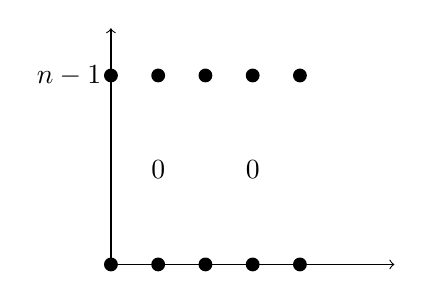
\begin{tikzpicture}[baseline=0pt, x=0.6cm, y=0.6cm]
\draw[->] (0,0) -- (0,5);
\draw[->] (0,0) -- (6,0);
\node[left] at (0,4) {$n-1$};
\foreach \i in {0,...,4} { \fill (\i,4) circle (2.5pt); \fill (\i,0) circle (2.5pt); }
\node at (1,2) {$0$};
\node at (3,2) {$0$};
\end{tikzpicture}
\qquad ,
\]
D’où
\[
0 \longrightarrow H^{n-1}(Y,F) \longrightarrow H^{n-1}(X,F_X) \longrightarrow \underbrace{H^0(Y,H^{n-1}(Z,F_Z))}_{\begin{array}{l}\scriptstyle \mathrm{Hom}_\pi(\pi_{n-1}(Z,x),F_x)\\ \scriptstyle \text{par Hurewicz}\end{array}} \longrightarrow H^n(Y,F) \longrightarrow H^n(X,F_X).
\]
L’hypothèse $\mathrm{c}_n$ implique qu’on a
\msp{page 187}
\[
\mathrm{Hom}_\pi(\pi_{n-1}(Z,x),\underbrace{M}_{=\,F_x}) = 0
\]
et ceci \textit{quel que soit le $\pi$-module $M$,} puisque $\pi = \pi_1(X,x) \xrightarrow{\ \sim\ } \pi_1(Y,y)$. Cela implique (en prenant p. ex. $M = \pi_{n-1}(Z,x)$ !) que $\pi_{n-1}(Z,x)=0$. (Mais en faisant attention, dans le cas $n=2$, qu’on sait déjà que $\pi_1(Z,x)$ est abélien).

Donc le théorème rectifie page 178 a bien l’air vrai. Il est un peu triste, puisque dans chacune des implications % [sic] rectifie -> rectifié, past participle intended
\[
\mathrm{a}_n \ \Longrightarrow\ \mathrm{b}_n \ \Longrightarrow\ \mathrm{c}_n \ \Longrightarrow\ \mathrm{a}_{n-1}
\]
on perd un chouia, et en fin de compte on sort avec la magnifique implication
\[
\mathrm{a}_n \ \Longrightarrow\ \mathrm{a}_{n-1}.
\]
De toutes façons, il est $\pm$ clair que le “bon” localiseur $W_n$, celui qui doit définir les “$n$-types d’homotopie” comme objets de $\mathrm{Hot}_{W_n}$, est défini par la condition $\mathrm{a}_n$.

\section*{2\quad Critère de $W_n$-asphéricité.}

Je vais essayer de faire mieux quand $Y$ est réduit à un point. Cette fois, je

% ---- from Der-ChXIIc-30-03-03_p011-015.tex
\printedpage{125}
% head: A. Grothendieck : Dérivateurs, Ch. XII, Édition des Universités de Montpellier II et Paris VII
% foot: Version 30 mars 2003

\msp{page 188}
veux être strict, et donner (si je peux) des démonstrations complètes dans le cadre où je me place à présent, celui du modéliseur Cat, et en n'utilisant que ce que je sais y démontrer directement à présent, sans me référer à la théorie semi-simpliciale ou topologique.

\dgrblock{dgrb547}{Degree two and the localizer correction}
\begin{dcomment}{development}{p187}{Degree two and the localizer correction}
Two brief remarks in the manuscript deserve a more precise disposition. The suggestion of a degree-two counterexample is stronger than the examples support, and the choice of the fibre condition as the localizer confuses a useful generating class with its saturation. Both can be settled without changing the successful implication arguments.

\textbf{The degree-two converse.}\ours\ For maps of classifying spaces, the condition $c_2$ implies $b_2$. Consequently $b_2$ and $c_2$ are equivalent without a simple-connectivity hypothesis.

\textit{Proof.} The degree-one argument already identifies fundamental groupoids, so work on one component and write $R=\mathbf Z[\pi]$. Let
\[
 I=\operatorname{Hom}_{\mathbf Z}(R,\mathbf Q/\mathbf Z),
 \qquad (r\varphi)(s)=\varphi(sr).
\]
This is a left $R$-module and hence a permitted local system on $Y$. Evaluation at $1\in R$ gives a natural adjunction isomorphism
\[
 \operatorname{Hom}_R(C_*(\widetilde Y),I)
 \cong\operatorname{Hom}_{\mathbf Z}
                  (C_*(\widetilde Y),\mathbf Q/\mathbf Z),
\]
and likewise for $X$. Its inverse sends a homomorphism $\lambda$ to the map $c\mapsto(r\mapsto\lambda(rc))$. Since $\mathbf Q/\mathbf Z$ is injective as an abelian group, evaluation on homology gives
\[
 H^2(Y;I)\cong
 \operatorname{Hom}_{\mathbf Z}(H_2\widetilde Y,\mathbf Q/\mathbf Z).
\]
The isomorphism is natural in the lifted map $\widetilde f$. Hypothesis $c_2$ therefore says that the dual of $H_2(\widetilde f)$ is an isomorphism. Dualization into $\mathbf Q/\mathbf Z$ is exact and detects nonzero abelian groups: a nonzero element generates a cyclic subgroup with a nonzero homomorphism to $\mathbf Q/\mathbf Z$, and injectivity extends this homomorphism to the whole group. Applying this observation to kernel and cokernel shows that $H_2(\widetilde f)$ itself is an isomorphism. The universal covers are simply connected, so the natural Hurewicz isomorphisms $\pi_2\widetilde X\cong H_2\widetilde X$ and $\pi_2\widetilde Y\cong H_2\widetilde Y$ prove that $\pi_2f$ is an isomorphism.\hfill$\square$

The algebraic ingredients are the standard injective-cogenerator argument, checked in \citet[Tags 01D8 and 08WE]{StacksInjective2026}, together with \citet[Theorem~4.32]{Hatcher2002}. We did not find a source addressing footnote~112 specifically; this is our application of those familiar tools to its question. It is not a new form of the Hurewicz theorem. The same argument shows that the degree-$j$ part of $c_n$ detects the map on $H_j$ of universal covers. For $j=2$ these homology groups are exactly $\pi_2$; for $j=3$ the Hopf class in the earlier example explains why the conclusion changes.

Now consider the last sentence of p.~187. If $A\ne0$, the maps
\[
 *\xrightarrow{s}K(A,n+1)\xrightarrow{r}*
\]
satisfy $rs=1$. The fibre of $r$ is $n$-connected and the fibre of $rs$ is contractible, but the fibre of $s$ is $K(A,n)$, which is not $n$-connected. Thus the class defined by $a_n$ fails two-out-of-three. The class defined by $b_n$, equivalently the maps made into equivalences by $n$th Postnikov truncation, is the correct weak-equivalence class for $n$-types. The modern truncation adjunction is given in \citet[Proposition~5.5.6.18]{Lurie2009HTT}.

There is a charitable precise reading of Grothendieck's intuition.

\textbf{Saturation of the fibre class.}\ours\ In spaces, $a_n$ \emph{generates} the same localization as $b_n$.

\textit{Proof.} Every Postnikov map $X\to P_nX$ has $n$-connected fibres: it is an isomorphism on $\pi_i$ through $n$, and the target has zero $\pi_{n+1}$. Given a $b_n$-map $f:X\to Y$, its natural square with $P_nf:P_nX\to P_nY$ has vertical maps in $a_n$, and its lower map is a weak homotopy equivalence, hence also lies in $a_n$. Two-out-of-three puts $f$ in the saturation of $a_n$. Conversely, $b_n$ is saturated and contains $a_n$. This proves the equality.\hfill$\square$

The proof is a direct application of the standard truncation adjunction just cited; the formulation addresses the specific localizer sentence, without a priority claim. It leaves the literal definition on p.~187 marked as false. For $X\to *$, the two conditions agree already before saturation, so the next theorem needs no change of indexing.
\end{dcomment}


\textbf{Théorème 2} (?). \textit{Soit $X$ dans} Cat, \textit{$n \in \mathbf{N}$ un entier $\geq 1$. Alors les conditions suivantes sont équivalentes :}

\begin{itemize}
\item[\textit{$a_n$)}] \textit{$X$ est $0$-connexe, et si $x$ est dans $X$, $\pi_i(X,x) = 0$ pour $i \in [1,n]$ (condition qui ne dépend pas du choix de $x$), i.e. les $\Omega^i(X,x)$ pour $i \in [1,n]$ sont $0$-connexes.}
\item[\textit{$b_n$)}] \textit{Pour tout groupe $G$, $G \longrightarrow H^0(X,G_X)$ est un isomorphisme, et $H^1(X,G_X) = 0$. De plus, si $G$ est abélien, on a aussi $H^i(X,G_X) = 0$, pour $i \in [1,n]$.}
\end{itemize}

\textsc{Démonstration}. Pour $n = 1$ cette équivalence est $\pm$ tautologique et a été rappelée (sous une forme légèrement différente) au début (p.~71). On procède par récurrence. On peut donc supposer que $n \geq 2$, que $X$ satisfait $\mathrm{a}_{n-1}$, $\mathrm{b}_{n-1}$, et prouver qu'alors $\mathrm{a}_n$, $\mathrm{b}_n$ sont équivalentes, i.e. $\pi_n(X,x) = 0$ équivaut à $H^n(X,M) = 0$ pour tout groupe abélien $M$.

\msp{page 189}
On utilise la $W_\infty$-fibration (parfaite)
\[
\begin{tikzcd}[row sep=large]
E = \Ch(X;x,-) \arrow[d] & E\ W_\infty\text{-asphérique} \\
X &
\end{tikzcd}
\]
de fibre $Z$ en $x$ égale à $\Omega(X,x)$.

\dgrblock{dgrb548}{Why the path fibration is the right final test}
\begin{dcomment}{context}{p188}{Why the path fibration is the right final test}
Grothendieck now asks the categorical path construction to reproduce an argument whose classical power came from the contractible total space of based paths. Serre's thesis developed precisely this exchange between the homology of a space, that of its loop space, and their homotopy groups; see \citet[Chapter~IV, \S5, Proposition~7]{Serre1951}. The point of repeating the argument in $\Cat$ is not a new calculation of the groups. It is to show that the categorical paths already carry enough geometry to recognize the ordinary weak homotopy type, before appealing to a comparison with topological paths.

For $E=\Ch(X;x,-)\to X$, the total category is $W_\infty$-aspherical and the fibre is $Z=\Omega(X,x)$. Under the induction hypothesis, both base and fibre have long vanishing ranges. The spectral sequence then has only its bottom row and one possible first fibre row. The vanishing of the total cohomology forces those two rows to communicate by transgression. This is the reason the proof over a point is sharper than the preceding relative theorem: there is no independent cohomology of a nontrivial target that can absorb the first obstruction.

The condition in degree zero should be read literally for every group. Taking a nontrivial group $G$, the diagonal map $G\to G^{\pi_0X}$ is bijective only when $\pi_0X$ has one element. It excludes the empty category as well. Once $X$ is connected, the condition $H^1(X,G_X)=*$ for every group $G$ forces $\pi_1X=1$: choose $G=\pi_1X$ and the conjugacy class of its identity representation. This is why abelian coefficients alone would not prove the initial case; a perfect nontrivial fundamental group could otherwise survive.
\end{dcomment}


Supposons $\mathrm{a}_n$) pour $X$, donc $a_{n-1}$) pour $\Omega(X,x)$. Par hypothèse de récurrence, on a donc
\[
H^i(Z,M) = 0 \qquad \text{pour } i \in [1,n-1],
\]
$M$ groupe abélien. Donc dans la suite spectrale de Leray,
\[
H^*(E,M) \Longleftarrow E_2^{pq} = H^p(X,H^q(Z,M))
\]
on a
\[
E_2^{pq} = 0 \qquad \text{si } q \in [1,n-1], \qquad
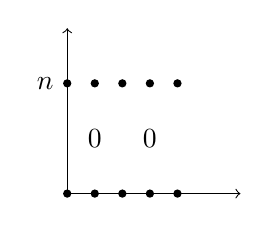
\begin{tikzpicture}[baseline=0]
\draw[->] (0,0) -- (2.2,0);
\draw[->] (0,0) -- (0,2.1);
\foreach \x in {0,0.35,0.7,1.05,1.4} {
  \fill (\x,0) circle (1.5pt);
  \fill (\x,1.4) circle (1.5pt);
}
\node[left] at (-0.05,1.4) {$n$};
\node at (0.35,0.7) {$0$};
\node at (1.05,0.7) {$0$};
\end{tikzpicture}
\quad .
\]

\printedpage{126}
% head: A. Grothendieck : Dérivateurs, Ch. XII, Édition des Universités de Montpellier II et Paris VII
% foot: Version 30 mars 2003

On a donc la suite exacte
\[
0 \longrightarrow H^n(X,M) \longrightarrow H^n(E,M)
\]
et comme $E$ est $W_\infty$-asphérique, on a $H^n(E,M) = 0$, donc $H^n(X,M) = 0$.

Inversement, supposons $\mathrm{b}_n$), prouvons $\mathrm{a}_n$). On sait déjà qu'on a $\mathrm{a}_{n-1}$), donc $\mathrm{a}_{n-2}$ pour $\Omega(X,x)$, ce qui implique
\[
H^i(Z,M) = 0 \qquad \text{pour } i \in [1,n-2],
\]
donc
\[
E_2^{pq} = 0 \qquad \text{si } q \in [1,n-2].
\]
On a donc la suite exacte

\msp{page 190}
\[
0 \longrightarrow \underbrace{H^{n-1}(X,M)}_{=\,0} \longrightarrow \underbrace{H^{n-1}(E,M)}_{=\,0} \longrightarrow H^0(X,H^{n-1}(Z,M)) \longrightarrow \underbrace{H^n(X,M)}_{=\,0} \longrightarrow H^n(E,M),
\]
donc
\[
H^0(X,\ \underbrace{H^{n-1}(Z,M)}_{\begin{array}{l}\text{système local}\\ \textit{constant}\text{ sur } X,\\ \text{car } X \text{ est 1-connexe}\end{array}}\ ) = 0,
\]
donc
\[
H^{n-1}(Z,M) = 0,
\]
ce qui, par hypothèse de récurrence, implique $\pi_{n-1}(Z,z) = 0$, donc $\pi_n(X,x) = 0$, q.e.d.

\textbf{Corollaire.} \textit{Pour que $X$ soit $W_\infty$-asphérique, i.e. pour qu'on ait $G \xrightarrow{\ \sim\ } H^0(X,G)$, $H^1(X,G) = 0$} \texttt{[pour]} \textit{tout groupe} \texttt{[}$G$\texttt{]}\textit{, et $H^i(X,G) = 0$ si $i \geq 2$ pour $G$ abélien, il faut et il suffit que} $1^\circ$) \textit{$X$ soit} $0$\textit{-connexe, et ($x$ étant un point de $X$)} $2^\circ$) \textit{les $\Omega^i(X,x)$} \texttt{[soient]} $0$\textit{-connexes pour $i \geq 1$.}

\msp{page 191}

\dgrblock{dgrb549}{The loop criterion, including its degree-two endpoint}
\begin{dcomment}{exposition}{p190}{The loop criterion, including its degree-two endpoint}
Theorem~2 is proved by the displayed induction, with one small verification at its lower endpoint. Suppose first that $X$ is $n$-connected. Then $Z=\Omega X$ is $(n-1)$-connected, so the induction hypothesis annihilates $H^q(Z;M)$ for $1\leq q<n$. In the path-fibration spectral sequence this gives an injection
\[
 H^n(X;M)\hookrightarrow H^n(E;M)=0.
\]
The lower-degree groups have already vanished, and the degree-zero and torsor conditions follow from connectedness and simple connectivity. This proves the forward implication exactly in the form stated.

Conversely, assume the cohomological conditions through degree $n$. The induction hypothesis makes $X$ $(n-1)$-connected and $Z$ $(n-2)$-connected. For $n\geq2$, $X$ is simply connected, so the fibre-cohomology local systems on $X$ are constant. The low-degree exact sequence for $E\to X$ gives
\[
 H^0(X;\mathcal H^{n-1}(Z;M))=0,
 \qquad\text{hence}\qquad H^{n-1}(Z;M)=0
\]
for every abelian $M$. If $n\geq3$, $Z$ is simply connected. Its nonabelian degree-one conditions and all its lower abelian cohomology conditions are already satisfied; the induction hypothesis applied to $Z$ therefore gives $\pi_{n-1}Z=0$.

For $n=2$, one cannot immediately apply that same sentence: $Z$ is only known to be connected, and the displayed computation gives vanishing of $H^1(Z;M)$ only for abelian groups $M$. The loop multiplication supplies the missing information. The two compositions of loops in the connected loop space, concatenation of based loops and the multiplication induced from the loop-space multiplication, have the same unit and satisfy the interchange law. The Eckmann--Hilton argument makes $\pi_1Z$ abelian. Thus
\[
 H^1(Z;M)=\operatorname{Hom}(\pi_1Z,M),
\]
and choosing $M=\pi_1Z$ forces $\pi_1Z=0$. Equivalently, this is the familiar fact that $\pi_1\Omega X=\pi_2X$ is abelian. It closes the induction without requiring an additional theorem about nonabelian cohomology of $Z$.

The corollary follows by allowing every finite $n$. Connectedness of $X$ together with connectedness of every iterated loop category says that all homotopy groups of $BX$ vanish. Since a realization of a nerve has CW type, Whitehead's theorem makes $BX$ weakly equivalent, indeed homotopy equivalent, to a point; see \citet[Theorem~4.5]{Hatcher2002}. Here ``aspherical'' means weakly contractible, not merely the modern usage $\pi_i=0$ for $i>1$. For example $B\mathbf Z\simeq S^1$ has no higher homotopy groups, but its first loop category has components indexed by $\mathbf Z$, so it fails this criterion immediately.

The later minimal-localizer theorem identifies this test with Grothendieck's original axiomatic weak equivalences. Its local characterization also makes the loop method visible in the final proof: \citet[Theorem~2.3.6, especially 2.3.6.3--2.3.6.4]{Cisinski2004Minimal} passes from a weakly aspherical object to its loops and then uses vanishing of homotopy groups. Thus the categorical construction has reached its intended target. The distinction between different choices of categorical paths has become a question of canonical comparison, which is exactly the subject of the following pages.
\end{dcomment}


\section*{3\quad Sur la philosophie des fibres homotopiques.}

Le critère d'asphéricité (pour $W_\infty$) que je viens d'obtenir, grâce aux foncteur $\Ch(X)$ (ou au choix, $\Ch_\infty(X)$) et ses dérivés $\Omega(X,x)$ et les itérés, enlève tout doute (s'il pouvait en rester encore) que les `espaces de chemins' que j'ai construit (assez péniblement!) sont bel et bien `les bons'. Je voudrais maintenant me rendre compte de façon la plus précise possible de leur `canonicité', dans quelle mesure ces constructions sont indépendant d'un choix (p.ex. celui entre la théorie $\Ch$, et $\Ch_\infty$). % [sic] aux foncteur -> au foncteur, number agreement

Tout revient, finalement, à des questions de factorisation d'une flèche quelconque
\[
f : X \longrightarrow Y
\]
\printedpage{127}
% head: A. Grothendieck : Dérivateurs, Ch. XII, Édition des Universités de Montpellier II et Paris VII
% foot: Version 30 mars 2003
de Cat en
\[
X \xrightarrow{\ i_f\ } \bar{X} \xrightarrow{\ \bar{f}\ } Y,
\]
avec
\[
i_f \in W, \qquad \bar{f} \in W\text{-fib}
\]
(le fait que $\bar{f}$ puisse même être choisie $W_\omega$-parfait, ne me paraissant pas essentiel ici).

C'est bien de cela qu'il s'agit pour construire

\msp{page 192}
un objet `chemins dans $X$'
\[
\Ch(X),
\]
en factorisant l'application diagonale
\[
X \xrightarrow{\ \mathrm{diag}_X\ } X \times X,
\]
et aussi quand on construit $\Omega(X,x)$ comme fibre en $x$ d'une $W$-fibration
\[
E(X,x) \longrightarrow (X,x)
\]
qui factorise l'inclusion
\[
\{x\} \longrightarrow X
\]
(donc $E(X,x)$ étant $W$-asphérique).

\dgrblock{dgrb550}{From a model for paths to an intrinsic operation}
\begin{dcomment}{context}{p191}{From a model for paths to an intrinsic operation}
The question of canonicity belongs to Grothendieck's original reason for introducing derivators. In \emph{Pursuing Stacks}, \S69, he recalls the inadequacy of a single derived category for some of the diagrammatic constructions arising from the SGA~5 trace formalism. He proposes retaining derived categories for all diagram shapes, with their variance in the indexing category. The two three-object shapes for spans and cospans already encode homotopy fibres and cofibres \citep[\S69, printed pp.~1--3]{Grothendieck1983}. The move on these pages, from a particular category of paths to a property of localized slices, is a local instance of that larger programme.

The letter to Thomason of 2 April 1991 makes the distinction especially explicit. Its first numbered discussion treats $W$ as the essential homotopical datum and fibrations or cofibrations as additional means of proving existence and calculating operations; it then describes the intrinsic class of pullback-preserving $W$-fibrations \citep[point~1, pp.~3--4]{Grothendieck1991Letter}. This is a retrospective clarification of the position being explored here, not evidence that every provisional axiom of the present pages has already been checked. In particular, the retract qualification discussed below remains necessary under the literal two-out-of-three assumptions. The calculation of paths serves the intrinsic operation by providing enough useful representatives on which the operation becomes ordinary pullback.
\end{dcomment}


On peut être plus ou moins exigeant, et regarder, soit pour un `but' $Y$ (ou plutôt un $S$) fixé dans Cat, une factorisation fonctorielle
\[
C : \Cat/S \longrightarrow \Fib_W S \hookrightarrow \Cat/S
\]
du morphisme structural $X \longrightarrow S$ d'un objet, en
\[
X \xrightarrow{\ i_X\ } C(X) \longrightarrow S,
\]
i.e. on se donne le foncteur $C$, \textit{plus}

\msp{page 193}
le morphisme fonctoriel
\[
i_C : \mathrm{id}_{\Cat/S} \longrightarrow C
\]
avec
\[
(i_X : X \longrightarrow C(X)) \in W \qquad \forall\ X \text{ dans } \Cat/S,
\]
soit être encore plus exigeant et faire varier en même temps la source et le but de $f : X \longrightarrow Y (= S)$, et demander un foncteur
\[
\begin{aligned}
C : \Fl(\Cat) \quad &\longrightarrow \quad \Cat \\
f \quad &\longmapsto \quad C(f),
\end{aligned}
\]
\printedpage{128}
% head: A. Grothendieck : Dérivateurs, Ch. XII, Édition des Universités de Montpellier II et Paris VII
% foot: Version 30 mars 2003
avec des morphismes fonctoriels en $f$
\[
\underbrace{s(f)}_{=\,X} \xrightarrow{\ i_f\ } \underbrace{C(f)}_{=\,\bar{X}} \xrightarrow{\ p_f\ } \underbrace{b(f)}_{=\,Y}
\]
($i$, $p$ des flèches dans $\Hom(\Fl(\Cat),\Cat)$), avec
\[
i_f \in W, \qquad p_f \in W\text{-fib}
\]
pour toute flèche $f$ dans Cat.

\dgrblock{dgrb551}{A replacement must remember its comparison map}
\begin{dcomment}{exposition}{p192}{A replacement must remember its comparison map}
Grothendieck now asks what the lengthy construction of paths has bought him beyond a convenient calculation. The preceding connectivity criterion identifies its homotopical effect; it does not yet identify the construction independently of its presentation. The change of viewpoint is to regard a path category as a factorization of a structural map. A factorization of the diagonal gives paths, and a factorization of a point inclusion gives based paths. Once the second factor has the required base-change property, its ordinary fibres can serve as homotopy fibres. The same question can therefore be asked without mentioning intervals or zigzags.

For a fixed base put $\mathcal A=\Cat/S$, and let $\mathcal F\subseteq\mathcal A$ be the full subcategory of the permitted fibrations over $S$. The data are a functor $C:\mathcal A\to\mathcal F$ and a natural transformation $i:\id_{\mathcal A}\to jC$, where $j$ is inclusion and every $i_X$ belongs to $W_S$. The transformation is part of the data. An arbitrary choice of an equivalent object for every $X$ would neither provide the arrows $C(f)$ nor specify which comparison is to be called canonical. Naturality supplies both controls at once. Indeed,
\[
 C(f)i_X=i_Yf
\]
and two-out-of-three show that $f\in W_S$ if and only if $C(f)\in W_S$. Thus the homotopicality of $C$ is a consequence of its coaugmentation, not an extra axiom.

There are two levels of functoriality in the text. A replacement on $\mathcal A$ controls variation of the object over one base. A replacement on the arrow category also controls maps between bases, although it need not commute with ordinary pullbacks. The latter distinction matters: a functorial factorization of arrows does not, merely by being functorial, identify $C(X\times_S T)$ with $C(X)\times_S T$. Derived base change will be obtained from a localization argument. It is not asserted to be an identity between these raw constructions.

This is the same elementary geometry that underlies Brown's mapping-path factorization. In a category of fibrant objects, a factorization of the diagonal of $Y$ yields a factorization of $f:X\to Y$ by pulling that path object back along $f$. Brown requires no functorial choice of path objects for this argument \citep[Part I, \S1, pp.~420--422]{Brown1973}. Grothendieck deliberately asks for a more explicit choice here so that comparison maps can be written in the original category. The two approaches answer different parts of the same problem: existence of the derived construction and a convenient formula for computing it.
\end{dcomment}


\msp{page 194}
Dans les deux points de vue, dans quel sens a-t-on \textit{unicité} d'une telle construction?

Prenons d'abord le premier point de vue, factorisation des flèches à but fixé $S$, donc \texttt{[c'est une]} question dans $\Cat/S$. J'ai oublié une propriété importante, mais elle résulte de ce qui a été dit : le foncteur
\[
\begin{tikzcd}[column sep=small]
X \longmapsto C(X) : & \Cat/S \arrow[rr] \arrow[dr, dotted] & & \Cat/S \\
& & \Fib_W S \arrow[ur, dotted, hook] &
\end{tikzcd}
\]
\textit{transforme} \texttt{[les]} \textit{flèches} \texttt{[de]} \textit{$W$ en itou}, comme on voit sur le diagramme commutatif
\[
\begin{tikzcd}[row sep=large, column sep=large]
X \arrow[r, "i_X"] \arrow[d, "f"'] & C(X) \arrow[d, "C(f)"] \\
Y \arrow[r, "i_Y"] & C(Y),
\end{tikzcd}
\]
où $i_X$, $i_Y$ sont dans $W$, donc
\[
f \in W \qquad \Longleftrightarrow \qquad C(f) \in W.
\]
Soit
\[
(C',i')
\]
un deuxième foncteur, $\Cat/S \longrightarrow \Cat/S$,

\msp{page 195}
muni d'un morphisme
\[
i' : \mathrm{id}_{\Cat/S} \longrightarrow C'
\]
qui est dans $W$ argument par argument, et tel que $C'$ se factorise par $\Fib_W S$. On peut comparer $C$ et $C'$ moyennant $C \circ C'$, car
\[
\begin{tikzcd}[column sep=small]
& C \circ C' & \\
C = C \circ \mathrm{id} \arrow[ur, "C\ast i'"] & & C' = \mathrm{id} \circ C', \arrow[ul, "i\ast C'"']
\end{tikzcd}
\]
\printedpage{129}
% head: A. Grothendieck : Dérivateurs, Ch. XII, Édition des Universités de Montpellier II et Paris VII
% foot: Version 30 mars 2003
i.e. on a, pour tout $X$ dans $\Cat/S$,
\[
\begin{tikzcd}[column sep=small]
& C(C'(X)) & \\
C(X) \arrow[ur, "C(i'_X)"] & & C'(X), \arrow[ul, "i_{C'(X)}"']
\end{tikzcd}
\]
le deux flèches étant dans $W$ (celle de gauche parce que $C(W) \subseteq W$). Ce sont des flèches dans $\Fib_W S$, et si on suppose que $W$ satisfait W(4b), elles induisent des $W$-équivalences en chaque fibre. Cela montre donc déjà % [sic] le deux flèches -> les deux flèches, typo

\msp{page 196}
qu'à isomorphisme (peut-être non-canonique) près, le foncteur composé défini par $C$,
\[
\begin{tikzcd}
X \arrow[r, mapsto] & C(X) \arrow[r, mapsto] & (s \longmapsto \mathrm{hot}_W(C(X)_s)) \\
\Cat/S \arrow[r] \arrow[rr, bend right, "\varphi_C"'] & \Fib_W S \arrow[r] & \Hom(S^\circ,\mathrm{Hot}_W),
\end{tikzcd}
\]
ne dépend pas du choix particulier de $C$, i.e. deux tels foncteurs `fibres homotopiques' (correspondant à deux choix $C$, $C'$) sont toujours isomorphes. Mais au lieu d'utiliser $C \circ C'$ pour définir un tel isomorphisme, on aurai pu utiliser $C' \circ C$, ou quelque autre procédé. On aimerait comprendre s'il y a unicité véritable, une caractérisation intrinsèque de ces isomorphismes $\varphi_C \xrightarrow{\ \sim\ } \varphi_{C'}$, indépendamment de telle construction ou de telle autre. % [sic] aurai pu -> aurait pu, typo

Je présume que $C \circ C'$ est lui aussi muni de
\[
\mathrm{id}_{\Cat/S} \longrightarrow C \circ C',
\]

\msp{page 197}
et même a priori de deux façons possible
\[
\begin{tikzcd}[column sep=large, row sep=large]
& C(C'(X)) & \\
C(X) \arrow[ur, "C(i'_X)"] & & C'(X) \arrow[ul, "i_{C'(X)}"'] \\
& X, \arrow[ul, "i_X"] \arrow[ur, "i'_X"'] \arrow[uu, dotted] &
\end{tikzcd}
\]
soit par $C(i'_X) \circ i_X$, soit par $i_{C(X)} \circ i'_X$, heureusement elles sont égales, car pour toute flèche $X \xrightarrow{\ i'\ } X'$ dans $\Cat/S$, le carré % [sic] i_{C(X)} -> i_{C'(X)}, the diagram above has i_{C'(X)}

\dgrblock{dgrb552}{Two replacements and one normalized comparison}
\begin{dcomment}{exposition}{p196}{Two replacements and one normalized comparison}
The composite replacement is a useful device because it compares two constructions without asking either to map directly to the other. Write the two coaugmentations as $i:\id\to C$ and $i':\id\to C'$. For every $X$ the diagram gives
\[
 C(X)\xrightarrow{C(i'_X)}CC'(X)
       \xleftarrow{i_{C'(X)}}C'(X).
\]
Both arrows are weak equivalences: the first because $C$ preserves $W_S$, and the second because it is a component of $i$. Their passage to fibrewise equivalences uses the additional fibre axiom invoked in the text. This last step must be retained. A weak equivalence of total objects over a base need not induce weak equivalences of their ordinary fibres when the objects have not been suitably replaced.

There is already a precise answer to the question about the order $CC'$ versus $C'C$. Let $q:\mathcal A\to\mathcal A[W_S^{-1}]$ be localization. The required comparison between the two localized endofunctors is
\[
 \theta_{C,C'}(X)=q(i'_X)q(i_X)^{-1}.
\]
It is the unique comparison compatible with the specified maps from $q(X)$. Naturality of $i$, applied to $i'_X$, gives
\[
 C(i'_X)i_X=i_{C'(X)}i'_X.
\]
After localization this proves
\[
 q(i_{C'(X)})^{-1}q(C(i'_X))
       =q(i'_X)q(i_X)^{-1}.
\]
The common-refinement construction therefore gives exactly the normalized comparison. Reversing the order of the replacements gives the same answer. For three replacements the cocycle identity is literal:
\[
 \theta_{C',C''}\theta_{C,C'}=\theta_{C,C''}.
\]
The apparent ambiguity disappears as soon as compatibility with the coaugmentations is made explicit.

When this calculation is transported to the category of fibres, one uses the full faithfulness of the localization comparison proved below. In that category the formula is not an instruction to apply an ordinary fibre functor to $i_X$: its source $X$ need not be fibrant. Instead, it characterizes the comparison after passing through the equivalence of localized categories. This is the categorical content of the word ``canonical'' here. It does not say that the underlying functors admit no other automorphisms after their specified comparison maps have been forgotten.
\end{dcomment}


% ---- from Der-ChXIIc-30-03-03_p016-020.tex
\printedpage{130}
% head: A. Grothendieck : Dérivateurs, Ch. XII, Édition des Universités de Montpellier II et Paris VII

\[
\begin{tikzcd}[column sep=small, row sep=small]
 & C(X') & \\
C(X) \arrow[ur, "C(i')"] & & X' \arrow[ul, "i_{X'}"'] \\
 & X \arrow[ul, "i_X"] \arrow[ur, "i'"'] &
\end{tikzcd}
\]

est commutatif (par fonctorialité de $i_X : X \longrightarrow C(X)$), et on applique ceci au cas de $X' = C'(X)$, $i' = i'_X$.

Cette remarque nous encourage à faire un saut dans l'abstraction, et d'introduire la catégorie\msp{page 198}
\[
\mathcal{C} = \mathcal{C}_S = \begin{cases}
\text{catégorie des couples } (C,i), \text{ avec} \\
C : \Cat/S \longrightarrow \Cat/S \text{ se factorisant par } \Fib_W S, \\
i : \id_{\Cat/S} \longrightarrow C \text{ tel que } i_X \in W \ \forall\ X \text{ dans } \Cat/S,
\end{cases}
\tag*{$(*)$}
\]
une flèche
\[
(C,i) \longrightarrow (C',i')
\]
étant une flèche
\[
C \xrightarrow{u} C' \qquad \text{(dans } \Hom(\Cat/S, \Cat/S))
\]
rendant commutatif le carré \texttt{[lire : le diagramme]}
\[
\begin{tikzcd}[column sep=small]
 & \id_{\Cat/S} \arrow[dl, "i"'] \arrow[dr, "i'"] & \\
C \arrow[rr, "u"] & & C'.
\end{tikzcd}
\]

En d'autres termes, $\mathcal{C}$ est défini comme une sous-catégiorie pleine de % [sic] sous-catégiorie -> sous-catégorie, misspelled word
\[
\id_{\Cat/S}\backslash\Hom(\Cat/S, \Cat/S),
\]
à savoir celle dont les objets $(C,i)$ satisfont les deux conditions $(*)$ plus haut (impliquant l'une et l'autre le localiseur $W$).

\msp{page 199}Ces conditions impliquent ceci

\begin{enumerate}
\item[a)] $\forall\ X$ dans Cat/$S$, $(u_X : C(X) \longrightarrow C'(X)) \in W$, puisque
\[
\begin{tikzcd}[column sep=small]
 & X \arrow[dl, "i_X\in W"'] \arrow[dr, "i'_X\in W"] & \\
C(X) \arrow[rr, "u_X"] & & C'(X),
\end{tikzcd}
\]
\printedpage{131}
% head: A. Grothendieck : Dérivateurs, Ch. XII, Édition des Universités de Montpellier II et Paris VII
et

\item[b)] si $W$ satisfait W(4b), de sorte que $u_X \in W^{\mathrm{f}}_S$, alors ce définit un \textit{isomorphisme} entre $\varphi_C(X)$ et $\varphi_{C'}(X)$ % [sic] ce définit -> ceci définit, missing word
\[
\begin{tikzcd}[row sep=small]
s \arrow[r, mapsto] & \hot_W(C(X)_s) \arrow[d, "\wr\, u_{X,s}"] \\
s \arrow[r, mapsto] & \hot_W(C'(X)_s).
\end{tikzcd}
\]
\end{enumerate}

Mieux encore, dans ce cas, le foncteur composé
\[
\mathcal{C} \times \Cat/S \longrightarrow \Fib_W S \longrightarrow \HOT^{\mathrm{lc}}_W(S)
\]
donne naissance à
\[
\mathcal{C} \longrightarrow \Hom(\Cat/S, \HOT^{\mathrm{lc}}_W(S))
\]
qui transforme toute flèche de $\mathcal{C}$ en \texttt{[un]} \textit{isomorphisme,} donc se factorise par le groupoïde fondamental de $\mathcal{C}$,
\[
\Pi\mathcal{C} \longrightarrow \Hom(\Cat/S, \HOT^{\mathrm{lc}}_W(S)).
\]

\msp{page 200}Quant au foncteur envisagé tantôt
\[
\begin{aligned}
\mathcal{C} &\quad\longrightarrow\quad \underbrace{\Hom\,(\Cat/S, \Hom(S^\circ, \Hot_W))}_{\simeq\Hom((\Cat/S)\times S^\circ, \Hot_W)} \\
C &\quad\longmapsto\quad ((X,s) \longmapsto \hot_W(C(X)_s))\,,
\end{aligned}
\]
il se déduit du précédent en composant avec
\[
\begin{tikzcd}[column sep=small]
\HOT_W(S) \arrow[rr] \arrow[dr, dotted] & & \Hom(S^\circ, \Hot_W), \\
 & \Hom(\Pi S^\circ, \Hot_W) \arrow[ur, dotted] &
\end{tikzcd}
\]
plus exactement, avec le foncteur qui s'en déduit
\[
\Hom(\Cat/S, \HOT_W(S)) \longrightarrow \Hom(\Cat/S, \Hom(S^\circ, \Hot_W)).
\]

On voit poindre ici un principe plausible de canonicité d'isomorphismes, en ce qui concerne les foncteurs
\[
C_W : \Cat/S \longrightarrow \HOT^{\mathrm{lc}}_W(S)
\]
définis par les $C \in \mathrm{Ob}\,\mathcal{C}$, par la relation
\[
\Pi\mathcal{C} \approx \ \text{catégorie ponctuelle, i.e. } \mathcal{C} \text{ est 1-connexe.}
\]

De plus, les arguments utilisés jusqu'ici sont de nature à tel point formelle, que les aspects spécifiques du Modéliseur Cat
\printedpage{132}
% head: A. Grothendieck : Dérivateurs, Ch. XII, Édition des Universités de Montpellier II et Paris VII
\msp{page 201}semblent n'y jouer pratiquement aucun rôle, ou un rôle très effacé.

\dgrblock{dgrb553}{The category of choices is contractible}
\begin{dcomment}{exposition}{p200}{The category of choices is contractible}
Grothendieck's category $\mathcal C$ packages the compatibility just used. Its arrows are natural transformations of replacement functors that commute with their coaugmentations. Every such arrow is pointwise in $W_S$, by two-out-of-three. Hence any construction which sends these weak equivalences to isomorphisms factors through $\Pi\mathcal C$. The remaining question is whether this groupoid has exactly one arrow between any two objects. The natural common refinements give more: provided a replacement exists, the nerve of $\mathcal C$ is contractible.

Here is a direct proof. Fix $(R,r)\in\mathcal C$ and define
\[
 T(C,i)=\bigl(CR,(Cr)i\bigr).
\]
The displayed unit is also $(iR)r$, by naturality of $i$. The composite $CR$ takes values in $\mathcal F$, and its coaugmentation is a weak equivalence. Thus $T$ is an endofunctor of $\mathcal C$. On an arrow $u:C\to D$ put $T(u)=uR$. There are natural transformations
\[
 \id_{\mathcal C}\xrightarrow{\alpha}T
       \xleftarrow{\beta}\operatorname{const}_{(R,r)},
 \qquad \alpha_C=Cr,\quad\beta_C=iR.
\]
Both are arrows under the identity functor because $(Cr)i=(iR)r$. To check their naturality, use, respectively, naturality of $u$ at $r_X$ and the equation $ui=j$ for a map $(C,i)\to(D,j)$. These are equalities before localization.

A natural transformation $F\to G$ gives a functor $\mathcal D\times[1]\to\mathcal E$, hence a homotopy between the maps of nerves induced by $F$ and $G$; this is the elementary nerve calculation used in \citet[\S1, Proposition~2]{Quillen1973}. The two transformations above consequently homotope the identity of $|N\mathcal C|$ to a constant map. With the usual change of universe if necessary, $|N\mathcal C|$ is contractible. In particular, $\Pi\mathcal C$ is equivalent to the terminal groupoid. Any two zigzags of comparisons between the same replacements induce the same isomorphism in a target in which all arrows of $\mathcal C$ become invertible.

This argument also locates the imprecision in the word \emph{filtrante} on the next page. A common target for two objects is only one of the conditions for a filtered category; parallel arrows must also become equal after postcomposition. The common-refinement square does not establish that second condition. Nor do the natural maps into a binary product, even with all the displayed coherence, establish it in general. For example, the category of nonempty finite ordered sets and order-preserving injections has ordered concatenation and natural inclusions from both factors. It is not filtered: the two injections from a singleton into a two-element ordered set remain distinct after every injection. Nevertheless its nerve is contractible by the same argument. This example refutes the inference being used, not a separately proved assertion that this particular $\mathcal C$ fails to be filtered. Contractibility supplies precisely the canonicity needed here, so no strict equalization claim is required.
\end{dcomment}


Le carré de la page 197 montre surtout que la catégorie $\mathcal{C}$ est filtrante - $(C,i)$, $(C,i')$ s'envoient l'un et l'autre dans $(C'',i'')$, avec $C'' = C \circ C'$, et $i'' = (C * i') \circ i = (i * C') \circ i'$. Il y a même une loi de composition dans $\mathcal{C}$, nullement commutative ni unitaire c'est sûr, mais sûrement associative, et (si cette composition est notée $*$) avec des morphismes fonctoriels % [sic] (C,i') -> (C',i'), the second couple of the following formula is (C',i')
\[
\xi \xrightarrow{\alpha_{\xi,\xi'}} \xi * \xi' \xleftarrow{\beta_{\xi,\xi'}} \xi'
\]
qui assurent le caractère filtrant croissant de $\mathcal{C}$. Ces flèches semblent remplacer en quelque sorte l'unité bilatère absente, et on s'attend à ce qu'elles aient les mêmes excellentes propriétés que si on avait une telle unité, concernant les composés doubles $(\xi * \xi') * \xi'' \simeq \xi * (\xi' * \xi'')$,

\msp{page 202}
\[
(\xi * \xi') * \xi'' \xrightarrow{\sim} \xi * (\xi' * \xi'').
\]

Il y a deux façons d'envoyer un produit binaire
\[
\xi * \xi', \qquad \xi' * \xi'', \qquad \xi * \xi''
\]
dans le produit ternaire, et bien elles doivent dans chacun des trois cas, être égales. Et de même il y a, ceci admis, encore deux façons d'envoyer $\xi$ dans le produit ternaire, en factorisant soit par $\xi * \xi'$, soit par $\xi * \xi''$, et de même pour les deux autres foncteurs $\xi'$, $\xi''$; et là encore, ces deux façons doivent être égales, dans chacun de ces trois cas - donc $3 + 3 = 6$ égalités en tout à écrire et à vérifier - on a vu pire!

La philosophie calculatoire devrait être celle-ci : Si on a un produit $n$-uple
\[
\xi_1 * \xi_2 * \cdots * \xi_n
\]
(où je me dispense de mettre des parenthèses \dots), pour tout produit $m$-uple partiel $(m \in [1, n-1])$\msp{page 203}
\[
\xi_{i_1} * \xi_{i_2} * \cdots * \xi_{i_m} \qquad\qquad (i_1 < i_2 < \cdots < i_m),
\]
en utilisant à tour de bras les isomorphismes d'associativité et les $\alpha_{\xi,\xi'}$, $\beta_{\xi,\xi'}$, il n'y a pourtant qu'une seule façon de l'envoyer dans le produit $n$-uple. J'ai bien l'impression que ça doit être vrai. (Est-ce que ça implique déjà que $\mathcal{C}$ est 1-connexe?)

En fait, il y a bien une unité bilatère, mais elle n'est pas dans $\mathcal{C}$, mais dans la catégorie plus grande
\[
\id_{\Cat/S}\backslash\Hom(\Cat/S, \Cat/S),
\]
qui elle, comme toute catégorie
\[
\id_{\mathcal{X}}\backslash\Hom(\mathcal{X}, \mathcal{X}),
\]
\printedpage{133}
% head: A. Grothendieck : Dérivateurs, Ch. XII, Édition des Universités de Montpellier II et Paris VII
est une catégorie monoïdale, i.e. avec produit associatif \textit{et} unitaire. Les flèches $\alpha_{\xi,\xi'}$, $\beta_{\xi,\xi'}$ sont les flèches qui résultent de la présence de cette unité (vu que $\mathcal{C}$ est une sous-catégorie pleine), et alors il doit devenir clair qu'on a les compatibilités dites.

\msp{page 204}Mais même une catégorie monoïdale, est elle 1-connexe? Par exemple $B_G$, pour $G$ un groupe disons, est bien une catégorie monoïdale et même ‘groupale’, une $G$-catégorie (tout ce qu'il y a de strict), et pourtant elle n'est \textit{pas} 1-connexe!

\dgrblock{dgrb554}{Insertion of units accounts for all six equalities}
\begin{dcomment}{exposition}{p203}{Insertion of units accounts for all six equalities}
The associativity discussion is an effort to make the comparison procedure usable without remembering a particular sequence of refinements. It can be completed inside the ordinary monoidal category of endofunctors. An object of the coslice $\id_{\mathcal A}\backslash\operatorname{Fun}(\mathcal A,\mathcal A)$ is a pointed endofunctor $(C,i)$. Set
\[
 (C,i)*(D,j)=(CD,(Cj)i)=(CD,(iD)j).
\]
The equality is naturality of $i$. Horizontal composition of natural transformations makes this a bifunctor. Its associativity is strict when functor composition is taken strictly, and its unit is $(\id,\id)$. That unit is also initial in the coslice: the unique arrow to $(C,i)$ is $i$ itself. Although the unit need not lie in the replacement subcategory, its arrows supply $\alpha$ and $\beta$ there.

For an ordered list $(C_1,i_1),\ldots,(C_n,i_n)$ and a subset $J\subseteq\{1,\ldots,n\}$, insert an identity endofunctor in every position not in $J$. The map from this partial composite to $C_1\cdots C_n$ is the horizontal composite of the identity transformations in the retained positions and the transformations $i_k:\id\to C_k$ in the omitted positions. This gives a specified map for every inclusion of ordered subsets. Its compatibility with a second insertion follows from the interchange law for horizontal and vertical composition of natural transformations. In components that law is just the naturality square which permits two adjacent insertions to change order. Any two orders of insertion differ by adjacent interchanges, so they give the same map. This proves the three binary-to-ternary and the three unary-to-ternary equalities requested in the manuscript, and proves the general ordered-subword assertion at the same time.

The concern raised using $B_G$ has a valid lesson but needs a restriction on $G$. The one-object category with automorphism group $G$ is a strict monoidal category of this form only when $G$ is abelian. Indeed, the tensor product and composition share the same unit and obey interchange, so
\[
 a\otimes b=(a\circ1)\otimes(1\circ b)
 =(a\otimes1)\circ(1\otimes b)=a\circ b;
\]
interchanging the two factorizations gives $a\circ b=b\circ a$. Conversely, an abelian group defines such a strict monoidal category by using its group operation for tensor product. Taking $G=\mathbf Z$ therefore gives a valid example with nontrivial fundamental group. What contracts the replacement category is the natural pair of maps into $C*R$, not monoidality alone. The source's broad assertion about an arbitrary group is left as printed and is registered separately from the repaired example.
\end{dcomment}


Bien sûr, on peut court-circuiter la question de la 1-connexité de $\mathcal{C}$, en notant qu'après tout on a déjà a priori un objet privilégié dans
\[
\Hom(\Cat/S, \HOT^{\mathrm{lc}}_W(S)),
\]
i.e. un foncteur canonique
\[
\Cat/S \longrightarrow \HOT^{\mathrm{lc}}_W(S),
\]
savoir le foncteur composé
\[
\Cat/S \underbrace{\longrightarrow}_{\substack{\text{localisation}\\ \text{par } W_S}} (\Cat/S)W_S^{-1} \longrightarrow \underbrace{\HOT^{\mathrm{lc}}_W(S)}_{\overset{\text{déf}}{=} (\Fib_W S)(W^{\mathrm{f}}_S)^{-1}} \quad ,
\tag*{$(*)$}
\]
où la deuxième flèche est définie comme le quasi-inverse de
\[
(\Fib_W S)(W^{\mathrm{f}}_S)^{-1} \longrightarrow (\Cat/S)W_S^{-1}
\tag*{$(**)$}
\]

\msp{page 205}déduit de l'inclusion
\[
(\Fib_W S, W^{\mathrm{f}}_S) \hookrightarrow (\Cat/S, W_S).
\]

Le fait que $(*)$ soit une équivalence, se prouve justement par le fait de l'existence d'un foncteur $C : \Cat/S \longrightarrow \Cat/S$ et d'un $i : \id_{\Cat/S} \longrightarrow C$, ayant les propriétés qu'on sait, i.e. du fait que $C \neq \emptyset$. De plus, la donnée d'un objet $C$ de $\mathcal{C}$ donne un moyen commode d'expliciter le quasi-inverse dudit foncteur. Mais ce quasi-inverse a une existence canonique et indépendante du choix d'un $C$, i.e. d'un mode de calcul. Le fait que le foncteur composé $\varphi$ dans $(*)$ puisse se ‘relever’ (à isomorphisme près) en un foncteur % [sic] C \neq \emptyset -> \mathcal{C} \neq \emptyset, the non-emptiness concerns the category \mathcal{C}
\[
C : \Cat/S \longrightarrow \Fib_W S
\]
entre $\varphi(X) = \hot_{W,S}(X)$ et $\hot_{W,S}(C(X))$ et que l'isomorphisme puisse s'expliciter, lui aussi, par une flèche $X$-fonctorielle
\[
i_X : X \longrightarrow C(X), \qquad i_X \in W,
\]
dans Cat/$S$ lui-même (et non seulement dans le localisé $(\Cat/S)W_S^{-1}$),
\printedpage{134}
% head: A. Grothendieck : Dérivateurs, Ch. XII, Édition des Universités de Montpellier II et Paris VII
\msp{page 206}est une vertu particulière du \texttt{[mot illisible]}, qui ne doit pas pour autant faire oublier le caractère intrinsèque des flèches $(*)$, indépendamment de tout mode de calcul.

\dgrblock{dgrb555}{Why the inclusion becomes an equivalence}
\begin{dcomment}{exposition}{p205}{Why the inclusion becomes an equivalence}
Grothendieck's second answer to the canonicity problem identifies the category being computed. We give the localization argument explicitly, since its hypotheses explain both its strength and its limits. Let $(\mathcal A,W)$ be a category with weak equivalences satisfying two-out-of-three, let $j:\mathcal F\hookrightarrow\mathcal A$ be full, and suppose $C:\mathcal A\to\mathcal F$ is equipped with $i:\id_{\mathcal A}\to jC$ whose components lie in $W$. Give $\mathcal F$ the induced weak equivalences. Then
\[
 \overline j:\mathcal F[W^{-1}]\longrightarrow\mathcal A[W^{-1}]
\]
is an equivalence. Indeed, naturality and two-out-of-three show that $C$ preserves weak equivalences, so it induces $\overline C$. The transformation $i$ induces an isomorphism $\id\simeq\overline j\,\overline C$. Its restriction to $\mathcal F$ has all its components in $\mathcal F$, because that subcategory is full, and gives $\id\simeq\overline C\,\overline j$. These two natural isomorphisms prove the assertion. This is the same replacement mechanism used earlier in the commentary, notably on Chapter~VI, manuscript p.~112; here it proves an equivalence with the entire localized slice.

For the particular functor $(**)$ the weak equivalences on $\Fib_W S$ have been written $W_S^{\mathrm f}$ rather than as the induced $W_S$. One therefore also uses their agreement on this subcategory: the fibre axiom supplies the implication from total to fibrewise equivalence, while the converse is the relevant local-to-global property. Nonemptiness of $\mathcal C$ alone, without this compatibility of weak-equivalence classes, is not the whole statement. Once the compatibility is available, the preceding proof applies exactly as written.

The printed sentence on manuscript p.~205 calls $(*)$ an equivalence. The equivalence proved by the argument is $(**)$; $(*)$ starts in the unlocalized category and includes a localization functor. This is an edition-level slip, not a defect in the replacement argument. For example, even over the terminal base, localization identifies distinct natural-homotopic maps of categories, so the original localization functor cannot generally be fully faithful.

There is also a precise uniqueness statement for the inverse. If $J:\mathcal B\to\mathcal H$ is an equivalence, and $P,P':\mathcal H\to\mathcal B$ are supplied with counits $\epsilon:JP\xrightarrow{\sim}\id$ and $\epsilon':JP'\xrightarrow{\sim}\id$, full faithfulness of $J$ gives a unique natural isomorphism $\vartheta:P\to P'$ satisfying
\[
 \epsilon'\,J\vartheta=\epsilon.
\]
Its image under $J$ is $(\epsilon')^{-1}\epsilon$, which proves existence, uniqueness, naturality, and the cocycle law. Thus the intrinsic object is the inverse equipped with its comparison to the given equivalence. A formula using paths is one realization of that object. In the more general setting of derivable categories, \citet[Proposition~1.8]{Cisinski2010} obtains the analogous equivalence between a category and its fibrant subcategory even when the chosen replacements are organized by a cleavage rather than by a strict functor into the original category.
\end{dcomment}


{\reversemarginpar\marginnote{$\|$}}% double vertical bar printed in the left margin beside the first lines of this paragraph
La clef de la situation, et des questions de canonicité, me semble être dans le fait que $(**)$ est une équivalence de catégories - et il faut avouer que, tout familier et quasiment banal qu'il soit finalement devenu pour moi, c'est là un fait tout à fait remarquable et nullement évident a priori. (Mais sans doute peut-on l'avoir aussi par les fourbis généraux à la \textsc{Quillen-Thomason}, sans se battre avec un formalisme de chemins \dots) Les ‘isomorphismes canoniques’ qu'on peut établir entre une ‘théorie $C$ ’ et une ‘théorie $C'$ ’ (via deux constructions différentes, p. ex., de catégories de chemins, ou via l'approche de \textsc{Quillen-Thomason}, sans chemins) doivent toujours revenir à ceux

\msp{page 207}qu'on peu définir via la comparaison de la ‘théorie $C$ ’ d'une part, la ‘théorie $C'$ ’ de l'autre, avec ce que nous donne directement la flèche composée $(*)$ (p. 204). Finalement, il me semble que \textit{l'existence} d'une théorie des ‘fibres homotopiques’ (ou ‘$W$-homotopiques’) d'une flèche $X \longrightarrow S$ dans Cat, résulte de l'équivalence $(**)$ (p. 204), et cette théorie pourrait sans doute dans une certaine mesure se développer à partir de là, sans choix d'un foncteur $C$ ni d'une structure de catégorie de modèles au sens de \textsc{Quillen}. % [sic] qu'on peu définir -> qu'on peut définir, verb form

\dgrblock{dgrb556}{A homotopy fibre which an ordinary kernel misses}
\begin{dcomment}{examples}{p206}{A homotopy fibre which an ordinary kernel misses}
The replacement construction is already visible in elementary homological algebra, where its comparison maps and the information lost by taking a raw fibre can both be written down. This gives a different example from the groupoid calculations in the commentary on earlier chapters. Let $C,D$ be cochain complexes of abelian groups, with differential of degree $1$, and let $f:C\to D$ be a cochain map. Take $W$ to be the quasi-isomorphisms. Degreewise surjections preserve quasi-isomorphisms under pullback: pulling such a surjection $E\to D$ back along a map $A\to B$ over $D$ gives a map between the short exact sequences with common kernel $\ker(E\to D)$ and quotient map $A\to B$. The long exact cohomology sequences prove the assertion. Thus these surjections belong to the class of $W$-fibrations used below.

Define a complex
\[
 E(f)^n=C^n\oplus D^{n-1}\oplus D^n,
 \qquad
 d(c,h,y)=(d_Cc,\ y-f(c)-d_Dh,\ d_Dy).
\]
The equation $d^2=0$ follows from $d_Df=fd_C$. The maps
\[
 j(c)=(c,0,f(c)),\qquad p(c,h,y)=y,\qquad r(c,h,y)=c
\]
are cochain maps, $pj=f$, and $rj=\id_C$. The degree $-1$ map
\[
 H(c,h,y)=(0,0,h)
\]
satisfies $dH+Hd=\id_{E(f)}-jr$. Consequently $j$ is a cochain-homotopy equivalence, in particular a quasi-isomorphism, while $p$ is degreewise surjective. We have obtained the required factorization $C\xrightarrow{j}E(f)\xrightarrow{p}D$ with its comparison map explicit.

The strict fibre of $p$ over the zero map $0\to D$ is
\[
 F(f)^n=C^n\oplus D^{n-1},\qquad
 d(c,h)=(d_Cc,-f(c)-d_Dh).
\]
With the convention $\operatorname{Cone}(f)^n=D^n\oplus C^{n+1}$ and differential $(y,c)\mapsto(d_Dy+f(c),-d_Cc)$, this is canonically isomorphic to $\operatorname{Cone}(f)[-1]$ after reordering the summands. The sign is forced by the shift; it is not an additional convention about homotopy fibres. The short exact sequence $0\to D[-1]\to F(f)\to C\to0$ gives the familiar exact sequence relating the cohomology of the fibre, $C$, and $D$.

For a concrete calculation, let $C=D=\mathbf Z[0]$ and let $f$ be multiplication by an integer $m\geq2$. The ordinary kernel is zero. The homotopy fibre is the two-term cochain complex
\[
 \mathbf Z\xrightarrow{-m}\mathbf Z
\]
in degrees $0$ and $1$. It has $H^0=0$ and $H^1=\mathbf Z/m\mathbf Z$. The replacement has retained the failure of surjectivity which the ordinary kernel discards. This example is classical: Brown lists complexes in an abelian category, with quasi-isomorphisms and surjections, among his categories of fibrant objects \citep[Part I, \S1, Example~3, p.~421]{Brown1973}. The calculation explains why Grothendieck insists on replacing the structural map before taking its fibre.
\end{dcomment}


\section*{4\quad Axiomatisation des ‘fibres $W$-homotopiques’.}

La reflexion de hier me fait revenir sur l'axiomatique dans des ‘catégories de modèles’ % [sic] reflexion -> réflexion, missing accent
\[
(\mathcal{M}, W)
\]
(\footnote[119]{$W$ satisfait l'axiome de saturation faible : les isomorphismes \texttt{[sont]} dans $W$, et si deux parmi $f$, $g$, $gf$ \texttt{[sont]} dans $W$, le troisième aussi.}) plus générales que Cat, dans l'esprit de VI (cf. théorème-scholie 2, p. 108-113). Pour le moment, on va supposer seulement $\mathcal{M}$ stable par produits fibrés (on n'a pas besoin d'objet final). On introduit l'ensemble
\[
\mathrm{Fib}_W \subseteq \mathrm{Fl}(\mathcal{M})
\]

\msp{page 208}des \textit{$W$-fibrations} (sous-entendu ‘ultrafortes’!) par la condition

\begin{quote}
$f : X \longrightarrow Y$ est dans $\mathrm{Fib}_W$ si et seulement si le foncteur changement de base par $X$,
\[
\begin{aligned}
Y' &\quad\longmapsto\quad X' = X \times_Y Y' \\
\mathcal{M}/Y &\quad\longrightarrow\quad \mathcal{M}/X
\end{aligned}
\]
\end{quote}

% ---- from Der-ChXIIc-30-03-03_p021-025.tex
\printedpage{135}
% head: A. Grothendieck : Dérivateurs, Ch. XII, Édition des Universités de Montpellier II et Paris VII

\begin{quote}
transforme $W_X$ dans $W_Y$, où $W_X \subseteq \Fl(\cM/X)$ \texttt{[est]} défini par

$u \in W_X \iff \sigma(U) \in W$ \ ($\sigma : \cM/X \longrightarrow \cM$ le foncteur ‘source’, ou ‘oubli de $X$’). % [sic] \sigma(U) -> \sigma(u), the arrow is called u
\end{quote}

(\footnote[120]{\textbf{NB} Donner ici la proposition: $\mathrm{Fib}_W$ \textit{stable par composition et par changement de base, et contient les isomorphismes, stable par facteurs directs.}}). Posons, pour tout $S$ dans $\cM$,
\[
\Ho^!_W(S) = (\cM/S)W_S^{-1},
\]
qui joue le rôle d'une catégorie de $W$-types d'homotopie relatifs \textit{localement constants} sur $S$. On aimerait décrire une loi contravariante en $S$ pour $\Ho^!_W(S)$, i.e. pour
\[
f : S' \longrightarrow S
\]
flèche quelconque dans $\cM$, définir
\[
f^*_W : \Ho^!_W(S) \xrightarrow{?} \Ho^!_W(S'). \tag*{$(*)$}
\]
La difficulté est, bien sûr, que le foncteur changement de base
\[
f^* : \cM/S \longrightarrow \cM/S'
\]
n'est \textit{pas} en général compatible avec les \msp{page 209} localiseurs $W_S$, $W_{S'}$. La notion de $W$-fibration sert donc en premier lieu à dégager la condition la plus évidente sur une flèche $f : S' \longrightarrow S$ dans $\cM$, pour que le foncteur changement de base soit compatible avec les localiseurs $W_S$, $W_{S'}$ (c'est \textit{ça} la définition), donc induit $(*)$ sur les localisées.

\dgrblock{dgrb557}{The intrinsic fibrations are sharp maps}
\begin{dcomment}{later}{p208}{The intrinsic fibrations are sharp maps}
The purpose of the new definition is to extract from $(\mathcal M,W)$ the largest class of maps along which ordinary pullback is homotopical. For $f:X\to Y$ the correctly typed condition is
\[
 f^*:(\mathcal M/Y,W_Y)\longrightarrow(\mathcal M/X,W_X).
\]
The edition reverses $W_X$ and $W_Y$ in the sentence following the displayed pullback functor; the direction of that functor fixes the intended reading. Unpacked, the definition says that whenever $a:A\to B$ is in $W$ and is a map over $Y$, the map
\[
 X\times_Y A\longrightarrow X\times_Y B
\]
is again in $W$. The quantification over all objects over $Y$ is essential. Testing only pullbacks of weak equivalences whose target is exactly $Y$ would omit part of the requirement.

In a model category, this is precisely the condition called \emph{sharp} by \citet[\S2]{Rezk1998Sharp}. His Proposition~2.2 says that all model fibrations are sharp exactly when the model category is right proper. His Proposition~2.7 further identifies sharp maps, in a right proper model category, with those maps all of whose ordinary pullback squares are homotopy cartesian. These hypotheses distinguish three statements which can otherwise look indistinguishable: a map can be a fibration for a chosen model structure, preserve weak equivalences by pullback, or compute all homotopy pullbacks strictly. The first is extra structure, the second depends only on $(\mathcal M,W)$, and the equivalence with the third needs the stated properness hypothesis. Rezk attributes the sharp-map idea to Hopkins; we are comparing equivalent conditions, not asserting a historical line of transmission from this manuscript.

The basic stability properties require little machinery. If $f:X\to Y$ and $g:Y\to Z$ preserve weak equivalences by pullback, so does $gf$, because $(gf)^*$ is canonically $f^*g^*$. To see stability under a pullback $f':X\times_Y T\to T$, regard a weak equivalence over $T$ also as a map over $Y$; its pullback by $f'$ is the same underlying map as its pullback by $f$. Isomorphisms plainly have the property. The statement about retracts in footnote~120 is different: it needs retract closure of $W$. Under that hypothesis, pulling back a retract diagram makes the map to be tested a retract of a map in $W$, proving the result. Under only the weak saturation explicitly listed in footnote~119, the retract assertion fails, as the following finite example shows.
\end{dcomment}


Le \textit{‘problème des fibres homotopiques’} est justement de définir $(*)$ pour \textit{toute} flèche dans $\cM$, pas seulement pour les $W$-fibrations, de tellle façon que les $\Ho^!_W(S)$ forment, pour $S$ % [sic] tellle -> telle, letter doubled
variable, les fibres d'une catégorie fibrée remarquable sur $\cM$. Quand $\cM$ admet un objet final, de sorte que l'on peut regarder les flèches
\[
p : e \longrightarrow S \qquad (p \text{ comme ‘point’})
\]
dans $\cM$ comme des ‘points’ de $S$, la ‘fibre $W$-homotopique’ d'un objet quelconque $X/S$ de $\cM/S$ en ledit point sera par définition l'élément de
\[
\Ho_W = \Ho_W(\cM) \simeq \Ho^!_W(e)
\]
défini par
\[
p^*(\ho^!_{W/S}(X/S)),
\]
\printedpage{136}
% head: A. Grothendieck : Dérivateurs, Ch. XII, Édition des Universités de Montpellier II et Paris VII
\msp{page 210}
où
\[
\ho^!_{W/S} : \cM/S \longrightarrow \Ho^!_W(S) \overset{\text{déf}}{=} (\cM/S)(W_S)^{-1}
\]
est le foncteur de localisation canonique.

\dgrblock{dgrb558}{The retract condition needs a hypothesis}
\begin{dcomment}{development}{p209}{The retract condition needs a hypothesis}
The minimal axioms are being separated here so that the fibre theory will apply beyond familiar model categories. A small counterexample helps to keep that economy honest. We use the usual meaning of a direct factor of a morphism, namely a retract in the arrow category. The observation below addresses only the retract clause of footnote~120; composition, pullback, and isomorphism stability remain valid under the assumptions stated in the text.

\noindent\textbf{Finite-set counterexample to the retract clause.}\ours\ 
Let $\mathcal M$ be the category of finite sets, and let $W$ consist of all maps $A\to B$ for which $|A|\equiv|B|\pmod2$. Then $\mathcal M$ has pullbacks and $W$ contains all isomorphisms and satisfies two-out-of-three. Nevertheless the class $\mathrm{Fib}_W$ defined on manuscript p.~208 is not closed under retracts.

\emph{Proof.} The axioms for $W$ follow by applying equality in $\mathbf Z/2\mathbf Z$ to the cardinalities of the three objects in a composable pair. Set $S=\{0,1\}$. Let $E$ have one element over $0$ and three over $1$, and write $p:E\to S$ for its structural map. For every finite set $T\to S$,
\[
 |E\times_S T|=|T_0|+3|T_1|\equiv|T|\pmod2.
\]
Thus if $A\to B$ over $S$ belongs to $W$, its pullback along $p$ also belongs to $W$. This proves $p\in\mathrm{Fib}_W$.

Let $E'$ have one element over $0$ and two over $1$, and let $p':E'\to S$. Include $E'$ into $E$ by choosing two of the three elements over $1$. Define a retraction $E\to E'$ which is the identity on the chosen elements and sends the remaining element to either of the two elements over $1$. Together with the identity of $S$, these maps exhibit $p'$ as a retract of $p$ in the arrow category. But the map $\varnothing\to S$, considered as a map from the empty object to the identity object of $\mathcal M/S$, lies in $W$, since both cardinalities are even. Its pullback along $p'$ is $\varnothing\to E'$, whose target has cardinality $3$. This map is not in $W$. Hence $p'\notin\mathrm{Fib}_W$.\hfill$\square$

This counterexample also makes clear what repairs the statement. One may assume $W$ is retract closed, as in a model category; strong saturation is more than sufficient. Alternatively, one can omit the retract clause, which is not needed for the formal base-change construction on the following pages. We checked the axioms in Brown's Part~I, Cisinski's \S1, and Rezk's sharp-map discussion; those sources do not provide this particular example. The argument is supplied here as a local clarification of the manuscript, without a claim of priority.
\end{dcomment}


Pour tout $S$ dans $\cM$, soit
\[
\Fib_W S \subseteq \cM/S
\]
la sous-catégorie pleine formée des objets $X/S$ de $\cM/S$ tels que $X \longrightarrow S$ soit $W$-fibrant. On va définir une variante
\[
\Ho^{\lc}_W(S)
\]
de $\Ho^!_W(S)$, comme
\[
\Ho^{\lc}_W(S) \overset{\text{déf}}{=} (\Fib_W S)(\Wu_S)^{-1},
\]
où

\begin{quote}
$\Wu_S \subseteq \Fl(\Fib_W S)$ est le localiseur formé des flèches $u : X \longrightarrow Y$ qui sont ‘universellement sur $S$ dans $W$’, i.e. telles que pour toute flèche $S' \longrightarrow S$ de $\cM$ de but $S$, la flèche déduite par changement de base,
\[
u' : X' = X \times_S S' \longrightarrow Y' = Y \times_S S'
\]
est dans $W_{S'}$.
\end{quote}

On a ‘fait ce qu'il fallait’ pour que $\Ho^{\lc}_W(S)$ soit contravariant en $S$ pour des flèches \textit{quelconques} $f : S' \longrightarrow S$ de $\cM$, elles définissent
\[
f^{*\,\lc}_W : \Ho^{\lc}_W(S) \longrightarrow \Ho^{\lc}_W(S'), \tag*{$(**)$}
\]
\msp{page 211}
puisque les $W$-fibrations sont stables par changement de base, et que par suite $f^* : \cM/S \longrightarrow \cM/S'$ induit
\[
f^*_{\Fib_W} : \Fib_W S \longrightarrow \Fib_W S'
\]
qui, par définition de $\Wu_S$ et $\Wu_{S'}$, est compatible avec les localiseurs
\[
f^*_{\Fib_W} : (\Fib_W S, \Wu_S) \longrightarrow (\Fib_W S', \Wu_{S'}),
\]
et passe donc aux catégories des fractions en une flèche $(*)$.

On peut se demander pourquoi ne pas être plus généreux, et définir $\Ho^{\lc}_W(S)$ comme $(\cM/S)(\Wu_S)^{-1}$, en définissant $\Wu_S$ dans $\cM/S$ de la même façon que tantôt dans $\Fib_W S$ - ce qui ne coûte pas plus cher. Une première réponse est d'expérience le localiseur $\Wu_S$ dans $\cM/S$ tout entier s'avère pratiquement inutilisable, d'une part parce que l'appartenance à $\Wu_S$ (pour une flèche entre objets de $\cM/S$ qui ne sont pas très particuliers, p.ex. $W$-fibrés sur $S$) est invérifiable (sauf pour des isomorphismes et des choses comme ça \dots), et que d'autre part la catégorie de fractions est prohibitivement
\printedpage{137}
% head: A. Grothendieck : Dérivateurs, Ch. XII, Édition des Universités de Montpellier II et Paris VII
\msp{page 212}
grosse et ne peut servir (semble-t-il) à rien. Une autre réponse, c'est qu'on veut que la catégorie obtenue réponde bien à l'intuition de types d'homotopie relatifs \textit{localement constants} sur $S$ - et on veut donc que pour un changement de base quelconque $f : S' \longrightarrow S$ par un

\dgrblock{dgrb559}{Two localizations with different immediate advantages}
\begin{dcomment}{exposition}{p211}{Two localizations with different immediate advantages}
Grothendieck keeps two constructions in view because each makes one half of the desired theory immediate. Write
\[
 \mathcal H_S=(\mathcal M/S)[W_S^{-1}],\qquad
 \mathcal L_S=(\mathrm{Fib}_W S)[(W_S^{\mathrm u})^{-1}].
\]
The first accepts every object over $S$. Its ordinary inverse-image functor is initially available only for a base map in $\mathrm{Fib}_W$. The second accepts only objects whose structural map is a $W$-fibration, but its inverse images exist for every base map. The universal quantifier defining $W_S^{\mathrm u}$ is precisely what makes this second assertion formal.

For $f:T\to S$, ordinary pullback sends $\mathrm{Fib}_W S$ into $\mathrm{Fib}_W T$, as just proved. If $u\in W_S^{\mathrm u}$ and $g:U\to T$, the iterated pullback $g^*f^*u$ is isomorphic to $(fg)^*u$, hence belongs to $W$. Therefore $f^*u\in W_T^{\mathrm u}$. The universal property of localization supplies a functor
\[
 P_f:\mathcal L_S\longrightarrow\mathcal L_T.
\]
The canonical isomorphisms between iterated ordinary pullbacks survive localization and give $P_gP_f\simeq P_{fg}$. Their associativity follows from the universal property of the pullback: both routes identify an iterated pullback with the same object, carrying the same projections. Thus the result is naturally a pseudofunctor, or equivalently a fibred category. No strictly functorial global choice of pullbacks is needed.

One can also see exactly what must be checked to define the fibre at a generalized point. Fix $X\to S$ in $\mathrm{Fib}_W S$. Sending $T\to S$ to the absolute homotopy type of $X\times_S T$ is a covariant functor on $\mathcal M/S$; a map $T'\to T$ induces the corresponding map between total pullbacks. If that map of generalized points is in $W_S$, its image is in $W$ by the defining property of $X\to S$. The functor consequently inverts weak equivalences between generalized points. This assertion is compatible with replacing $X$ by a morphism in $W_S^{\mathrm u}$, since evaluation at every $T$ then gives a weak equivalence. It therefore makes sense for all $\xi\in\mathcal L_S$, not only for a chosen representative.

This explains the two separate roles of the subcategory and the localizer. Restricting to $\mathrm{Fib}_W S$ controls variation of the generalized point by a weak equivalence. Restricting the arrows to $W_S^{\mathrm u}$ controls variation of the representative by a weak equivalence after any base change. Omitting either condition loses one of these immediate guarantees. The manuscript's remark that the unrestricted universal localization is too large is a methodological judgment; it is not a theorem saying that every such localization is mathematically useless. What has been proved is the precise pair of invariance properties above.
\end{dcomment}


\begin{quote}
$S'$ dans $\cM/S$, d'où un foncteur composé
\[
\begin{tikzcd}[column sep=small]
\cF_S(\Wu_S)^{-1} \arrow[r, "f^{*\,\lc}_W"] \arrow[rr, dotted, bend right=15, "\varphi_{S'}"'] & \cF_{S'}(\Wu_{S'})^{-1} \arrow[r] & \Ho_W
\end{tikzcd}
\]

(\footnote[121]{$\cF$ désigne ici une sous-catégorie fibrée de $\cM/\cM = \underline{\Fl}(\cM)$ sur $\cM$, substitut éventuel de celle formée de $\Fib_W S$ ou de $\cM/S$ tout entier.}) déduit des foncteurs de catégories avec localiseurs
\[
(\cF_S, \Wu_S) \xrightarrow{f^*} (\cF_{S'}, \Wu_{S'}) \xrightarrow{\text{oubli de } S'} (\cM, W)
\]
\end{quote}

(foncteur composé $\varphi_{S'}$ qui peut être vu comme le foncteur \textit{‘fibre homotopique en l'objet $S'$ sur $S$’}, cet objet étant visualisé comme un ‘point’ de $S$ ‘à valeurs dans $S'$ ’ suivant le yoga fonctoriel général \dots), le foncteur
\[
\begin{aligned}
S' &\longmapsto \varphi_{S'}(\xi) \qquad \text{pour } \xi \text{ dans } \cF_S(\Wu_S)^{-1}\\
\cM/S &\longrightarrow \Ho_W
\end{aligned}
\]
transforme flèches dans $W_S$ en isomorphismes : la ‘fibre $W$-homotopique’ en $S'/S$ d'un objet de $\cF_S(\Wu_S)^{-1}$ (vu comme $W$-type d'homotopie \textit{localement constant} sur $S$) doit être ‘la même’, si $S'$ remplacé par $S''$ avec $S'' \longrightarrow S'$ donné et dans $W_S$. C'est pour cela qu'il est raisonnable de prendre $\cF_S$ ‘assez petit’ (savoir $\Fib_W S$, qui est \msp{page 213} exactement ajusté pour cela), plutôt que de prendre $\cM/S$ tout entier.

On peut donc dire que la catégorie $\Fib_W S$, et le localiseur $\Wu_S$ ont été construits ad-hoc, le plus simplement possible, pour donner lieu à un localisé $\Ho^{\lc}_W(S)$ qui réponde à l'intuition de $W$-types d'homotopie relatifs localement constants des deux façons suivantes :

\begin{enumerate}[label={}]
\item[1°)] Il y a spontanément une loi contravariante en $S$, pour des flèches quelconques $S' \longrightarrow S$ dans Cat (on a défini $\Wu_S$ juste exprès en conséquence).
\item[2°)] que la notion de ‘fibre $W$-homotopique en $S'/S$’ d'un objet $\xi$ de $\Ho^{\lc}_W$ satisfasse à la condition précédente, i.e. une flèche $S'' \longrightarrow S'$ dans $\cM/S$ qui est dans $W_S$ définisse un \textit{isomorphisme} (dans $\Ho_W$) des fibres homotopiques
\[
\underbrace{\xi_{S''}}_{\varphi_{S''}(\xi)} \longrightarrow \underbrace{\xi_{S'}}_{\varphi_{S'}(\xi)}
\]
(et on a choisi $\cF_S = \Fib_W(S)$ juste exprès pour ça).
\end{enumerate}

\printedpage{138}
% head: A. Grothendieck : Dérivateurs, Ch. XII, Édition des Universités de Montpellier II et Paris VII

On a donc une excellente notion de fibres $W$-homotopiques pour des $X$ $W$-fibrés sur $S$ - cette fois excellente pour des changements de base \textit{quelconque} - et il n'y a aucun mérite à ça puisqu'on a tout défini exprès pour ça! % [sic] quelconque -> quelconques, agreement with "des changements"

\msp{page 214}
Pour le dire autrement, on a défini \textit{deux} notions de $W$-types d'homotopie relatifs sur $S$, l'une de façon à donner un tel type d'homotopie $\ho^!_{W,S}(X)$ pour \textit{tout} objet de $\cM/S$, mais il n'y a a priori une bonne notion de changement de base que pour les changements de base $S' \longrightarrow S$ qui sont $W$-fibrés, l'autre, qui correspond plus directement à l'intuition d'un $W$-type d'homotopie localement constant sur $S$, n'associe un tel type $\ho^{\lc}_{W,S}(X)$ qu'aux $X$ de $\cM/S$ qui sont $W$-fibrés sur $S$, en revanche cette notion admet une bonne notion d'image inverse et de ‘fibre $W$-homotopique’ pour des changements de base quelconques.

Une ‘bonne’ théorie des fibres $W$-homotopiques doit réunir en une seule les deux notions précédentes, de sorte que les avantages des deux s'ajoutent, et les désavantages s'éliminent! Elle s'obtient à l'aide d'un axiome draconien sur la situation (alors que jusqu'à maintenant on n'a rien utilisé sur $W \subseteq \Fl(\cM)$, si ce n'est tout au plus la saturation faible, en plus de l'existence des produits fibrés) :

\msp{page 215}
\circled{a} (\textit{Axiome de la fibre homotopique.}) Pour tout objet $S$ dans $\cM$, le foncteur canonique
\[
\Ho^{\lc}_W(S) \longrightarrow \Ho^!_W(S)
\]
déduit de l'inclusion
\[
(\Fib_W(S), \Wu_S) \longrightarrow (\cM/S, W_S)
\]
est une \textit{équivalence de catégories.}

Cet axiome implique que dans $\Fib_W S$, $\Wu_S$ et le localiseur induit par $W_S$ (que je désigne encore par $W_S$ par abus de notation) ont même saturé fort. En fait, il est naturel de compléter l'axiome précédent par le suivant.

\circled{b} (Axiome adjoint de l'axiome de la fibre homotopique.) Sur $\Fib_W S$, les localiseurs $\Wu_S$ et $W_S$ coïncident, i.e. on a ceci :

\begin{quote}
Soient $X$, $Y$ dans $\Fib_W S$, $X \xrightarrow{u} Y$ un $S$-morphisme tel que $u \in W_S$, alors $u \in \Wu_S$ (i.e. le morphisme $u' : X' \longrightarrow Y'$ déduit par tout changement de base $S' \longrightarrow S$ est encore dans $W$).
\end{quote}

\msp{page 216}
Je présume que a) sera rarement satisfait sans que b) le soit (et inversement d'ailleurs), et que la démonstration de a) et b) se fera pratiquement en une seule haleine.

\dgrblock{dgrb560}{Transporting base change and separating the two axioms}
\begin{dcomment}{exposition}{p215}{Transporting base change and separating the two axioms}
The comparison axiom now combines the two advantages. Let
\[
 J_S:\mathcal L_S\longrightarrow\mathcal H_S
\]
be induced by inclusion. Axiom~a says that $J_S$ is an equivalence. Choose an inverse $R_S$ together with the unit and counit of an adjoint equivalence. For an arbitrary $f:T\to S$, define derived inverse image by
\[
 f^!_W=J_TP_fR_S:\mathcal H_S\longrightarrow\mathcal H_T.
\]
This is the operation denoted $f^*_W$ in the manuscript; the temporary exclamation mark here only distinguishes it from raw pullback. For composable $U\xrightarrow{g}T\xrightarrow{f}S$, the comparison
\[
 J_UP_gR_TJ_TP_fR_S\xrightarrow{\sim}
 J_UP_gP_fR_S\xrightarrow{\sim}J_UP_{fg}R_S
\]
uses $R_TJ_T\simeq\id$ and the ordinary pullback comparison. The triangle identities of the chosen adjoint equivalences and the associativity of pullback give the unit and pentagon identities. Equivalently, these identities can be checked after the fully faithful equivalences $J_S$, where they reduce to those same identities. A different choice of inverses gives the unique normalized comparison described above, so the resulting fibred theory is independent of that choice up to the corresponding coherent equivalence.

Axiom~a also has a useful immediate consequence which is weaker than axiom~b. If $u$ between $W$-fibrant objects belongs to $W_S$, then $J_S$ sends its image in $\mathcal L_S$ to an isomorphism. An equivalence reflects isomorphisms, so $u$ belongs to the strong saturation of $W_S^{\mathrm u}$ on $\mathrm{Fib}_W S$. Since $W_S^{\mathrm u}\subseteq W_S$, the two classes have the same strong saturation there. This is exactly the intermediate observation in the text. It does not, under bare two-out-of-three, identify the two original classes of arrows.

There is a clean case in which axiom~b follows. Suppose $W$ itself is strongly saturated: a morphism belongs to $W$ exactly when it is inverted by $\mathcal M\to\mathcal M[W^{-1}]$. Then $W_S^{\mathrm u}$ is strongly saturated in $\mathrm{Fib}_W S$. Indeed, if $u$ becomes invertible after localization at $W_S^{\mathrm u}$, every evaluation functor
\[
 X\longmapsto X\times_ST\longmapsto
 \mathcal M[W^{-1}]
\]
for $T\to S$ sends $u$ to an isomorphism. Strong saturation gives $u_T\in W$ for every $T$, which is the definition of $u\in W_S^{\mathrm u}$. Thus axiom~a implies axiom~b under this extra hypothesis. Without it, the statement in the manuscript should retain its saturation formulation; the author's expectation that the two axioms will usually be verified together is not a formal converse.

The construction gives a derived base-change theory, but it does not by itself assert all the axioms of a derivator on arbitrary diagram categories. Those require further control of diagrams, pointwise detection, and homotopy Kan extensions. The distinction preserves the considerable content of the comparison axiom without crediting it with statements that are proved elsewhere.
\end{dcomment}


Si $\cM = \mathrm{Cat}$, $W$ un localiseur fondamental, alors la notion adaptée ici de $W$-fibration (lire : ‘ultraforte’, dans la terminologie spécifique développée dans Cat) est à tel point forte, qu'elle implique déjà pratiquement b) (moyennant W(4a$'$), il est vrai, cf. p. 53), et
\printedpage{139}
% head: A. Grothendieck : Dérivateurs, Ch. XII, Édition des Universités de Montpellier II et Paris VII
a) n'est guère vérifiable que si on a W(4a) (\footnote[122]{Non, il me semble que W(4b) doit suffire \dots}) (loc. cit.). Donc ici c'est ‘l'axiome des fibrations’ sur $W$, sous sa forme forte W(4a), qui est la clef de voûte d'une bonne théorie des fibres homotopiques.

Une telle théorie (revenant au cas général) revient à dire, pour l'essentiel, qu'il y a ‘assez’ de $W$-fibrations (‘ultrafortes’) pour pouvoir décrire \textit{tout} objet d'un $\cM/S$, à $W_S$-équivalence près, comme un objet $W$-fibrant sur $S$. Dans les cas à ma connaissance, on a de plus ceci : on \msp{page 217} a pour tout $S$ dans $\cM$ une sous-catégorie $\cF_{0\,S}$ de $\Fib_W S$ (je pense par exemple à $\underline{\mathrm{Parf}}_W S$, voire $\underline{\mathrm{Parf}}_{W_\omega} S$, dans le cas où $\cM = \mathrm{Cat}$), telle que pour toute sous-catégorie pleine $\cF$ de $\cM/S$ telle que
\[
\cF_{0\,S} \subseteq \cF \subseteq \cM/S
\]
(a fortiori, pour une $\cF$ pleine telle que $\Fib_W S \subseteq \cF \subseteq \cM/S$), les inclusions induisent des équivalences de catégories
\[
\cF_{0\,S}(W_S)^{-1} \xrightarrow{\sim} \cF(W_S)^{-1} \xrightarrow{\sim} \underbrace{(\cM/S)(W_S)^{-1}}_{\overset{\text{déf}}{=} \mathrm{Hot}^!_W(S)}. % [sic] Hot -> Ho, elsewhere the notation is Ho^!_W(S)
\]
Le choix de $\cF_{0\,S}$ ne semble pas pouvoir se fixer de façon ‘la meilleure possible’, une fois pour toutes dans le contexte axiomatique adopté ici. C'est un élément de structure supplémentaire dans $\cM$ (en plus du localiseur $W$), au même titre que la donnée des classes de $Q$-fibrations et $Q$-cofibrations, à la \textsc{Quillen}. J'ignore si les axiomes a), b) ci-dessus (axiome de la fibre homotopique) impliquent déjà \msp{page 218} la variante de \circled{a} :

\dgrblock{dgrb561}{What the weaker model formalisms establish}
\begin{dcomment}{later}{p216}{What the weaker model formalisms establish}
The new axioms are close to Brown's economy of assumptions, but they organize it differently. Brown begins with specified fibrations and weak equivalences on a category whose objects are fibrant, and assumes the path-object and pullback axioms needed for a calculus of homotopy. Here the fibrations are extracted from $W$ itself by asking for homotopical base change; the existence of enough suitable representatives is imposed afterwards. One should therefore compare the actual hypotheses before using a theorem about one formalism in the other.

Cisinski's derivable categories give a precise later setting for this programme. Definition~1.1 separates weak equivalences, fibrations, and factorization toward fibrant objects. Proposition~1.8 proves that restricting to fibrant objects does not change the homotopy category. Theorem~2.21 then constructs a weak left derivator on finite direct categories, with the additional diagram axiom stated there \citep{Cisinski2010}. This is a useful progression for reading the present section: comparison of a single localization comes first; coherent diagram calculus requires further work. None of these results says that an arbitrary category equipped only with a two-out-of-three class automatically has homotopy fibres.

For ordinary spaces or simplicial sets with weak homotopy equivalences, a right proper model presentation supplies a familiar way to meet the requirements. Model fibrations are sharp, and ordinary pullback of a sharp map computes homotopy pullback. Weak equivalences between such representatives remain weak equivalences after derived base change. These are the roles of properness and replacement in the usual theory, rather than unexplained special properties of a path formula. In the generality of the manuscript, the corresponding assertions are the explicit axioms a and b, unless a chosen factorization theorem proves them.

The fibrewise ordinary diagram $s\mapsto\mathrm{hot}_W(X_s)$ still forgets coherence. In manuscript p.~200 the functor through $\Pi S^\circ$ is being used for the locally constant subcategory: the missing superscript $\mathrm{lc}$ on the displayed $\mathrm{HOT}_W(S)$ should be understood in that context. It is not a factorization of every varying relative type through the fundamental groupoid. The commentary on earlier chapters already treats the difference between an ordinary diagram in a homotopy category and a coherent family (notably on Chapter~VI, manuscript pp.~7 and 74). The equivalence of localized slice categories here concerns the coherent family; evaluation in ordinary homotopy types is one invariant of it.
\end{dcomment}


\circled{c} Pour toute sous-catégorie pleine $\cF$ de $\cM/S$ telle que
\[
\Fib_W S \subseteq \cF \subseteq \cM/S
\]
les inclusions induisent des équivalences
\[
\underbrace{(\Fib_W S)(W_S)^{-1}}_{\begin{subarray}{l} = \ \Ho^{\lc}_W(S)\\ \text{moyennant a)}\end{subarray}} \xrightarrow{\sim} \cF(W_S)^{-1} \xrightarrow{\sim} \underbrace{(\cM/S)(W_S)^{-1}}_{=\Ho^!_W(S)}.
\]

Mais je présume que pratiquement, quand on pourra vérifier \circled{a}, on pourra vérifier \circled{c} également (\footnote[123]{Cf. page 240 ff. Il faudrait ici développer un peu plus le formalisme de $\Ho^{\lc}_W(S)$ et les fibres homotopiques, sous l'hypothèse \circled{a}\,\circled{b} \ plus haut.}).

% ---- from Der-ChXIIc-30-03-03_p026-030.tex
\printedpage{140}
% head: A. Grothendieck : Dérivateurs, Ch. XII, Édition des Universités de Montpellier II et Paris VII

\section*{5 Axiomatique des $W$-types d'homotopie relatifs non localement constants $\mathrm{Ho}^{\mathcal{L}}_W(S)$.}

On n'a rien dit jusqu'à ce point d'éventuels $W$-types d'homotopie relatifs (sur un objet $S$ de $\mathcal{M}$) qui ne seraient \textit{pas} ``localement constants''. Il en était question pourtant dans loc. cit. (VI, théorème-scholie 2, partie II du théorème pages 109-113.) Je profite de l'occasion pour revenir là dessus. Il faut introduire, dans chaque $\mathcal{M}/S$, un deuxième localiseur
\[
W^0_S \subseteq \mathrm{Fl}(\mathcal{M}/S), \qquad W^0_S \subseteq W_S
\]
(plus fin que $W_S$), ce qui permettra de définir
\msp{page 219}
\[
\mathrm{Ho}_W(S) \deff (\mathcal{M}/S)(W^0_S)^{-1}.
\]
Qu'il n'y ait pas de choix \textit{canonique} qui s'impose ici, déduit de la seule structure $(\mathcal{M},W)$, est claire sur l'exemple de $(\mathrm{Cat},W)$, auquel cas on trouve \textit{deux} choix symétriques, transformés l'un en l'autre par l'involution
\[
X \longmapsto X^\circ : (\mathrm{Cat},W) \xrightarrow{\sim} (\mathrm{Cat},W),
\]
à savoir $W^{\mathrm{g}}_S$ et $W^{\mathrm{d}}_S$. Le choix de l'un ou de l'autre, disons (pour fixer les idées) de $W^{\mathrm{g}}_S$, est associé à une notion d'\textit{isomorphisme local} (ou de `coisomorphisme local' dans le cas de $W^{\mathrm{d}}_S$) que je voudrais axiomatiser. Il semble bien que pour les principales catégories de modèles pour Hot (et pour ses variantes), on dispose de façon assez naturelle d'une telle notion d'isomorphisme local (sans l'embarras, le plus souvent, d'un automorphisme involutif fournissant une notion symétrique \dots).

\dgrblock{dgrb562}{Intermediate categories and the extra information in a replacement}
\begin{dcomment}{status}{p218}{Intermediate categories and the extra information in a replacement}
The last question of this section asks for more than essential surjectivity. It asks whether one may admit any collection of additional representatives without changing the localized category. A functorial replacement proves exactly this strengthened assertion, and it is useful to isolate the short proof. Let $\mathcal F_0\subseteq\mathcal A$ be full, and suppose a coaugmented replacement $C:\mathcal A\to\mathcal F_0$, $i:\id\to C$, has components in $W$. For every full intermediate category
\[
 \mathcal F_0\subseteq\mathcal E\subseteq\mathcal A,
\]
restricting $C$ and $i$ to $\mathcal E$ gives a replacement into $\mathcal F_0$. The localization proof on p.~205 then applies both to $\mathcal F_0\subseteq\mathcal E$ and to $\mathcal F_0\subseteq\mathcal A$. Consequently
\[
 \mathcal F_0[W^{-1}]\xrightarrow{\sim}
 \mathcal E[W^{-1}]\xrightarrow{\sim}
 \mathcal A[W^{-1}].
\]
Fullness ensures that the components of the restricted coaugmentation really are arrows of $\mathcal E$; no closure of $\mathcal E$ under limits or factorizations is needed. When $\mathcal F_0=\mathrm{Fib}_W S$ and axiom~b identifies the weak-equivalence classes, this is axiom~c in the text. If the replacement lands in a smaller full category of perfect objects, the stronger assertion preceding c follows as well.

The point is that a replacement supplies comparisons inside every such intermediate category. An abstract equivalence after localization has forgotten where its representing zigzags live. One therefore cannot justify c merely by factoring an equivalence of categories through the intermediate localization: a composite of two functors can be an equivalence without either factor being an equivalence. The source recognizes precisely this issue when it distinguishes axioms a and b from its question about c.

Our conclusion about the source's unanswered implication is deliberately narrower than a general claim of openness. The implication from the bare axioms a and b to c is not proved in these pages, and the literature checked here does not settle that exact formulation. The argument above establishes c under the explicit functorial-replacement hypothesis already available in the categorical construction. Grothendieck returns to the issue at manuscript p.~240 and following in this same chapter, with factorization hypotheses and a qualification on p.~241 that every object should be $W$-fibrant over the terminal object; that later discussion is commented with those pages. Brown's and Cisinski's theorems provide other sufficient structures, not a proof that the extra structure follows from a and b alone. Thus the practical expectation on p.~218 has a complete proof in the replacement setting, while its unrestricted logical formulation is kept separate.
\end{dcomment}


On supposera donc, comme dans loc. cit. p. 94-96, donné une classe
\[
\mathcal{L} \subseteq \mathrm{Fl}(\mathcal{M})
\]
de morphismes, jounant le rôle de `flèches de % [sic] jounant -> jouant, faute de frappe
\msp{page 220}
localisation' ou `d'isomorphismes locaux', satisfaisant les conditions suivantes.

\dgrblock{dgrb563}{What the finer relative theory remembers}
\begin{dcomment}{exposition}{p219}{What the finer relative theory remembers}
Grothendieck now wants a family to retain the direction in which its fibres vary. The preceding fibre theory has deliberately made transport invertible. A general coefficient system on a category need not have this property: a specialization can create a component, identify two components, or alter a higher homotopy group. Localizing the total category over the base at all total-space equivalences loses such information. The additional class $W^0_S$ is introduced to preserve it.

There are consequently two distinct localizations to keep in view. The category $(\Cat/S)[W_S^{-1}]$ describes a homotopy type equipped with a map to the homotopy type of $S$. In the ordinary homotopy theory, its derived fibres form a locally constant coherent family over $|NS|$. A directional diagram, by contrast, is a functor from $NS$, or from $NS^{\mathrm{op}}$ according to the chosen variance, to spaces. Its transition maps need not be equivalences. It is the localization of the whole diagram category at objectwise equivalences that records this datum; a diagram in the ordinary category of homotopy types need not retain its coherence. The distinction is the one already made in the commentary on Chapter VI, pp.~64--74, and not a new objection to the fibre construction.

The notation $W^{\mathrm g}_S$ has a concrete test inherited from Chapter VI, manuscript p.~41: a map $u:X\to Y$ over $S$ belongs to this class precisely when
\[
 X/s\longrightarrow Y/s\quad\hbox{belongs to }W
 \qquad(s\in\Ob S).
\]
Here $X/s=X\times_S(S/s)$. Replacing these over-categories by the under-categories $s\backslash X$ gives $W^{\mathrm d}_S$. Taking opposite categories exchanges the two tests, together with the base $S$ and its opposite. It does not give an equivalence between the two theories over a fixed, unmodified $S$. The phrase that neither choice is canonically imposed should be read as a statement about the absence of a preferred orientation in the specified data, not as a theorem that no invariant construction of any kind is possible \citep[Chapter VI, manuscript pp.~41--42]{Grothendieck1990VI}.

The axioms on $\mathcal L$ make the test intrinsic to a chosen class of base changes. Since $\id_S$ is an admissible test, membership in $W^{\mathcal L}_S$ implies membership in $W_S$. Testing against every base change is stronger, giving $W^{\mathrm u}_S\subseteq W^{\mathcal L}_S$. All three agree on the good locally constant representatives by the preceding fibre axiom. Their agreement there says nothing about their agreement on the whole slice: the whole purpose of the finer theory is to retain objects outside that subcategory.
\end{dcomment}


\begin{enumerate}
\item[$(*)$] $\mathcal{L}$ contient les isomorphismes, est stable par composition, et par changement de base.
\end{enumerate}

On pose, pour $S$ dans $\mathcal{M}$,
\[
\mathcal{L}_S \subseteq \mathcal{M}/S \qquad \text{sous-catégorie pleine des } S'/S \text{ telle que } S' \longrightarrow S \text{ \texttt{[soit]} dans } \mathcal{L}.
\]
On définit alors pour tout $S$ dans $\mathcal{M}$
\[
\begin{aligned}
&W^{\mathcal{L}}_S \subseteq \mathrm{Fl}(\mathcal{M}/S)\\
&(X \xrightarrow{u} Y) \in W^{\mathcal{L}}_S \iff \forall\, S' \in \mathcal{L}_S,\ (u_{S'} : X \times_S S' \longrightarrow Y \times_S S') \text{ est dans } W.
\end{aligned}
\]
% foot: Version 30 mars 2003

\printedpage{141}
% head: A. Grothendieck : Dérivateurs, Ch. XII, Édition des Universités de Montpellier II et Paris VII

C'est donc une variante du localiseur $W^{\mathrm{u}}_S$, où maintenant on ne prend comme changements de base que les flèches `$\mathcal{L}$-localisantes', i.e. $\in \mathcal{L}$. On a donc
\[
W^{\mathrm{u}}_S \subseteq W^{\mathcal{L}}_S \subseteq W_S
\]
en tant que parties de $\mathrm{Fl}(\mathcal{M}/S)$, et de même dans toute sous-catégorie pleine $\mathcal{F}$ de $\mathcal{M}/S$. Dans le cas de $\underline{\mathrm{Fib}}_W S$, moyennant l'axiome \circled{b} ci-dessus ($W^{\mathrm{u}}_S = W_S$ dans $\underline{\mathrm{Fib}}_W S$), les trois localiseurs coïncident.

On pose
\[
\mathrm{Ho}^{\mathcal{L}}_W(S) \text{ (ou } \mathrm{Ho}_W(S)\text{)} \ \deff (\mathcal{M}/S)(W^{\mathcal{L}}_S)^{-1},
\]
et on a donné dans loc. cit. (partie II du théorème-scholie) un résultat intéressant sur cet invariant, pour $S$ fixé. Mon propos
\msp{page 221}
présent est de voir ce qui se passe pour $S$ variable. Visiblement, une notion de $W$-type d'homotopie relatif sur un objet quelconque $S$ de $\mathcal{M}$ n'est satisfaisante, que si elle permet des images inverses par des flèches \textit{quelconques}
\[
f : S' \longrightarrow S
\]
dans $\mathcal{M}$, qui doivent définir absolument
\[
f^{*\mathcal{L}}_W \text{ ou } f^*_W : \mathrm{Ho}^{\mathcal{L}}_W(S) \longrightarrow \mathrm{Ho}^{\mathcal{L}}_W(S').
\]
On est donc confronté à la même perplexité que tantôt - et ce n'est \textit{pas,} cette fois, l'introduction de $\underline{\mathrm{Fib}}_W(S)$ qui va sauver la situation, car
\[
(\underline{\mathrm{Fib}}_W S)(\underbrace{W^{\mathcal{L}}_S}_{\substack{= W_S \\ = W^{\mathrm{u}}_S}})^{-1} \longrightarrow (\mathcal{M}/S)(W^{\mathcal{L}}_S)^{-1}
\]
n'a aucune envie, cette fois, d'être une équivalence de catégories, mais bien plutôt une inclusion (pleinement fidèle) des $W$-types d'homotopie relatifs constants sur $S$, dans les $W$-types d'homotopie quelconques. Il faut visiblement un axiome qui remplace l'axiome `de la fibre homotopique'.

\msp{page 222}

\dgrblock{dgrb564}{An endomorphism which becomes invertible only after changing the fibre}
\begin{dcomment}{examples}{p221}{An endomorphism which becomes invertible only after changing the fibre}
A single irreversible transition already explains why the new theory is needed. Consider the category $B\mathbf N$ with one object and endomorphism monoid $(\mathbf N,+)$. Let a covariant diagram of spaces assign a circle to its object and the degree-two map $d:S^1\to S^1$ to its generating endomorphism. This diagram cannot be locally constant: multiplication by $2$ on $\pi_1(S^1)=\mathbf Z$ is not invertible. Objectwise weak equivalences of diagrams preserve this obstruction.

Its homotopy colimit is the mapping torus
\[
 T_d=(S^1\times[0,1])/((z,1)\sim(d(z),0)).
\]
One can obtain this model directly from the bar construction for the free monoid on one generator: the higher simplices express compositions of that generator, and collapse onto the mapping-cylinder description. Van Kampen, using the circle in the fibre and the loop round the parameter as generators, gives
\[
 \pi_1(T_d)=\langle a,t\mid tat^{-1}=a^2\rangle.
\]
The direction chosen for $t$ fixes the displayed convention. This group is nonabelian: the transformations $a(x)=x+1$ and $t(x)=2x$ of the real line satisfy the relation and do not commute. The cellular chain calculation for a mapping torus is the cone of $1-d_*$ on the chains of the fibre. On $H_1(S^1)$ this is multiplication by $-1$, and on $H_0(S^1)$ it is zero. The resulting exact sequence yields
\[
 H_0(T_d;\mathbf Z)=\mathbf Z,\qquad
 H_1(T_d;\mathbf Z)=\mathbf Z,\qquad H_q(T_d;\mathbf Z)=0\quad(q\geq2).
\]
Thus the total space has the homology of the base circle although it retains a substantial nonabelian fundamental group.

Now regard the projection $T_d\to S^1$ solely as a map of homotopy types. Its homotopy fibre is the infinite cyclic cover of the mapping torus. Cutting that cover at the integral parameter values exhibits it as the telescope of successive degree-two maps. Its fundamental group is therefore
\[
 \mathop{\mathrm{colim}}(\mathbf Z\xrightarrow{2}\mathbf Z\xrightarrow{2}\cdots)
       =\mathbf Z[1/2],
\]
and its higher homotopy groups vanish: every map from a sphere has compact image in a finite portion of the telescope, which retracts onto a circle. Transport around the base now acts invertibly, by multiplication by $2$ or its inverse according to orientation. The passage to locally constant relative homotopy types has changed the fibre from $K(\mathbf Z,1)$ to $K(\mathbf Z[1/2],1)$.

This example can be made entirely categorical. Use the one-object groupoid $B\mathbf Z$ and the functor induced by $m\mapsto2m$, then form its Grothendieck construction over $B\mathbf N$. Its nerve has the indicated homotopy-colimit type by the homotopy-colimit theorem \citep[Theorem 1.2]{Thomason1979}; the precise statement and natural comparison are reproduced by \citet[\S2.3, Theorem 2.6]{Rubin2020Elmendorf}. The example extends the earlier walking-arrow tests: it shows, through an explicit group calculation, the information that is lost when all transport is forced to be invertible.
\end{dcomment}


Dans le cas de Cat, la classe $\mathcal{L}$ des isomorphismes locaux (disons) permet de définir, comme ci-dessus, le localiseur $W^{\mathcal{L}}_S = W^{\mathrm{g}}_S$ dans les $\mathrm{Cat}/S$, comme formé des $u : X \longrightarrow Y$ sur $S$ qui sont dans $W$ et le restent par tout changement de base $S' \longrightarrow S$ qui est dans $\mathcal{L}$. Mais il y a lieu de \textit{saturer} $\mathcal{L}$, en regardant la classe $\mathcal{L}^\wedge$ des flèches $f : S \longrightarrow S'$ de Cat telles que le changement de base
\[
f^* : \mathrm{Cat}/S \longrightarrow \mathrm{Cat}/S'
\]
envoie $W^{\mathrm{g}}_S$ dans $W^{\mathrm{g}}_{S'}$. Ce $\mathcal{L}^\wedge$ est tautologiquement stable par composition, et contient les isomorphismes (mieux, contient $\mathcal{L}$ = ensemble des isomorphismes locaux). Il n'est pas
% foot: Version 30 mars 2003
\printedpage{142}
% head: A. Grothendieck : Dérivateurs, Ch. XII, Édition des Universités de Montpellier II et Paris VII
clair, par la définition donnée ici, qu'il soit stable par changement de base - on va renforcer la définition en conséquence, en exigeant, pour que $f : S' \longrightarrow S$ soit dans $\mathcal{L}^\wedge$, que pour tout $T$ sur $S$, considérons $f_T : T' = S' \times_S T \longrightarrow T$, $f^*_T : \mathrm{Cat}/T \longrightarrow \mathrm{Cat}/T'$ soit compatible avec les localiseurs $W^{\mathrm{g}}_T$, $W^{\mathrm{g}}_{T'}$. Alors $\mathcal{L}^\wedge$ est (tout comme $\mathcal{L}$) stable par composition et par changement de base, et de plus il contient $\mathcal{L}$. De plus, pour tout $S$, on a $W^{\mathcal{L}}_S = W^{\mathcal{L}^\wedge}_S$. Ce petit sorite pourrait se faire bien sûr pour tout modéliseur $(\mathcal{M},W)$. Mais la chose intéressante ici, c'est que $\mathcal{L}^\wedge$ contient l'ensemble $\mathrm{Liss}_W$ des flèches $W$-lisses. (J'ignore s'il est égal.) On aurait donc pu
\msp{page 223}
aussi bien partir de l'ensemble de flèches $\mathrm{Liss}_W$, pour définir les localiseurs $W^{\mathrm{g}}_S$ comme
\[
W^{\mathrm{g}}_S = W^{\mathrm{Liss}_W}_S \qquad \text{au lieu de } W^{\mathrm{g}}_S = W^{\mathrm{Isoloc}}_S,
\]
ce qui est équivalent.

\dgrblock{dgrb565}{The maximal class of harmless base changes}
\begin{dcomment}{development}{p222}{The maximal class of harmless base changes}
Grothendieck strengthens his first definition of $\mathcal L^\wedge$ because a useful class of changes of base must remain useful after it is pulled back. The strengthened definition does more than supply that stability. It identifies a largest class of tests which leaves the relative weak equivalences unchanged.

\textbf{Proposition (universal saturation of the tests).}\ours\
Let $\mathcal M$ have pullbacks, let $W$ be a class invariant under isomorphisms of arrows, and let $\mathcal L$ contain all isomorphisms and be closed under composition and pullback. Write $E_S=W^{\mathcal L}_S$. Define $\widehat{\mathcal L}$ to contain $f:S'\to S$ when, for every $T\to S$, pullback along $f_T:S'\times_ST\to T$ sends $E_T$ into $E_{S'\times_ST}$. Then $\widehat{\mathcal L}$ contains $\mathcal L$, is closed under composition and pullback, and
\[
 W^{\widehat{\mathcal L}}_S=E_S,\qquad
 \widehat{\widehat{\mathcal L}}=\widehat{\mathcal L}.
\]
Moreover, if $\mathcal K$ has the same closure properties and $W^{\mathcal K}_S=E_S$ for every $S$, then $\mathcal K\subseteq\widehat{\mathcal L}$.

\textit{Proof.} First take $f$ in $\mathcal L$ and $u$ in $E_T$. To test $f_T^*u$ at $g:R\to S'\times_ST$ in $\mathcal L$, pull back $u$ along the composite $f_Tg$. Both factors belong to $\mathcal L$, so that composite is an admissible test and its pullback of $u$ belongs to $W$. Thus $\mathcal L\subseteq\widehat{\mathcal L}$.

For the pullback of a member $f$ of $\widehat{\mathcal L}$, every subsequent test is already among the base changes in its definition. This proves pullback stability. For composable members $f:S'\to S$ and $g:S''\to S'$, each base change of $fg$ factors as the corresponding base change of $f$ followed by one of $g$. Their pullback functors preserve the respective $E$ classes in succession. This proves composition stability; identities satisfy the same condition immediately.

Since $\mathcal L\subseteq\widehat{\mathcal L}$, testing against $\widehat{\mathcal L}$ can only shrink the resulting class, so $W^{\widehat{\mathcal L}}_S\subseteq E_S$. Conversely, for $u\in E_S$ and $f:S'\to S$ in $\widehat{\mathcal L}$, the defining condition with $T=S$ gives $f^*u\in E_{S'}\subseteq W_{S'}$. Hence $u$ passes every $\widehat{\mathcal L}$ test. This proves equality. Repeating the construction consequently uses exactly the same family $E_S$, so gives exactly the same class $\widehat{\mathcal L}$.

Finally, take $f\in\mathcal K$ and any $T\to S$. If $u\in E_T=W^{\mathcal K}_T$, its pullback along $f_T$ passes every $\mathcal K$ test because such a test followed by $f_T$ is again in $\mathcal K$. The pulled-back map therefore belongs to $W^{\mathcal K}_{S'\times_ST}=E_{S'\times_ST}$. This is precisely $f\in\widehat{\mathcal L}$.\hfill$\square$

The proof does not use a model structure, a factorization axiom, or even two-out-of-three for $W$. Invariance under arrow isomorphisms only ensures independence of the choices of pullbacks and their canonical associativity isomorphisms. If $W$ is weakly saturated, each $E_S$ is weakly saturated because it is an intersection of inverse images of $W$ under functors. We give the maximality and idempotence explicitly as a development of the source's sorite; we did not locate this exact formulation in the checked accounts of smooth functors and derived base change. The label makes no claim of priority. The variance of the first displayed $f$ on manuscript p.~222 is reversed in the edition; the strengthened definition, and the argument above, use $f:S'\to S$.
\end{dcomment}


D'autre part, en travaillant avec les localisés $\mathrm{HOT}^\circ_W(S) = (\mathrm{Cat}/S)(W^{\mathrm{g}}_S)^{-1}$, le rôle de $\underline{\mathrm{Fib}}_W S$ pour la théorie des $\mathrm{HOT}^{\mathrm{lc}}_W(S)$ est joué ici par $\underline{\mathrm{Prop}}_W(S)$. On voit donc que dans la théorie des $W$-types d'homotopie relatifs non localement constants, mode $\mathrm{HOT}^\circ_W$, les ensembles de flèches $\mathrm{Liss}_W$ et $\mathrm{Prop}_W$ jouent un rôle en quelque sorte complémentaire : les flèches $f : S' \longrightarrow S$ de $\mathrm{Liss}_W$ sont (pratiquement) celles qui permettent directement de définir
\[
f^{*\circ}_W : \mathrm{HOT}^\circ_W(S) \longrightarrow \mathrm{HOT}^\circ_W(S')
\]
comme induit par
\[
f^* : (\mathrm{Cat}/S, W^{\mathrm{g}}_S) \longrightarrow (\mathrm{Cat}/S', W^{\mathrm{g}}_{S'}),
\]
tandis que les flèches de $\mathrm{Liss}_W$ permettent de définir pour tout $S$ dans Cat la sous-catégorie pleine
\[
\underline{\mathrm{Prop}}_W S \subseteq \mathrm{Cat}/S,
\]
donnant lieu à une équivalence de catégories
\[
\left\{
\begin{aligned}
&(\underline{\mathrm{Prop}}_W S)(W^{\mathrm{u}}_S)^{-1} \xrightarrow{\sim} \underbrace{(\mathrm{Cat}/S)(W^{\mathrm{g}}_S)^{-1}}_{= \mathrm{HOT}^0_W(S)} % ?? uncertain: exposant de HOT sous l'accolade -- 0 (zéro) ou \circ
\\
&\text{avec}\\
&W^{\mathrm{u}}_S = W^{\mathrm{g}}_S \text{ sur } \underline{\mathrm{Prop}}_W S
\end{aligned}
\right.
\]
(ce qui visiblement est le substitut annoncé de ``l'axiome de la fibre $W$-homotopique''). Cette
\msp{page 224}
équivalence, qui permet de décrire $\mathrm{Hot}^\circ_W(S)$ en termes de $\underline{\mathrm{Prop}}_W S \subseteq \mathrm{Cat}/S$ et d'un localiseur $W^{\mathrm{u}}_S$ \textit{stable par} \textbf{tout} \textit{changement de base,} permet d'autre part de définir la loi contravariante attendue pour $\mathrm{HOT}^\circ_W(S)$.
% foot: Version 30 mars 2003

\dgrblock{dgrb566}{The saturation question has an affirmative answer in Cat}
\begin{dcomment}{later}{p223}{The saturation question has an affirmative answer in Cat}
The question in parentheses on p.~222 can be answered using the later characterization of smooth functors. With Grothendieck's localizer $W^{\mathrm g}_S$ and the universal definition of $\mathcal L^\wedge$, one has
\[
 \mathcal L^\wedge=\mathrm{Liss}_W.
\]
This is an implication of an established theorem, not a new smoothness criterion claimed by the commentators. A functor is $W$-smooth exactly when all its base changes preserve $W$-aspherical functors \citep[Theorem 1.2(c)]{Maltsiniotis2005Asphericite}.

Here is the precise translation. A functor $v:A\to T$, regarded as a morphism from $A/T$ to the terminal object $T/T$ of the slice, belongs to $W^{\mathrm g}_T$ exactly when $A/t\to T/t$ belongs to $W$ for every $t$. Since $T/t$ has a terminal object, this says exactly that every $A/t$ is $W$-aspherical. Thus it says that $v$ is a $W$-aspherical functor. If $f:S'\to S$ belongs to $\mathcal L^\wedge$, apply the preservation condition after every $T\to S$ to these particular arrows $v:A\to T$. Their pullbacks are again $W$-aspherical. The cited characterization implies that $f$ is $W$-smooth. The opposite inclusion is the smooth base-change property used in the source. This proves the equality, including its universal quantifier.

There is an editorial distinction on this page that should not obscure the argument. The sentence introducing the full subcategory $\underline{\mathrm{Prop}}_W S$ repeats ``Liss'' where its role requires ``Prop''. The underbrace subsequently prints $\mathrm{HOT}^{0}_W(S)$, with a zero, although the theory throughout the paragraph is $\mathrm{HOT}^{\circ}_W(S)$. Both readings are retained and recorded; neither denotes a third relative theory.
\end{dcomment}


\printedpage{143}
% head: A. Grothendieck : Dérivateurs, Ch. XII, Édition des Universités de Montpellier II et Paris VII

D'autre part, quand on échange le rôle de $\mathrm{Liss}_W$ et $\mathrm{Prop}_W$, on trouve la théorie complémentaire du $\mathrm{HOT}_W(S)$,
\[
\left\{
\begin{aligned}
&\mathrm{HOT}_W(S) \deff (\mathrm{Cat}/S)(W^{\mathrm{d}}_S)^{-1} \xleftarrow{\sim} (\underline{\mathrm{Liss}}_W S)(W^{\mathrm{u}}_S)^{-1},\\
&\text{sur } \underline{\mathrm{Liss}}_W S,\ W^{\mathrm{d}}_S = W^{\mathrm{u}}_S,
\end{aligned}
\right.
\]
la description de $\mathrm{HOT}_W(S)$ en termes de $\underline{\mathrm{Liss}}_W S$ et de $W^{\mathrm{u}}_S$ permet d'en définir le caractère contravariant en $S$, pour \textit{toute} flèche $f : S' \longrightarrow S$ dans Cat. Tandis que si on veut pouvoir passer aux catégories de fractions sur $\mathrm{Cat}/S$ et $\mathrm{Cat}/S'$ tout entier (via $W^{\mathrm{d}}_S$, $W^{\mathrm{d}}_{S'}$), il faut se limiter aux changements de base $W$-propres.

Du coup, me vient la perplexité si cette complémentaire, voire cette dualité, entre deux ensembles de flèches, les `lisses' et les `propres', ne serait pas un fait général qui se retrouvait tout au moins dans les catégories de modèles proche de la description de HOT ou d'un $\mathrm{Hot}_W$.

\msp{page 225}

Il se pourrait bien que dans $\boldsymbol{\Delta}^\wedge$ on ait une dualité parfaite entre ces deux espèces de notions (il faudra que j'examine la chose), peut-être même dans toute catégorie $\mathcal{A}^\wedge$ (mais dans $\boldsymbol{\Delta}^\wedge$ il y a un automorphisme involutif $K \longmapsto K^\circ$, correspondant au $X \longmapsto X^\circ$ dans Cat \dots). Et après tout, même dans le contexte des espaces topologiques, les notions de propreté d'une part, d'asphéricité locale d'autre part, pour une flèche $X \longrightarrow Y$, sont bien définies, et pourraient bien s'ajuster comme le font les notions correspondantes dans Cat, et (qui sait) donner lieu à deux versions complémentaires, ou `duales' l'une de l'autre, d'une notion de type d'homotopie relatif.

N'en ayant pas le cœur net, je suis un peu indécis comment présenter une description axiomatique de la théorie des $\mathrm{Ho}^{\mathcal{L}}_W(S)$, pour une catégorie de modèles générale $(\mathcal{M},W)$. Dois-je me donner d'emblée
\[
\mathrm{Liss}, \mathrm{Prop} \subseteq \mathrm{Fl}(\mathcal{M}),
\]
stables par composition, par changement de base, contenant les isomorphismes, et tels que (peut-être)
\[
\mathrm{Liss} \cap \mathrm{Prop} \subseteq \mathrm{Fib}_W,
\]
\msp{page 226}
mais surtout ils permettent de définir, pour $S$ de $\mathcal{M}$
\[
\left\{
\begin{array}{lcccl}
W^{\mathrm{g}}_S & \deff & W^{\mathrm{Liss}}_S & \subseteq & \mathcal{F}(\mathcal{M}/S)\\
W^{\mathrm{d}}_S & \deff & W^{\mathrm{Prop}}_S & \subseteq & \mathcal{F}(\mathcal{M}/S)
\end{array}
\right.
\]
avec les propriétés suivantes :

\dgrblock{dgrb567}{Smoothness and properness depend on a coefficient theory}
\begin{dcomment}{context}{p225}{Smoothness and properness depend on a coefficient theory}
Grothendieck's proposed pair of classes is meant to encode two ways in which a square admits base change. The geometric names come from proper and smooth base-change theorems in étale cohomology, but their categorical definitions concern the invertibility of specific comparison transformations. This is why exchanging the two classes in the text also exchanges the direction of the relative theory. The comparison with geometry is a source of the formalism; it does not identify a categorical proper functor with a proper continuous map.

Once a coherent indexed category $\mathscr E:S\mapsto\mathscr E(S)$ is given, an adjunction $f_!\dashv f^*$ produces a base-change mate for each pullback square, and an adjunction $f^*\dashv f_*$ produces its other version. Requiring the relevant mate to be invertible after all further base changes defines a stable class. Thus a meaningful duality has three pieces of data: the coefficient theory, its two adjunctions where they exist, and the chosen variance. Merely knowing which arrows of an ambient category are weak equivalences does not supply all these pieces.

A modern formulation makes precisely this dependence explicit. \citet[Definition 9 and Proposition 10]{AnelWeinberger2024} associate smooth and proper classes to an indexed category over a base with finite limits; these are the largest classes along which the corresponding indexed sums and products exist with stable Beck--Chevalley compatibility. Their examples in Sections~3.2--3.3 include categorical and topological versions. This gives a general setting for the complementarity sought here. It is not a proof that every proposed $(\mathcal M,W,\mathcal L)$ satisfies the localization equivalences of p.~226.

The involution on simplicial sets mentioned by Grothendieck is entirely concrete. Reverse the order on each finite ordinal: for $\alpha:[m]\to[n]$, set $\alpha^{\mathrm{rev}}(i)=n-\alpha(m-i)$. These maps define an involutive automorphism of $\Delta$, hence, by precomposition, an involution $K\mapsto K^{\mathrm{op}}$ of simplicial sets. The identity $N(C^{\mathrm{op}})=(NC)^{\mathrm{op}}$ is immediate from a string of composable arrows. The corresponding assertion for a general presheaf category requires an appropriate duality of its indexing category; none is part of the present hypotheses. Consequently the speculation about all presheaf categories should remain a programme with specified additional structure, rather than an unqualified theorem or a single well-posed open conjecture.
\end{dcomment}


\begin{enumerate}
\item[{\circled{a}}] Si $f : S' \longrightarrow S$ est dans Prop (resp. Liss), alors $f^* : \mathcal{M}/S \longrightarrow \mathcal{M}/S'$ transforme $W^{\mathrm{d}}_S$ dans $W^{\mathrm{d}}_{S'}$ (resp. $W^{\mathrm{g}}_S$ dans $W^{\mathrm{g}}_{S'}$),
\end{enumerate}
% foot: Version 30 mars 2003
\printedpage{144}
% head: A. Grothendieck : Dérivateurs, Ch. XII, Édition des Universités de Montpellier II et Paris VII
\noindent ce qui est une pure tautologie, et ne concerne pas encore les relations de Prop avec Liss, mais par contre :

\begin{enumerate}
\item[{\circled{b}}]
\[
\left\{
\begin{aligned}
&(\underline{\mathrm{Liss}}S)(W^{\mathrm{u}}_S)^{-1} \xrightarrow{\sim} (\mathcal{M}/S)(W^{\mathrm{d}}_S)^{-1} \text{ \texttt{[est]} une équivalence}\\
&\text{et } W^{\mathrm{u}}_S = W^{\mathrm{d}}_S \text{ sur } \underline{\mathrm{Liss}}S,
\end{aligned}
\right.
\]
et dualement
\[
\left\{
\begin{aligned}
&(\underline{\mathrm{Prop}}S)(W^{\mathrm{u}}_S)^{-1} \xrightarrow{\sim} (\mathcal{M}/S)(W^{\mathrm{g}}_S)^{-1} \text{ \texttt{[est]} une équivalence}\\
&\text{et } W^{\mathrm{u}}_S = W^{\mathrm{g}}_S \text{ sur } \underline{\mathrm{Prop}}S.
\end{aligned}
\right.
\]
\end{enumerate}

De plus, il y a lieu d'énoncer \circled{c} deux propriétés d'adjonction (duales l'une de l'autre), pour lesquelles je renvoie à VI, théorème-scholie 2, p. 108-113. Il se pose ici la question subsidiaire de simplifier les conditions de validité de la formule d'adjonction, un peu hétéroclites dans loc. cit.

Il se pose d'autre part la question de faire la théorie des lois covariantes $f_!$ et $f_*$ pour $\mathrm{Ho}^{\mathrm{lc}}_W(S)$ et pour $\mathrm{Ho}^{\mathrm{Prop}}_W(S)$, $\mathrm{Ho}^{\mathrm{Liss}}_W(S)$.

\msp{page 227}

\dgrblock{dgrb568}{Postcomposition already gives a direct image}
\begin{dcomment}{development}{p226}{Postcomposition already gives a direct image}
Grothendieck postpones the direct images because the hard part of his construction has been the inverse image. One part of his expectation follows from the elementary structure of the test classes alone. It is useful to isolate it before bringing in a theory of derived adjunctions.

\textbf{Proposition (descent of postcomposition).}\ours\
Under the hypotheses of the universal-saturation proposition, every $f:S'\to S$ induces a functor
\[
 f_\#: (\mathcal M/S')[ (W^{\mathcal L}_{S'})^{-1}]
       \longrightarrow(\mathcal M/S)[(W^{\mathcal L}_S)^{-1}]
\]
by postcomposition with $f$. These functors compose canonically. If $f$ belongs to $\widehat{\mathcal L}$, ordinary pullback also descends, and the ordinary adjunction $f_\#\dashv f^*$ descends with its unit and counit.

\textit{Proof.} Take $u:X\to Y$ over $S'$ in $W^{\mathcal L}_{S'}$. For a test $T\to S$ in $\mathcal L$, its pullback $T'=S'\times_ST\to S'$ again belongs to $\mathcal L$. The underlying arrow obtained by pulling back $f_\#u$ to $T$ is canonically the underlying arrow obtained by pulling back $u$ to $T'$. It belongs to $W$. Thus postcomposition sends the required weak equivalences to weak equivalences and factors through localization. The equalities of ordinary postcomposition give the composition isomorphisms, with their associativity.

When $f\in\widehat{\mathcal L}$, its pullback functor is homotopical by definition. Both functors in the ordinary slice adjunction therefore descend. A natural transformation between relative functors descends as well: its naturality equation for an inverted arrow remains valid after that arrow is inverted. Apply this observation to the unit and counit. Their two triangle identities are equalities before localization and remain equalities afterwards, proving the adjunction.\hfill$\square$

This argument establishes the direct-image functor for every $f$, without a functorial replacement. It does not by itself establish an adjunction to an inverse image obtained indirectly from proper or smooth representatives when raw $f^*$ is not homotopical. In that case one must compare the replacement with the ordinary slice adjunction. The source's proposed axioms are designed to make this possible; equality of the three localizers on a full subcategory alone is not the comparison. The earlier Chapter VI commentary, at manuscript pp.~137--145, supplies that comparison in its categorical setting. The proposition above records the additional generality that follows directly from the present definition, without claiming a new priority for descent of adjunctions.
\end{dcomment}


J'ai bon espoir que le foncteur $f_!$ peut être décrit, et son adjonction avec $f^*$ établie, à aussi bon compte dans ce contexte général que dans Cat. Mais je n'ai pas envie de m'y arrêter à présent.

\section*{6 Cofibre $W$-homotopique dans $\mathrm{Cat}$.}

Par contre, j'ai envie de regarder ici sous quelles conditions sur le localiseur fondamental $W$, il existe dans $(\mathrm{Cat},W)$ une théorie duale de celle de la fibre $W$-homotopique.

La question-clef est, bien sûr, celle d'avoir une bonne prise sur les $W$-cofibrations. Or je ne connais jusqu'à présent \textit{que} les immersions ouvertes de Dwyer, les immersions fermées de Dwyer, et ce qui s'en déduit par composition etc. Le travail de \textsc{Thomason} peut motiver l'espoir que la connaissance de ces immersions-là, qui semblent ici jouer un rôle similaire (dual) à celui des morphismes $W$-parfaits, suffira pour faire une bonne théorie des `cofibres $W$-homotopiques'.

% trois traits verticaux imprimés dans la marge gauche de ce paragraphe
{\reversemarginpar\marginnote{\textbar\textbar\textbar}}Je suppose dans toute cette section que $W$ satisfait W(7 bis) (axiome des carrés cocartésiens), pour avoir des bonnes propriétés des immersions ouvertes de Dwyer (\footnote[124]{\begin{enumerate}
\item[a)] Ce sont des $W$-cofibrations (résulte de b) et c)).
\item[b)] Si
\end{enumerate}}), et plus généralement, pour les $W$-cofibrations. % ?? uncertain: coupure en fin de ligne "co-cartésiens" -- cocartésiens ou co-cartésiens
% foot: Version 30 mars 2003

% ---- from Der-ChXIIc-30-03-03_p031-035.tex
\printedpage{145}
% head: A. Grothendieck : Dérivateurs, Ch. XII, Édition des Universités de Montpellier II et Paris VII
% foot: Version 30 mars 2003

\msp{page 228}
Il se pose donc la question de la factorisation duale d'une flèche $f : X \longrightarrow Y$ de Cat en
\[
\begin{tikzcd}[column sep=huge]
X \arrow[r, hook, "W\text{-cofibration}", "i_f"'] & \tilde{Y} \arrow[r, "\in W", "p_f"'] & Y.
\end{tikzcd}
\]

\dgrblock{dgrb569}{Why a longer categorical interval is needed}
\begin{dcomment}{exposition}{p227}{Why a longer categorical interval is needed}
The passage from fibres to cofibres begins with a manageable class of maps along which strict gluing has the correct homotopical effect. For an inclusion $A\hookrightarrow B$, the Dwyer condition provides exactly such control. In its original form it says that $A$ is a full sieve, and that its inclusion in the cosieve $Z\subseteq B$ generated by $A$ has a right adjoint $r:Z\to A$ restricting to the identity of $A$. The counit $ir\to\id_Z$ is a categorical deformation of the neighbourhood $Z$ onto $A$. This accounts for the usefulness of Dwyer maps in gluing \citep[Definition 4.1 and Proposition 4.3]{Thomason1980}.

For $I=\Phi_n$, the endpoints $0$ and $2n$ form a sieve. Their generated cosieve consists of the four vertices $0,1,2n-1,2n$ when $n\geq2$. It is the disjoint union of two arrows, $0\to1$ and $2n\to2n-1$. Send the first arrow to the endpoint $0$ and the second to $2n$. This is the required right adjoint. For $n=1$, the generated cosieve is the whole cospan $0\to1\leftarrow2$. A right adjoint to the inclusion of the two endpoints would have to assign to $1$ an endpoint receiving all arrows from either endpoint, which is impossible. The lower bound $n\geq2$ therefore has an exact purpose: the two deformation neighbourhoods must not meet.

Taking a product with $X$ preserves the sieve and cosieve conditions and the adjunction, now with right adjoint $\id_X\times r$. The nerve of $\Phi_n$ realizes to a subdivided interval, so $X\times I\to X$ is an ordinary weak equivalence. The stronger description as $W_\omega$-perfect records the corresponding universal statement in the categorical theory. Thus the factorization of the codiagonal has both the disjoint endpoint inclusion needed for the mapping cylinder and the weakly contractible cylinder direction needed for its retraction.

The more general fibred base change asserted in the source has a similarly explicit proof. Pull a Dwyer inclusion $A\hookrightarrow B$ back along a Grothendieck fibration $E\to B$. Over its generated cosieve $Z$, lift each counit arrow $r(b)\to b$ cartesianly to an arrow $r'(e)\to e$. Choose identity lifts over $A$. The cartesian universal property defines $r'$ on morphisms, with functoriality following from uniqueness. For an object $a'$ over $A$, an arrow $a'\to e$ factors uniquely through that cartesian lift: its image in $B$ first factors uniquely through the counit by the original adjunction. Hence $r'$ is right adjoint to the pulled-back inclusion. Moreover every object over $Z$ receives such a lifted arrow from an object over $A$, so the pulled-back cosieve is exactly the generated one. This proves the asserted stability and explains why an arbitrary base change, without a lifting condition, was not claimed.

The terminology must remain precise. Grothendieck's $W$-cofibration is a map whose cobase changes preserve the relevant $W$-equivalences. It is a homotopical gluing condition, not the definition by a lifting property in Thomason's model structure. Dwyer maps supply examples; one should not identify the two classes. Nor should one assert that every Thomason cofibration is a Dwyer map: \citet[pp.~227--231]{Cisinski1999Dwyer} gave a counterexample to closure of the original Dwyer maps under retracts and repaired the properness argument. That correction leaves the explicit mapping-cylinder construction below intact.
\end{dcomment}


Les résultats de \textsc{Thomason} assurent que ça existe, avec $i$ une immersion ouverte de Dwyer, et $p$ une $W$-fibration - du moins dans le cas $W = W_\infty$. Je vais essayer de le voir directement, en calquant dualement la construction de \textsc{Cartan-Serre}.

\dgrblock{dgrb570}{An interval with room at both ends}
\begin{dcomment}{exposition}{p228:assurent que ça existe, avec}{An interval with room at both ends}
Grothendieck wants to replace every map by an inclusion along which gluing respects the chosen weak equivalences. This will make a homotopy cofibre accessible to the same relative methods that have already produced homotopy fibres. The interval is therefore being chosen for a relative property of its two endpoints. Its contractibility supplies only the other half of the construction.

We recall precisely the relevant meaning of cofibration. A map $i:A\to B$ is a $W$-cofibration when the pushout functor
\[
 A\backslash\mathcal M\longrightarrow B\backslash\mathcal M,
 \qquad (A\to T)\longmapsto(B\to B\amalg_A T),
\]
preserves morphisms belonging to $W$. This is the definition on manuscript pp.~109--110 \citep[Definition~2(c)]{Grothendieck1990XII}. It includes every subsequent change of the object under $A$. Associativity of pushouts immediately makes this class stable under pushout and composition. A Quillen cofibration is defined by a lifting property; the relation between the two notions requires a properness or gluing theorem. In the present argument, the required gluing property is part of the definition of $\operatorname{Cof}_W$.

The geometry of a Dwyer map provides a tractable supply of such inclusions. Write an open immersion as a full sieve $A\subseteq B$: an arrow of $B$ whose target belongs to $A$ has its source in $A$. It is Dwyer when the inclusion of $A$ into its generated cosieve $Z_BA$ has a right adjoint $r$ with $r|_A=1_A$. The counit gives arrows $r(b)\to b$, coherently in $b$. Thus objects immediately outside $A$ have canonical points of attachment in $A$; this is the categorical structure used when the inclusion is pushed out \citep[Definition~4.1]{Thomason1980}.

For the fence $I=\Phi_n$, the cosieve generated by its endpoints is
\[
 \{0\longrightarrow1\}\ \amalg\
 \{2n\longrightarrow2n-1\},\qquad n\geq2.
\]
The right adjoint sends the first component to $0$ and the second to $2n$. The unit is the identity, and the two displayed arrows give its counit. Taking its product with $X$ gives the required adjoint for $X\amalg X\subseteq X\times I$. The same argument also explains the lower bound on $n$. For $n=1$, the vertex $1$ receives arrows from both $0$ and $2$. If a right adjoint existed, its value at $1$ would have to represent the functor on the discrete two-point category which takes both objects to a singleton. Neither object represents that functor. The two endpoint neighbourhoods need a vertex between them before the Dwyer condition can hold.

The notation $W_\omega$ belongs to the earlier construction of a minimal localizer from saturation, the relative Theorem~A condition, and the terminal-object axiom \citep[manuscript p.~14]{Grothendieck1990XIIa}. The elementary contraction of this finite fence already belongs to that small class. One can remove the outermost endpoint, then its newly terminal neighbour, and repeat; each removal is witnessed by an adjunction between the remaining posets. Products preserve these adjunctions. Consequently $X\times I\to X$ is a homotopy equivalence for every $X$, and remains one after an arbitrary change of its base $X$.
\end{dcomment}


Il s'agit donc d'abord de factoriser
\[
X \amalg X \xrightarrow{\ \mathrm{codiag}_X\ } X,
\]
et pour ceci je choisis un intervalle fixe
\[
I \ = \ \Phi_n \ = \ (0 \longrightarrow 1 \longleftarrow 2 \longrightarrow \cdots \longrightarrow 2n-1 \longleftarrow 2n)
\]
avec
\[
n \geq 2
\]
de sorte que l'inclusion
\[
\varepsilon = \text{catégorie discrète } \{0,1\} \xrightarrow{\partial} I, \qquad \partial(0) = 0, \quad \partial(1) = 2n,
\]
soit une immersion ouverte de Dwyer. Cette propriété est stable par changement de base Cat-fibrant, en particulier en prenant un produit
\[
\underbrace{X \times \varepsilon}_{\simeq X \coprod X} \xrightarrow{i_X} X \times I,
\]
% continuation of a footnote begun on the preceding page of the edition (no footnote mark on this page)
\begingroup\renewcommand{\thefootnote}{}\footnotetext{%
\[
\begin{tikzcd}[ampersand replacement=\&]
U \arrow[r, hook, "i"] \arrow[d, "p"'] \& X \arrow[d, "q"] \\
U' \arrow[r, hook, "i'"] \& X'
\end{tikzcd}
\]
avec $i$ immersion ouverte de Dwyer, alors
\[
\begin{aligned}
i \in W \quad &\Longleftrightarrow \quad i' \in W \\
p \in W \quad &\Longleftrightarrow \quad q \in W,
\end{aligned}
\]
j'ai donc besoin de W(7 bis) \textit{et} même de W(7) pour la deuxième implication.
\begin{enumerate}
\item[c)] Les immersions ouvertes de Dwyer \texttt{[sont]} stables par cochangement de base et par composition, contiennent les isomorphismes.
\end{enumerate}}\endgroup
\printedpage{146}
% head: A. Grothendieck : Dérivateurs, Ch. XII, Édition des Universités de Montpellier II et Paris VII
% foot: Version 30 mars 2003
\msp{page 229}
d'autre part
\[
X \times I \xrightarrow{\mathrm{pr}_1} X
\]
est $W_\omega$-parfait, d'où la factoriastion cherchée % [sic] factoriastion -> factorisation, misprint
\[
X \amalg X \xrightarrow{i_X} X \times I \ \xrightarrow{\ p_X = \mathrm{pr}_1^X\ } X
\]
- il n'y a pas plus simple! Comment l'utiliser pour construire la factorisation d'une flèche $f : X \longrightarrow Y$ quelconque, en dualisant les constructions relatives aux espaces de chemins? On définit $Z(f)$ par le carré cocartésien dans Cat
\[
\begin{tikzcd}[column sep=5em, row sep=4em]
X \arrow[r, dotted, "\mathrm{inj}_1^X"'] & X \times I \arrow[r, "f'"] & Z(f) \arrow[d, dotted, bend left=45, "\,p_f"] \\
& X \arrow[u, hook, "\mathrm{inj}_0^X"'] \arrow[r, "f"] & Y, \arrow[u, hook, "W"']
\end{tikzcd}
\]
on a
\[
Z(f) \xrightarrow{\alpha} Y \qquad \text{induit par } \mathrm{pr}_1 : X \times I \longrightarrow X,
\]
et la factorisation cherchée de $f$ est
\[
X \ \xrightarrow{\ i_f = f' \circ \mathrm{inj}_1^X\ } Z(f) \xrightarrow{p_f} Y.
\]

\dgrblock{dgrb571}{Conservative gluing is an additional hypothesis}
\begin{dcomment}{development}{p228}{Conservative gluing is an additional hypothesis}
The continued footnote~124 is stronger than the gluing theorem usually used in homotopy theory. It prints two biconditionals for a Dwyer pushout. Its stated hypotheses include the conservative axioms W(7 bis), and for the second assertion W(7), inherited from earlier pages \citep[Chapter XII, manuscript pp.~76--78]{Grothendieck1990XII}. The conditional assertion should not be silently replaced by a theorem about $W_\infty$. In fact the reverse implications fail in the ordinary homotopy theory, even for finite posets and an open cover.

\textbf{Example (a conservative converse fails).}\ours\
There is a pushout square of finite posets
\[
\begin{tikzcd}
 A \arrow[r,hook,"i"] \arrow[d,hook,"p"'] & B \arrow[d,hook,"q"]\\
 C \arrow[r,hook,"i'"'] & D
\end{tikzcd}
\]
in which $i$ and $p$ are Dwyer maps, $i'$ and $q$ belong to $W_\infty$, and neither $i$ nor $p$ belongs to $W_\infty$.

\textit{Construction and proof.} Start with a connected finite acyclic complex $K$ with nontrivial fundamental group. For completeness, the presentation complex with two generators and two relations
\[
 \langle a,b\mid a^5b^{-3},\ b^3(ab)^{-2}\rangle
\]
has cellular boundary matrix $\left(\begin{smallmatrix}5&-2\\-3&1\end{smallmatrix}\right)$, of determinant $-1$, so its reduced integral homology vanishes. Sending $a$ to $(12345)$ and $b$ to $(253)$ defines a nontrivial homomorphism of its fundamental group to $A_5$: $a^5=b^3=(ab)^2=1$, since $ab=(12)(45)$. Hence it is not contractible. This is the acyclic complex of \citet[Example 2.38]{Hatcher2002}. Choose a finite simplicial model of the same homotopy type. Such a model can be obtained by replacing the two attaching maps by simplicial maps between subdivided finite graphs and using their finite triangulated mapping cylinders before adjoining the two discs.

Let $P(L)$ be the poset of nonempty simplices of a finite simplicial complex $L$, ordered by inclusion. Set
\[
 A=P(K),\quad B=P(C_+K),\quad C=P(C_-K),\quad D=P(\Sigma K).
\]
The two cones are subcomplexes of the suspension and meet in $K$. Their face posets are sieves, their union is $D$, and there are no arrows between the two complements. Their ordinary pushout is therefore $D$. For $A\hookrightarrow B$, the cosieve generated by $A$ consists of all simplices except the one-vertex apex simplex. On this cosieve, deleting the apex defines a right adjoint to the inclusion of $A$: a simplex of $K$ is a face of $\sigma$ if and only if it is a face of $\sigma$ with the apex removed. This verifies the Dwyer condition. The proof for $A\hookrightarrow C$ is identical.

The realization of $NP(L)$ is the barycentric subdivision of $L$. Both $B$ and $C$ are therefore contractible. The suspension of a connected space is simply connected, and its reduced homology is the shifted reduced homology of the space. Thus $\Sigma K$ is simply connected and acyclic. If it had a first nonzero homotopy group, the Hurewicz theorem would identify that group with a nonzero homology group. It has none, and Whitehead's theorem makes $\Sigma K$ contractible. Consequently $i'$ and $q$ are weak equivalences, whereas $i$ and $p$ cannot be, because $|NA|$ has nontrivial $\pi_1$.\hfill$\square$

This application of a classical acyclic example is included to expose the strength of the assumed axiom, not as a claim of novelty. We checked the original Dwyer pushout theorem, its retract correction, and the later categorical refinement; they assert preservation, not these converse implications. The earlier W(7 bis), formulated for a union of open sieves, already fails on the displayed union. The claim in Chapter XII, manuscript p.~78, that $W_\infty$ satisfies the stronger W(7), cannot supply it. The present proof of the mapping cylinder and Proposition~16 uses only the forward gluing implications, which are valid for $W_\infty$. Keeping this distinction allows the construction to survive with its natural hypotheses.
\end{dcomment}


Je dis que
\[
\left\{
\begin{aligned}
& i_f \text{ est immersion ouverte de Dwyer, donc une } W\text{-cofibration.} \\
& p_f \in W.
\end{aligned}
\right.
\]

\msp{page 230}
On voit sur le diagramme plus complet
\[
\begin{tikzcd}[column sep=6.5em, row sep=4.5em]
& X \times I \arrow[r, "f'"] \arrow[dd, dotted, bend left=45, "\mathrm{pr}_1"{pos=.60}] \arrow[dr, phantom, "\substack{\text{cocart.}\\ \text{et cart.}}"] & Z(f) \arrow[dd, dotted, bend left=60, "p_f"] \\
X \arrow[ur, dotted, "\mathrm{inj}_1^X"] \arrow[r, hook, "i_1^X"] & X \amalg X \arrow[u, hook, "i_X"'] \arrow[r, "f \coprod \mathrm{id}_X"] \arrow[dr, phantom, "\substack{\text{cocart.}\\ \text{et cart.}}"] & Y \amalg X \arrow[u, hook, "j"'] \\
& X \arrow[u, hook, "i_0^X"'] \arrow[r, "f"] & Y, \arrow[u, hook]
\end{tikzcd}
\]
\printedpage{147}
% head: A. Grothendieck : Dérivateurs, Ch. XII, Édition des Universités de Montpellier II et Paris VII
% foot: Version 30 mars 2003
\[
i_f = f' \circ \mathrm{inj}_1^X = f' i_X i_1^X = j \ \ \underbrace{(f \amalg \mathrm{id}_X) i_1^X}_{\substack{\text{inclusion canonique}\\ \text{de } X \text{ dans}\\ Y \coprod X}} \ \ ,
\]
c'est \texttt{[une]} immersion ouverte de Dwyer, comme composé de $Y \longrightarrow Y \amalg X$ et $j : Y \amalg X \longrightarrow Z(f)$ qui le sont ($j$ obtenu par cochangement de base à partir de $i_X$, qui est immersion ouverte de Dwyer).

D'autre part, $X \xrightarrow{\mathrm{inj}_0^X} X \times I$ est \texttt{[une]} immersion ouverte de Dwyer et dans $W$, donc coüniversellement dans $W$, donc $Y \longrightarrow Z(f)$ est elle aussi dans $W$, donc aussi la rétraction $p_f$.

\dgrblock{dgrb572}{A cylinder and a circle in finite categories}
\begin{dcomment}{examples}{p230:donc aussi la rétraction}{A cylinder and a circle in finite categories}
The mapping cylinder puts the preceding two properties to work simultaneously. Its construction is worth following through a small example, because the example also shows what a homotopy cofibre retains that a strict categorical quotient can lose. First write its two structural maps without the changing names in the display:
\[
 Z(f)=(X\times I)\amalg_{X\times\{0\}}Y,
 \qquad s_f:Y\longrightarrow Z(f),
 \qquad p_f:Z(f)\longrightarrow Y.
\]
The map $p_f$ is induced by $f\operatorname{pr}_1$ on $X\times I$ and by $1_Y$ on $Y$. Hence $p_fs_f=1_Y$, while the free endpoint defines $i_f:X\to Z(f)$ with $p_fi_f=f$. These equations also show that the construction is functorial in a commutative square of functors: the two maps on the pieces agree on the identified endpoint and therefore induce a unique map on their pushout.

To see that the free endpoint is still a Dwyer inclusion, separate both endpoints before making the attachment. The pushout of $X\amalg X\hookrightarrow X\times I$ along $f\amalg1_X$ is
\[
 j:Y\amalg X\longrightarrow Z(f).
\]
The desired inclusion is $j$ composed with the $X$-summand inclusion. Both are Dwyer maps. The printed sentence has $Y\to Y\amalg X$ in this position; its preceding formula and its source $X$ specify the intended summand. The other endpoint inclusion $X\to X\times I$ is a weak equivalence, and its pushout $s_f$ is one by the forward gluing property. Two-out-of-three applied to $p_fs_f=1_Y$ proves $p_f\in W$. No fibration property of $p_f$ is required for this finite construction.

Now take $X=\{a,b\}$ discrete, $Y=\{y\}$, and let $f$ be the unique functor. Choose $I=\Phi_2$. The category $Z(f)$ has the nine objects
\[
 y,\quad a_1,a_2,a_3,a_4,\quad b_1,b_2,b_3,b_4.
\]
Its nonidentity arrows are exactly, for $x=a,b$,
\[
 y\longrightarrow x_1\longleftarrow x_2
       \longrightarrow x_3\longleftarrow x_4.
\]
There are no composable pairs of nonidentity arrows. Thus its nerve has precisely these vertices and eight nondegenerate edges, and no higher nondegenerate simplices. Its realization is a tree with two arms. The contraction to $y$ verifies directly that $p_f$ is a weak homotopy equivalence. The free endpoints $a_4,b_4$ form a Dwyer subcategory: their generated cosieve consists of the two separate arrows $a_4\to a_3$ and $b_4\to b_3$.

We may consequently form the homotopy cofibre by the strict pushout
\[
 C(f)=Z(f)\amalg_{\{a_4,b_4\}}\{t\}.
\]
It has eight objects and eight nonidentity arrows. Its nerve is the graph obtained from the tree by identifying its two free endpoints. This graph is an eight-edge circle. In particular,
\[
 H_1(NC(f);\mathbb Z)=\mathbb Z,
 \qquad \pi_1(NC(f),t)\cong\mathbb Z.
\]
The direct pushout $\{y\}\amalg_{\{a,b\}}\{t\}$ in $\mathrm{Cat}$ is instead the terminal category: both maps identify the two objects at once. The cylinder has retained the two paths by which the gluing takes place. This is the finite categorical model of the familiar homotopy pushout $*\amalg^h_{S^0}*\simeq S^1$, and it is the reason the question on p.~232 requires a proof.
\end{dcomment}


\dgrblock{dgrb573}{What the appeal to Thomason supplies}
\begin{dcomment}{later}{p230:donc aussi la rétraction}{What the appeal to Thomason supplies}
Grothendieck's appeal to Thomason supplies a stronger factorization in the ordinary spatial case. The cellular construction in the proof of the model-category theorem factors a functor as a Dwyer inclusion followed by a trivial fibration for the Thomason model structure \citep[proof of CM5 and Theorem~4.9]{Thomason1980}. The cylinder just constructed gives a finite and transparent substitute for the weaker factorization needed here.

A later correction matters when using that historical reference. \citet{Cisinski1999Dwyer} exhibited a retract of a Dwyer map which is a Thomason cofibration but is not itself Dwyer, and repaired the properness argument. Thomason's assertion that all cofibrations are Dwyer therefore cannot be used to justify the first paragraph. The particular cellular factorization survives, as do the pushout and composition properties used in this passage. Grothendieck's explicit cylinder is also independent of closure under retracts. The distinction protects exactly the argument being made, without changing its conclusion.
\end{dcomment}


D'autre part, la proposition duale de
\[
\underline{\mathrm{Fib}}_W S \cap W_S = W^{\mathrm{u}}_{S\,\mathrm{univ}}
\]
est valable pour les $W$-cofibrations :

\msp{page 231}
\textbf{Proposition 16} (\footnote[125]{N'a rien à voir avec Cat - une chose générale quand il y a assez de $W$-cofibrations.}). \textit{Sur la sous-catégorie pleine $\underline{\mathrm{Cofib}}_W(S)$ de $S\backslash\mathrm{Cat}$, le localiseur ${}_SW$ est égal au $({}_SW)^{\mathrm{univ}}$ ($W$-équivalences couniverselles), i.e. on a ceci : Soient}
\[
S \longrightarrow X, \qquad S \longrightarrow Y
\]
\textit{des $W$-cofibrations, et soit $f : X \longrightarrow Y$ un morphisme de $S\backslash\mathrm{Cat}$ tel que $f \in W$. Alors pour tout cochangement de base $S \longrightarrow S'$, la flèche correspondante}
\[
f' : X' = X \amalg_S S' \longrightarrow Y' = Y \amalg_S S'
\]
\textit{est dans $W$.}

\dgrblock{dgrb574}{The mapping cylinder, with the two endpoints distinguished}
\begin{dcomment}{exposition}{p230}{The mapping cylinder, with the two endpoints distinguished}
The construction now turns the endpoint geometry into a factorization of an arbitrary functor. Let $a_0,a_1:X\to X\times I$ denote the two endpoint inclusions and form
\[
 Z(f)=Y\amalg_{X,a_0}(X\times I).
\]
Write $k:Y\to Z(f)$ and $f':X\times I\to Z(f)$ for the coprojections. The maps $f\,\mathrm{pr}_X$ and $\id_Y$ agree on the identified copy of $X$, hence induce a unique $p_f:Z(f)\to Y$. Put $i_f=f'a_1$. Then $p_fi_f=f$ and $p_fk=\id_Y$. The displayed $\alpha$ in the source is this same $p_f$; the projection used to define it is followed by $f$ on the cylinder summand.

The endpoint $a_0$ is a Dwyer map and a weak equivalence. Its pushout $k$ is consequently a weak equivalence by the forward gluing property. Two-out-of-three applied to $p_fk=\id_Y$ gives $p_f\in W$. To prove the other assertion, use both endpoints at once. The map
\[
 j:Y\amalg X\longrightarrow Z(f)
\]
is the pushout of $a_0\amalg a_1:X\amalg X\to X\times I$ along $f\amalg\id_X$, hence is Dwyer. The inclusion of the second summand $X\hookrightarrow Y\amalg X$ is Dwyer, and its composite with $j$ is $i_f$. Closure under composition proves the required assertion. The edition says $Y\to Y\amalg X$ in this sentence; the formula immediately preceding it requires the second summand $X$.

The construction is functorial in $f$. A commutative square $bf=f'a$ gives maps $b$ on the $Y$ summand and $a\times\id_I$ on the cylinder summand, compatible on the attaching copy of $X$. The universal property gives the induced map of mapping cylinders, and uniqueness proves compatibility with composition and identities. This supplies an actual replacement functor on the arrow category, not merely objectwise existence of a factorization. Nothing in this argument says that the displayed $p_f$ is a Thomason fibration; the source only claims $p_f\in W$ for this explicit factorization. The stronger model-category factorization mentioned earlier is a different choice.

A small computation shows what the construction buys. Let $X$ be the discrete two-object category and let $f:X\to e$ be the unique functor. With $I=\Phi_2$, $Z(f)$ is made of two four-edge intervals sharing their attached endpoint $y$. Form the further pushout $e\amalg_X Z(f)$, identifying their two free endpoints to a second point $z$. The resulting poset has eight vertices: $y,z$, and three interior vertices on each arm. Every nonidentity arrow runs from an even vertex to an adjacent odd vertex, so there are no nondegenerate simplices of its nerve in dimensions above one. Its realization is the graph of two four-edge paths from $y$ to $z$, hence a circle. Its cellular differential has rank seven, giving $H_1=\mathbf Z$ and $H_q=0$ for $q>1$; a spanning tree leaves one generator of $\pi_1$. This is the homotopy cofiber of the collapse $S^0\to *$, obtained by an ordinary categorical pushout only after the mapping-cylinder replacement.
\end{dcomment}


\textsc{Démonstration}. On factorise $S \longrightarrow S'$ en
\[
S \xrightarrow{i} S'_0 \xrightarrow{j} S',
\]
avec $i$ immersion ouverte de Dwyer (donc $W$-cofibration), et $j \in W$. On a donc le diagramme à carrés cocartésiens
\[
\begin{tikzcd}
S \arrow[r] \arrow[d, hook, "i"'] & X \arrow[r, "f"] \arrow[d, hook] & Y \arrow[d, hook] \\
S'_0 \arrow[r] \arrow[d, "\in W"'] & X'_0 \arrow[r, "f'_0", "W"'] \arrow[d, "W"] & Y'_0 \arrow[d, "W"] \\
S' \arrow[r] & X' \arrow[r, "f'"] & Y'.
\end{tikzcd}
\]
Comme $i$ est une $W$-cofibration et $f \in W$, on a $f'_0 \in W$. D'autre part, comme $S \longrightarrow X$, donc $S'_0 \longrightarrow X'_0$ est
\printedpage{148}
% head: A. Grothendieck : Dérivateurs, Ch. XII, Édition des Universités de Montpellier II et Paris VII
% foot: Version 30 mars 2003
\msp{page 232}
une $W$-cofibration, $X'_0 \longrightarrow X'$ est dans $W$, et pour la même raison, $Y'_0 \longrightarrow Y$ l'est aussi. Donc $f'$ l'est aussi. % [sic] Y'_0 \longrightarrow Y -> Y'_0 \longrightarrow Y', the diagram has Y'_0 \to Y'

\textbf{NB} Ici, c'est un argument formel, valable (sous forme duale) dans tout $(\mathcal{M}, W)$ où on a un énoncé de factorisation pour une flèche quelconque $f : X \longrightarrow Y$ en $X \xrightarrow{i_f} \bar{X} \xrightarrow{\alpha} Y$, avec $i_f \in W$ et $\alpha$ une $W$-fibration. Alors, si $X$, $Y$ sont $W$-fibrés sur $S$, toute $S$-flèche de $X$ dans $Y$ qui est dans $W$, est dans $W^{\mathrm{u}}_S$. Et dualement, si toute flèche $X \longrightarrow Y$ se factorise en $X \longrightarrow \tilde{Y} \longrightarrow Y$, avec $X \longrightarrow \tilde{Y}$ une $W$-cofibration et $\tilde{Y} \longrightarrow Y$ dans $W$.

\dgrblock{dgrb575}{Weak equivalences between objects under a fixed base}
\begin{dcomment}{exposition}{p232:Ici, c'est un argument formel, valable}{Weak equivalences between objects under a fixed base}
Proposition~16 provides the independence of replacement that a relative homotopy construction needs. A map under $S$ can be a weak equivalence while its image after a badly behaved attachment is not. The proposition locates a class of objects under $S$ for which every attachment behaves correctly: both structure maps from $S$ must be $W$-cofibrations. It does not require the map between those objects to be a cofibration.

The argument can be expressed in any category with the pushouts in question. Let $a:S\to X$ and $b:S\to Y$ be $W$-cofibrations, and let $f:X\to Y$ satisfy $fa=b$ and $f\in W$. To change $S$ into an arbitrary $T$, factor the change of base as
\[
 S\xrightarrow{k}T_0\xrightarrow{q}T,
 \qquad k\in\operatorname{Cof}_W,\quad q\in W.
\]
Set $X_0=X\amalg_ST_0$, $Y_0=Y\amalg_ST_0$, and set $X_T=X\amalg_ST$, $Y_T=Y\amalg_ST$. The map $f_0:X_0\to Y_0$ is in $W$ because $k$ is a $W$-cofibration and it pushes out the map $f$ in $S\backslash\mathcal M$. On the other hand, $T_0\to X_0$ and $T_0\to Y_0$ are pushouts of $a$ and $b$, so they are $W$-cofibrations. Pushing out $q$ along them gives weak equivalences
\[
 u:X_0\longrightarrow X_T,
 \qquad v:Y_0\longrightarrow Y_T.
\]
The equality $f_Tu=vf_0$ now proves $f_T\in W$ by two-out-of-three. These are three separate applications of the cofibration condition, each with its own fixed base. They account for every marked $W$ in the displayed proof.

There is a useful immediate consequence. If $a:S\to X$ is both a $W$-cofibration and a weak equivalence, apply the proposition to the two objects $1_S:S\to S$ and $a:S\to X$ of $S\backslash\mathcal M$. Every pushout of $a$ belongs to $W$. Thus, once these factorizations exist, a trivial $W$-cofibration is exactly a couniversal weak equivalence. This is the abstract version of the special Dwyer fact used to construct the cylinder. The order of proof is sound: the special Dwyer statement constructs enough cofibrations first, and Proposition~16 then gives the general statement.

The dual formulation on p.~232 is obtained by taking opposite categories throughout. A weak equivalence between two $W$-fibrations over $S$ survives every pullback along $T\to S$. The symmetry is a symmetry of the relative arguments. It does not assert that every object of a slice or coslice is already suitable for calculating a derived change of base.
\end{dcomment}


Il me vient ici une (petite) inquiétude : ai-je au moins prouvé que si
\[
S \longrightarrow X
\]
est une $W$-cofibration, alors pour toute flèche $S' \longrightarrow S$ dans Cat, le carré cocartésien dans Cat % [sic] S' \longrightarrow S -> S \longrightarrow S', the square below has S \to S'
\[
\begin{tikzcd}
S \arrow[r] \arrow[d] & X \arrow[d] \\
S' \arrow[r] & X'
\end{tikzcd}
\]
est aussi $W$-cocartésien (\footnote[126]{dans le sens ancien, spécial à Cat (déf. 3, p. 131). Pour le comparer avec la théorie générale, cf. prop. 20, p. 262.})? Autrement,
\msp{page 233}
à quoi ce carré-là serait-il bon?! Pour le prouver, factorisons encore $S \longrightarrow S'$ en
\[
\underset{\substack{\text{immersion}\\ \text{ouverte de}\\ \text{Dwyer}}}{S \hookrightarrow} S'_0 \underset{\in W}{\longrightarrow} S',
\]
d'où le diagramme de 2 carrés cocartésiens
\[
\begin{tikzcd}
S \arrow[r, "\mathrm{Cof}_W"] \arrow[d, hook, "D_W"'] & X \arrow[d, hook, "D_W"] \\
S'_0 \arrow[r, "\mathrm{Cof}_W"] \arrow[d, "\in W"'] & X'_0 \arrow[d, "\in W"] \\
S' \arrow[r, "\mathrm{Cof}_W"] & X',
\end{tikzcd}
\]
où $X'_0 \longrightarrow X'$ est $\in W$ d'après l'hypothèse sur $X$ sous $S$. Il faut donc vérifier :
\printedpage{149}
% head: A. Grothendieck : Dérivateurs, Ch. XII, Édition des Universités de Montpellier II et Paris VII
% foot: Version 30 mars 2003
\begin{enumerate}
\item[a)] Un carré cocartésien construit sur une flèche qui est \texttt{[une]} immersion de Dwyer, est $W$-cocartésien.
\item[b)] Un carré commutatif dans lequel deux côtés opposés sont dans $W$, est $W$-cocartésien.
\item[c)] Le composé de deux carrés $W$-cocartésiens est $W$-cocartésien.
\end{enumerate}

\dgrblock{dgrb576}{Why Proposition 16 is a formal gluing lemma}
\begin{dcomment}{exposition}{p232}{Why Proposition 16 is a formal gluing lemma}
Grothendieck needs weak equivalences between objects under $S$ to survive an arbitrary change of the attaching object. The hypothesis that both objects are $W$-cofibrant under $S$ is exactly what controls the two comparisons introduced by a factorization of that change. It cannot be replaced by a statement about the underlying objects alone.

Assume an ambient category has pushouts, a weakly saturated class $W$, and a class of $W$-cofibrations stable under pushout, with the property that pushout along such a map preserves $W$-equivalences. Suppose every map factors as a $W$-cofibration followed by a member of $W$. Let $S\to X$ and $S\to Y$ be $W$-cofibrations, and let $f:X\to Y$ be a $W$-equivalence under $S$. Factor the chosen $S\to S'$ as
\[
 S\xrightarrow{i}S_0'\xrightarrow{j}S',\qquad i\in\mathrm{Cof}_W,\quad j\in W.
\]
Put $X_0'=X\amalg_SS_0'$ and $Y_0'=Y\amalg_SS_0'$. The map $X\to X_0'$ is a pushout of $i$, hence a $W$-cofibration. Pushing out $f$ along this map gives $f_0':X_0'\to Y_0'$ in $W$; its target is $Y\amalg_X X_0'\cong Y\amalg_SS_0'$. The maps $S_0'\to X_0'$ and $S_0'\to Y_0'$ are pushouts of the two original cofibrations. Pushing out $j$ along them gives weak equivalences $v_X:X_0'\to X'$ and $v_Y:Y_0'\to Y'$. In the square
\[
 f'v_X=v_Yf_0',
\]
the right-hand composite belongs to $W$, and $v_X$ belongs to $W$. Two-out-of-three proves $f'\in W$.

This is the whole argument. It uses neither a lifting axiom nor the conservative converses of footnote~124. It also identifies the dual hypotheses precisely: pullbacks, fibrations whose pullback functors preserve weak equivalences, stability under pullback, and a factorization as a weak equivalence followed by a fibration. Under those hypotheses a weak equivalence between fibrations over the same base is universally a weak equivalence over that base. Thus the parallel with the preceding fibre theory is mathematical, not just terminological.

The small slips in the final prose are harmless once the diagram is read: the comparison is $Y_0'\to Y'$, not $Y_0'\to Y$, and the subsequent cobase-change arrow is $S\to S'$, not $S'\to S$. Both are printed slips and remain in the source text. They are not gaps in Proposition~16.
\end{dcomment}


\dgrblock{dgrb577}{Comparing the two meanings of homotopy pushout}
\begin{dcomment}{exposition}{p233:Il faut donc vérifier :}{Comparing the two meanings of homotopy pushout}
Grothendieck now asks whether the replacement method agrees with the earlier construction special to small categories. The earlier definition starts with a span $X_1\leftarrow X_0\to X_2$, integrates that diagram into a category $\mathcal X$, and calls a cocone to $Y$ homotopy cocartesian when its comparison $\mathcal X\to Y$ belongs to $W$. The new method starts with an ordinary pushout and asks whether a $W$-cofibration makes that pushout homotopically correct. The two descriptions have different starting data; their agreement is the content of the corollary on p.~239, and later of Proposition~20.

The proof has three stages, and keeping their dependence visible avoids a misleading impression of circularity. A pushout along a Dwyer inclusion is first reduced to a pushout whose two incoming maps are Dwyer inclusions, followed by a square with two opposite sides in $W$. In the first square, both categories embed as open subcategories of their union, so the earlier open-cover calculation applies. In the second, the definition of $W$-cofibration supplies the second weak equivalence. The only remaining operation is composition of homotopy-cocartesian squares.

That composition rule is then proved independently, by replacing the comparison maps with inclusions between categories of elements. Its proof uses restrictions of a single diagram over a six-object poset and a union of closed subcategories. It therefore does not presuppose that all Dwyer pushouts have already been identified as homotopy pushouts. Finally, an arbitrary $W$-cofibration is handled by factoring the other incoming map through a Dwyer inclusion and a weak equivalence. The two resulting squares fall under the established cases.

The assertion about two opposite weak equivalences has an especially short explanation. In the source's notation, if $i_2:X_0\to X_2$ is in $W$, the other leg $j_1:X_1\to\mathcal X$ of the integrated span is in $W$. The cocone satisfies $\varphi j_1=f_1$. If $f_1$ also belongs to $W$, two-out-of-three gives $\varphi\in W$. This argument concerns the actual coherent square, including its commutativity. It will reappear in the general formalism as the rule that a homotopy pushout of an equivalence is an equivalence.
\end{dcomment}


Admettons provisoirement b) et c), et prouvons a), pour un carré cocartésien
\[
\begin{tikzcd}
U \arrow[r, hook, "i"] \arrow[d, "p"'] & X \arrow[d, "q"] \\
U' \arrow[r, hook, "i'"] & X',
\end{tikzcd}
\]
où $i$ est immersion ouverte de Dwyer. On procède encore comme tantôt, en factorisant $p$ en $U \overset{j}{\hookrightarrow} U'_0 \xrightarrow{p'} U'$, où $j$ est \texttt{[une]} immersion ouverte de Dwyer, $p' \in W$. On a donc un diagramme de deux carrés cocartésiens accolés
\msp{page 234}
\[
\begin{tikzcd}
U \arrow[r, hook, "i \in D_W"] \arrow[d, hook, "D_W"'] & X \arrow[d, hook] \\
U'_0 \arrow[r, hook, "D_W"] \arrow[d, "p' \in W"'] & X'_0 \arrow[d, "q' \in W"] \\
U' \arrow[r, hook] & X',
\end{tikzcd}
\]
où le premier carré est formé d'immersions ouverts. On sait alors qu'il est $W$-cocartésien. Dans le deuxième, on a $p' \in W$, donc $q' \in W$ puisque $i$ est une immersion de Dwyer, donc une $W$-cofibration. Donc il est également $W$-cocartésien. On conclut alors grâce à c) ci-dessus. % [sic] immersions ouverts -> immersions ouvertes, agreement

\noindent Prouvons b), pour
\begin{tikzcd}[baseline=(\tikzcdmatrixname-1-1.base)]
X_0 \arrow[r, "i_1"] \arrow[d, "i_2 \in W"'] & X_1, \arrow[d, "f_1 \in W"] \\
X_2 \arrow[r, "f_2"] & Y
\end{tikzcd}
en l'insérant dans
\begin{tikzcd}[baseline=(\tikzcdmatrixname-1-1.base)]
X_0 \arrow[r, "i_1"] \arrow[d, "i_2 \in W"'] & X_1, \arrow[d, "j_1"] \arrow[ddr, "f_1"] & \\
X_2 \arrow[r, "j_2"] \arrow[drr, "f_2"'] & \mathcal{X} \arrow[dr, "\varphi"] & \\
& & Y
\end{tikzcd}
où $\mathcal{X} = \displaystyle\int X_0$
\begin{tikzcd}[baseline=(\tikzcdmatrixname-2-1.base), row sep=small]
& X_1 \\
{} \arrow[ur] \arrow[dr] & \\
& X_2
\end{tikzcd}
.

Comme $i_2 \in W$, on sait qu'il en résulte $j_1 \in W$, et comme $f_1 \in W$, il en résulte que $\varphi \in W$, q.e.d.


\dgrblock{dgrb578}{Completing the pasting step}
\begin{dcomment}{exposition}{p234}{Completing the pasting step}
At the end of manuscript page~234, the proof that a pushout along a $W$-cofibration is $W$-cocartesian still invokes the composition of homotopy pushout squares. This is the deferred item~c), not a defect in item~b), whose proof has just been given. The composition statement is a standard consequence of coherent homotopy colimits; in derivator language it is the composition part of \citet[Proposition 3.13, published version]{Groth2013}. We spell out the argument to make clear which compatibility is required.

Consider a coherent commutative diagram
\[
\begin{tikzcd}
 A\arrow[r]\arrow[d]&B\arrow[d]\\
 C\arrow[r]\arrow[d]&D\arrow[d]\\
 E\arrow[r]&F .
\end{tikzcd}
\]
Suppose each small square is a homotopy pushout. Its two universal properties give
\[
 D\simeq B\amalg_A^{h}C,\qquad
 F\simeq D\amalg_C^{h}E.
\]
For any test object $T$, write $M_U=\operatorname{Map}(U,T)$. These mapping spaces are derived mapping spaces, so that homotopy colimits become homotopy limits. Then
\[
\begin{aligned}
 \operatorname{Map}(F,T)
 &\simeq (M_B\times^h_{M_A}M_C)\times^h_{M_C}M_E\\
 &\simeq M_B\times^h_{M_A}M_E.
\end{aligned}
\]
The second equivalence is the associative law for homotopy pullbacks: both sides are limits of the same diagram after eliminating the repeated $M_C$. The natural equivalences identify the maps to $M_B$ and $M_E$ and their common homotopy over $M_A$. The mapping-space universal property therefore identifies $F$ with $B\amalg_A^h E$, including its cocone. This proves that the outside rectangle is a homotopy pushout.

For Grothendieck's $W$-cocartesian comparison, we give the categorical calculation explicitly. Suppose $W$ is a fundamental localizer. First, integrating an objectwise $W$-equivalence $\theta:H\to H'$ of covariant diagrams on $J$ gives a $W$-equivalence. Indeed, the over-category $(\int_J H)/j$ of the projection to $J$ has an evaluation functor
\[
 (i,x,\alpha:i\to j)\longmapsto H(\alpha)x.
\]
It is left adjoint to $y\mapsto(j,y,\id_j)$, with identity counit. Its nerve is therefore a homotopy equivalence. The analogous evaluation for $H'$ commutes with $\theta$; two-out-of-three shows that the induced maps of over-categories belong to $W$. The relative Theorem A gives $\int\theta\in W$. Here and below an ordinary weak equivalence belongs to $W$ by \citet[Theorem 2.2.11]{Cisinski2004Minimal}.

Write $H_1=\int(B\leftarrow A\to C)$ and $H_2=\int(D\leftarrow C\to E)$. The two small squares being $W$-cocartesian means that their canonical maps $H_1\to D$ and $H_2\to F$ lie in $W$. Objectwise invariance now shows that
\[
 H_{12}=\int(H_1\leftarrow C\to E)\longrightarrow H_2\longrightarrow F
\]
belongs to $W$. To compare this iterated integral with the outside span, introduce the five-object poset $K$ whose only nonidentity arrows are
\[
 a\to b,\quad a\to c_1,\quad c_0\to c_1,\quad c_0\to e.
\]
Assign $A,B,C,C,E$ to $a,b,c_1,c_0,e$, with the identity on the arrow between the two copies of $C$. Flattening the two Grothendieck constructions identifies its integral with $H_{12}$: the outer copy of $C$ is $c_0$, and the copy inside $H_1$ is $c_1$.

Let $K'$ have objects $a,b,c,e$ and arrows generated by $a\to b$ and $a\to c\to e$. The functor $r:K\to K'$ identifies $c_0,c_1$ with $c$. Let $G:K'\to\Cat$ be the original diagram $A\to B$, $A\to C\to E$. Thus the flattened diagram is $r^*G$. Let $L\subset K'$ be the full subcategory on $a,b,e$; its integral is the outside-span integral $H_0=\int(B\leftarrow A\to E)$.

Both $r$ and $L\hookrightarrow K'$ are homotopy final. This can be checked without an abstract pasting theorem. For $r$, the comma category $a/r$ is the tree-shaped poset $K$; $c/r$ is the cospan $c_1\leftarrow c_0\to e$; and $b/r,e/r$ are singletons. All have contractible nerves. For the inclusion of $L$, the comma categories at $a,b,c,e$ are respectively a span with initial object $a$, a singleton, the singleton $e$, and a singleton. Homotopy cofinality for homotopy colimits, together with the nerve comparison for integration \citep[Theorem 1.2]{Thomason1979}, therefore gives ordinary weak equivalences
\[
 H_{12}\longrightarrow \int_{K'}G\longleftarrow H_0.
\]
All these functors respect the cocone to $F$. Since $H_{12}\to F$ lies in $W$, two-out-of-three first gives $\int_{K'}G\to F$ in $W$ and then $H_0\to F$ in $W$. This proves the required pasting statement for every fundamental localizer. It supplies the comparison and its compatibility with the cocone, rather than merely an equality of unstructured homotopy types.

Item~b) has an equally transparent interpretation. If $A\to C$ is a weak equivalence, then $B\to B\amalg_A^hC$ is a weak equivalence. If also $B\to D$ is a weak equivalence, the comparison from that homotopy pushout to $D$ is one by two-out-of-three. The final integral diagram in the source is a categorical model for exactly this proof. For a general $W$, use the objectwise invariance of integration just proved instead of appealing to ordinary spaces.

These two facts complete the reduction. Factor the cobase-change map through a Dwyer inclusion followed by a weak equivalence. The first pushout is $W$-cocartesian by the Dwyer gluing theorem, and the second has the two opposite weak equivalences supplied by the $W$-cofibration hypothesis. Item~b) handles the second square; pasting handles their composite. This proof establishes the intended statement without adding a converse detection axiom for individual edges.
\end{dcomment}


\dgrblock{dgrb579}{What survives beyond homotopy types}
\begin{dcomment}{later}{p234}{What survives beyond homotopy types}
The Dwyer condition ultimately controls more than the weak homotopy type of the nerve. \citet[Theorems 1.5 and 1.6; arXiv version 3]{HackneyOzornovaRiehlRovelli2024} prove that pushouts along Dwyer maps are preserved when ordinary categories are viewed as $(\infty,1)$-categories. Equivalently, the comparison from the pushout of nerves to the nerve of the ordinary pushout is a categorical equivalence, a stronger assertion than Thomason's weak homotopy equivalence. Their formulation also covers suitable generalized Dwyer maps.

This later theorem concerns the fidelity of the gluing construction. It supplies no converse of the kind excluded by the acyclic example above. It is compatible with Grothendieck's strategy of finding strict representatives on which homotopy operations become ordinary operations, while explaining why the coherence of the original diagram must be retained. In the pointed derivator formulation, a cofiber is correspondingly functorial on the category of coherent arrows, rather than determined by an arrow in the ordinary homotopy category alone \citep[Definition 3.18]{Groth2013}.
\end{dcomment}
\begin{otherlanguage}{english}
\dgroverview{XIIc-a}{Chapter XII \textperiodcentered\ \textup{XIIc-a} \textperiodcentered\ Overview}
\selectlanguage{english}

These pages begin by asking what the categorical loop constructions actually detect, and end by constructing their dual, a categorical mapping cylinder \citep[manuscript pp.~171--234]{Grothendieck1990XIIc}. Between these two constructions Grothendieck makes a decisive change of viewpoint. A path category is first a concrete device for computing homotopy groups. It then becomes one possible presentation of an intrinsically defined operation on localized categories. The problem is to retain enough of the family of relative homotopy types that changing the presentation does not change the operation or its compatibility with a further change of base.

The first section tests this programme against a classical comparison between cohomology and homotopy. For a small category $X$, write $BX=|NX|$. Constant coefficients detect connected components, while locally constant coefficients detect transport around the fundamental groupoid. Grothendieck's several formulations of $W_0$ and $W_1$ are therefore exact descriptions of the information that a zero-type and a one-type retain. The nonabelian degree-one condition matters: an abelian cohomology test alone can leave a perfect fundamental group undetected. Our commentary spells out the small group-theoretic argument showing why surjectivity on constant nonabelian $H^1$, together with the local-system $H^0$ test, already determines the fundamental groupoid.

The attempted extension to higher degrees is more delicate. With his notation, $a_n$ means that every homotopy fibre is $n$-connected; $b_n$ means that the map induces isomorphisms on homotopy groups through degree $n$, including components; and $c_n$ means that it induces the corresponding cohomology isomorphisms through degree $n$ for all permitted locally constant coefficients. The range of $i$ is missing from the printed statement of $c_n$, but is fixed by the proof. The corrected theorem establishes
\[
 a_n\ \Longrightarrow\ b_n\ \Longrightarrow\ c_n\
 \Longrightarrow\ a_{n-1}.
\]
The homotopy exact sequence explains the first loss of one degree. The next implication uses the cohomological spectral sequence of the homotopy fibre, with its monodromy retained. The last implication tests the first possible nonzero fibre group against itself as a coefficient module. These arguments are sound once the stated verifications concerning twisted coefficients and the degree-one fibre group are supplied.

The withdrawn equivalence $b_n\Leftrightarrow c_n$ really does fail, but the footnote's suggested degree-two failure does not occur. The inclusion $S^2\to\mathbf{CP}^{\infty}=K(\mathbf Z,2)$ is a cohomology isomorphism through degree three with every abelian coefficient group and has trivial fundamental-group data; it kills $\pi_3(S^2)$. In degree two, by contrast, after identifying the fundamental groups, the coinduced local system
\[
 \operatorname{Hom}_{\mathbf Z}(\mathbf Z[\pi],\mathbf Q/\mathbf Z)
\]
dually detects the second homology of the universal cover. The natural Hurewicz isomorphism then detects $\pi_2$. The commentary gives the complete argument and distinguishes it from a claim of historical priority. It also completes the universal-cover spectral-sequence approach that Grothendieck leaves aside: a finite-range truncation argument for derived invariants supplies the needed comparison without assuming an isomorphism in the next degree.

There is a second correction at the end of the section. The class $a_n$ is not a localizer, because it fails two-out-of-three. For a nonzero abelian group $A$, the composite
\[
 *\longrightarrow K(A,n+1)\longrightarrow *
\]
is the identity, and the second map has $n$-connected fibre, whereas the first does not. The class $b_n$, the equivalences detected by Postnikov $n$-truncation, supplies the intended weak equivalences. There is nevertheless a precise sense in which $a_n$ suffices: its saturation generates the same localization. The two conditions already agree for maps to a point, so this correction leaves Theorem~2 intact. That theorem recognizes weak contractibility by connectedness of all iterated loop categories. At the degree-two endpoint its reverse induction needs the abelianness of $\pi_1\Omega X$; we supply the Eckmann--Hilton verification. The modern identification of the minimal fundamental localizer with $W_\infty$ and the later loop-based characterization are established by \citet[Theorems~2.2.11 and 2.3.6]{Cisinski2004Minimal}.

The question on p.~191 is consequently no longer whether the path objects work, but in what sense their answers are canonical. Fix a base $S$. A replacement consists of an endofunctor $C$ of $\Cat/S$, a natural map $i:1\to C$ whose components belong to $W$, and the requirement that $C(X)$ be $W$-fibred over $S$. Two replacements compare through their composite. The compatibility of this comparison with the units is exactly naturality, and two-out-of-three shows that the comparison maps are weak equivalences. These elementary observations already contain the solution to the coherence problem posed a few pages later.

Indeed, fixing one replacement $C_0$, composition gives natural transformations from the identity functor on the category of replacements to $C\mapsto C C_0$, and from the constant functor at $C_0$ to the same functor. Passing to nerves contracts the identity to a constant map. Thus this category is contractible whenever it is nonempty, and its fundamental groupoid is equivalent to the terminal groupoid. The manuscript's assertion of filteredness is not justified by its common-target construction: equalizing parallel arrows is a separate requirement. Contractibility provides exactly the comparison that is needed without that assertion. The localization argument on pp.~204--207 gives a second formulation: the inclusion of suitable fibred representatives induces an equivalence of localized categories, and the unit of replacement supplies the specified comparison to its quasi-inverse.

This concern with operations independent of their computation is continuous with the programme of \citet[\S69, printed pp.~1--3]{Grothendieck1983}. There the derived categories of diagrams, together with their change-of-index functors and adjoints, replace the information lost on keeping only one derived category. The letter to Thomason makes the distinction between the relative category $(\mathcal M,W)$ and supplementary choices of fibrations and cofibrations explicit \citep[points~1--2]{Grothendieck1991Letter}. The present pages examine that distinction in a concrete and demanding case. An ordinary functor $\Pi S\to\mathrm{Hot}$ records the homotopy types of fibres and their first transport, but it does not by itself retain all higher coherence of a locally constant family. The later theories of derived diagrams and homotopy Kan extensions preserve the additional structure rather than identifying these two levels of information.

The fourth section asks how much of this picture can be stated for a category with pullbacks and weak equivalences. Its intrinsic $W$-fibrations are maps whose pullback functors preserve weak equivalences. These are the maps later called sharp in a model-category setting; they should not be identified indiscriminately with an independently chosen class of Quillen fibrations. Grothendieck compares the localization of the entire slice at underlying weak equivalences with the localization of the subcategory of such fibrations at universally preserved weak equivalences. The fibre axiom says that these localizations agree. The adjoining axiom says that the two weak-equivalence classes already agree on fibrant representatives, before localization.

Some care with the hypotheses is essential here. The stated two-out-of-three assumption does not imply closure under retracts. Our finite-set example shows that the corresponding claimed retract closure of intrinsic fibrations also fails at precisely that level of generality; imposing retract closure on $W$ repairs it. On the other hand, a functorial fibrant replacement with a weak-equivalence unit gives the desired localization comparison for every full intermediate subcategory containing its image. This proves the intermediate-subcategory assertion in the situations for which the manuscript actually has a replacement construction. The bare logical implication from the two fibre axioms to that assertion is not settled here; this restricted conclusion is recorded as such, not presented as a newly identified open problem. The subsequent manuscript discussion at pp.~240--241 adds a factorization hypothesis and its own caution about fibrancy over a terminal object.

Non-locally-constant relative types require more structure than the preceding slice localization. Grothendieck introduces a pullback-stable class $\mathcal L$ of allowed tests and defines $W_S^{\mathcal L}$ by preservation under these tests. In $\Cat$ the two comma-category variances give $W_S^{\mathrm g}$ and $W_S^{\mathrm d}$. Smooth and proper functors provide complementary ways of changing the base and choosing representatives. Our commentary proves the formal universal-saturation construction and identifies the saturation asked about on p.~222 with $W$-smooth functors. The key is to test a $W$-aspherical map as an arrow to the terminal object of its slice and use the universal pullback characterization in \citet[Theorem~1.2(c)]{Maltsiniotis2005Asphericite}. A calculation with a degree-two self-map of a circle then shows why a genuinely varying diagram and a locally constant family are different objects. The abstract existence of both adjoints to restriction requires further hypotheses; in the combinatorial model-category setting the resulting strong derivator is established by \citet[Proposition~1.30]{Groth2013}.

Finally the interval $\Phi_n$, with $n\geq2$, gives a Dwyer inclusion of its two endpoints. Multiplying by $X$ produces a cylinder, and attaching its first endpoint to $Y$ along $f:X\to Y$ gives a factorization of $f$ into a Dwyer inclusion and a weak equivalence. The commentary identifies the required adjoints explicitly, explains why the shorter interval fails for the two-endpoint inclusion, and verifies the induced pushout and comparison maps. Proposition~16 then follows by factoring a change of cobase and applying preservation of weak equivalences along cofibrations. The final pasting step is completed with its hypotheses stated; its later derivator formulation is \citet[Proposition~3.13]{Groth2013}.

The two biconditionals in footnote~124 need a different reading. They use the manuscript's stronger conservative pushout axioms, whose converse implications are not properties of ordinary weak homotopy equivalences. A finite acyclic, noncontractible complex and the two cones in its suspension give a counterexample by face posets, even with Dwyer inclusions. This does not invalidate the mapping-cylinder construction or Proposition~16: their proofs use forward preservation, which is the part available for $W_\infty$. Keeping that distinction visible lets the successful construction retain its force while preventing an extra axiom from silently becoming a claim about classical homotopy theory.
\end{otherlanguage}
\dgrchunkend
